\documentclass[11pt]{beamer}
\usepackage{graphicx}
\usepackage[export]{adjustbox}  % max width/height in includegraphics
\usepackage[framemethod=TikZ]{mdframed}
\usepackage[document]{ragged2e}
\usepackage{xcolor}
\usepackage{ifthen}
\usepackage{fontspec}
\usepackage{textcomp}
% \usepackage[T1]{fontenc}
\usepackage{caption}


\usetheme[hideothersubsections]{Goettingen}
\usecolortheme{seahorse}
%%% \usetheme{Montpellier}
%%% \usecolortheme{dolphin}
\setbeamercovered{invisible}
\setbeamertemplate{navigation symbols}{\insertslidenavigationsymbol}
\setbeamertemplate{page number in head/foot}{}
\setbeamertemplate{blocks}[rounded][shadow=false]
% \setbeamerfont{section in sidebar}{size=\fontsize{4}{3}\selectfont}
% \setbeamerfont{subsection in sidebar}{size=\fontsize{4}{3}\selectfont}
% \setbeamerfont{subsubsection in sidebar}{size=\fontsize{4}{2}\selectfont}

\usepackage{microtype}
% \DisableLigatures[f]{encoding = *, family = *}

% \usefonttheme{professionalfonts} % using non standard fonts for beamer
\usepackage{tgheros}
\usefonttheme{serif}
\usepackage{XCharter}
% stix2
% XCharter
% (sans) [defaultsans]{cantarell}

\AtBeginSection[]{
  \begin{frame}
    \vfill
    \centering
    \begin{beamercolorbox}[sep=8pt,center,shadow=true,rounded=true]{title}
    \usebeamerfont{title}\insertsectionhead\par%
    \ifthenelse{\equal{\thisSectionName}{Bonus}}{}{
        \usebeamerfont{subtitle}\thisSectionName\par%
    }
    \ifthenelse{\equal{\thisSectionName}{France}}{
        \vspace{0.5em}
        \usebeamerfont{subtitle}
        {\small
        \begin{flushleft}
        ``When good Americans die, they go to Paris.''
        ---Oscar Wilde
        \end{flushleft}
        }
        \vspace{-1em}
    }{}
    \end{beamercolorbox}
    \begin{center}
    Please mute yourselves!
    \end{center}

    \ifthenelse{\equal{\thisSectionName}{Bonus}}
    {
        Get ready for some \emph{devilishly} hard questions!
        \vspace*{1em}
        
\includegraphics[max width=0.5\textwidth,
            max height=0.4\textheight]{Images/devil.jpg}
    }{}

    \vfill
  \end{frame}
}

\AtBeginSubsection[]{
  \begin{frame}
    \vfill
    \centering
    \begin{beamercolorbox}[sep=8pt,center,shadow=true,rounded=true]{title}
    \usebeamerfont{title}\insertsectionhead\par%
    \usebeamerfont{subtitle}\insertsubsectionhead\par%
    \end{beamercolorbox}
    \ifthenelse{\equal{\subsecname}{Answers}} {
        \begin{center}
        Unmute yourselves!
        \end{center}
    }
    \vfill
  \end{frame}
}
\begin{document}

\title{Welcome to Quarantine Trivia VII!\vspace{-0.5in}}
\date{}

\begin{frame}
\titlepage{}
\begin{center}
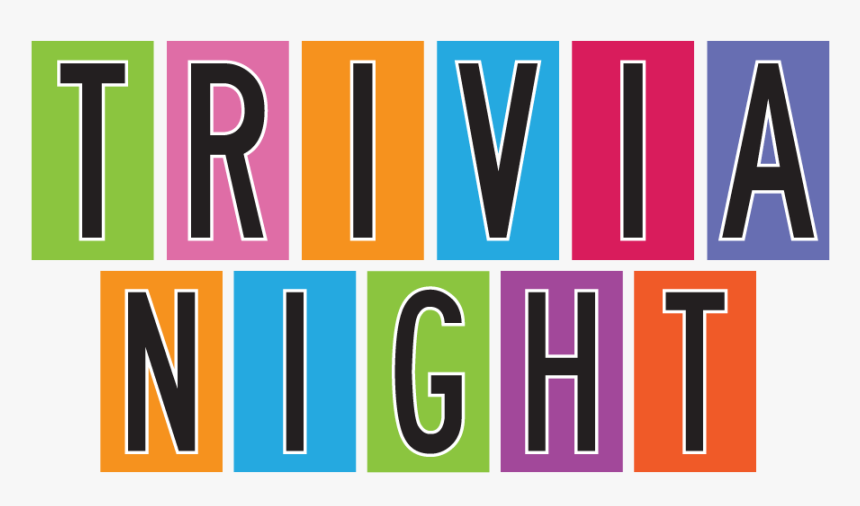
\includegraphics[max width=0.9\textwidth,
    max height=0.4\textheight]{Images/triviatitleframelogo.png}
\end{center}
\end{frame}

\begingroup{}
\begin{frame}[t]{}
Out of the 660 questions that we have posed so far, only three answers have been
 challenged. Nonetheless, we want to make sure that everyone who has a challenge has an
 opportunity to be heard, so we have retained a \mbox{Challenge Coordinator}.

\pause{}
\begin{center}
\begin{figure}[h]
\caption*{OUR CHALLENGE COORDINATOR}
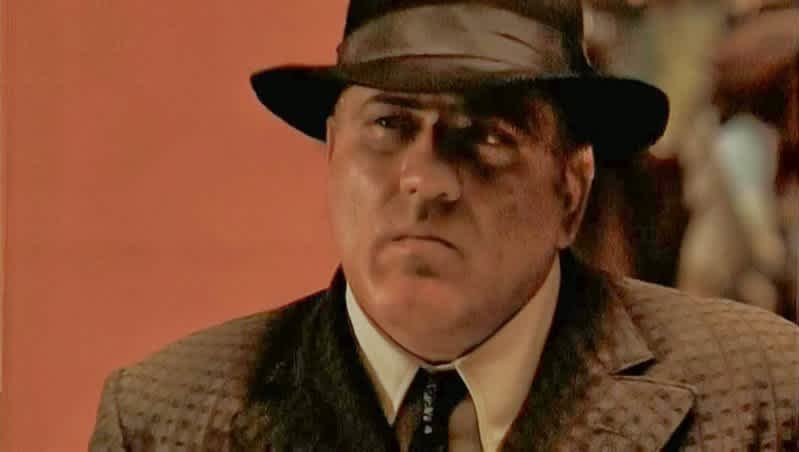
\includegraphics[max width=0.9\textwidth,
     max height=0.35\textheight]{Images/challengecoordinator.jpg}
\end{figure}
\end{center}
Please feel free to contact the Coordinator with any challenges.
For fastest resolution of your challenge, be sure to provide him with your home address.
\end{frame}
\endgroup{}

\begingroup{}
\begin{frame}[t]{Categories}
This week, you'll be answering questions in the following categories:
\begin{enumerate}
\item Album by Album Art
\item France
\item Airport Codes
\item Big Dates in History
\item Gangsters in Fact and Fiction
\item Holidays and Observances
\item All the Cool Kids are Texting about South Dakota
\item Pastries
\item Explorers
\item Products and Companies By Their Slogans
\end{enumerate}
\end{frame}
\endgroup{}

\begingroup{}
\begin{frame}
\vfill{}
\begin{beamercolorbox}[sep=8pt,center,shadow=true,rounded=true]{title}
\usebeamerfont{title}Good luck everyone! And have fun!
\end{beamercolorbox}
\vfill{}
\end{frame}
\endgroup{}
\def\thisSectionName{Album by Album Art}
\section{Round 1}
\subsection*{Q1}
\begin{frame}[t]{Round 1 --- Album by Album Art --- \mbox{Question 1}}
% \vspace{0.5em}
\begin{columns}[T,totalwidth=\linewidth]
\begin{column}{0.32\linewidth}
\begin{block}{Question}
Name the album.
\end{block}
\end{column}
\begin{column}{0.65\linewidth}
\begin{center}
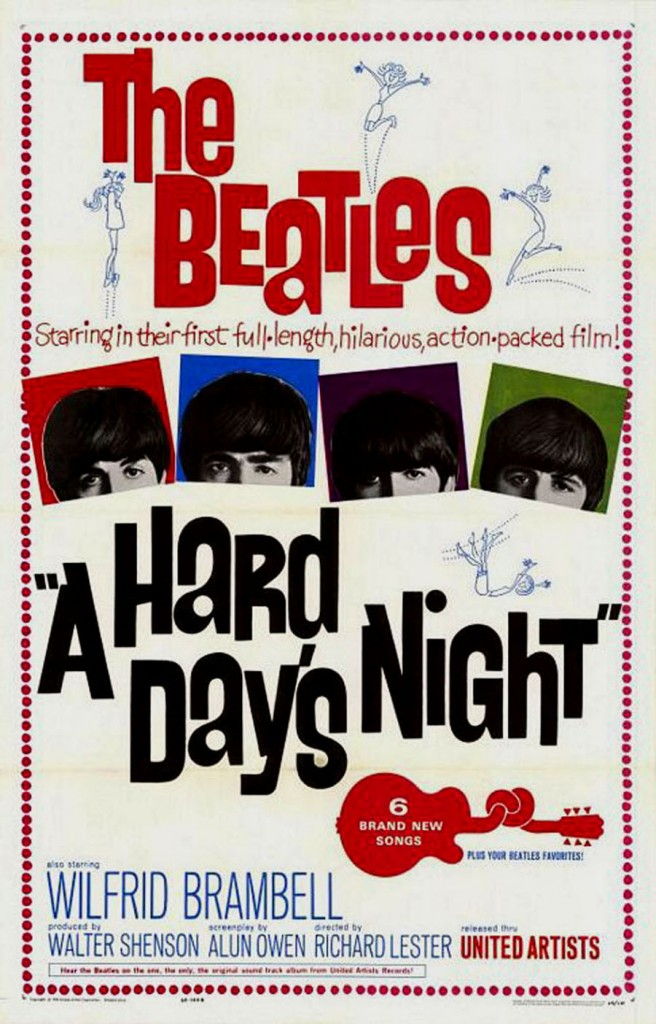
\includegraphics[max width=0.95\textwidth,max height=0.7\textheight]{{Images/harddaysnight}.jpeg}
\end{center}
\end{column}
\end{columns}
\end{frame}
\subsection*{Q2}
\begin{frame}[t]{Round 1 --- Album by Album Art --- \mbox{Question 2}}
% \vspace{0.5em}
\begin{columns}[T,totalwidth=\linewidth]
\begin{column}{0.32\linewidth}
\begin{block}{Question}
Name the album.
\end{block}
\end{column}
\begin{column}{0.65\linewidth}
\begin{center}
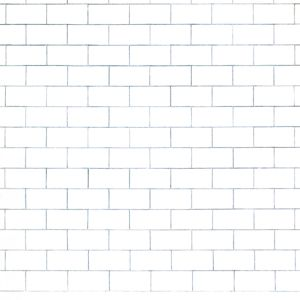
\includegraphics[max width=0.95\textwidth,max height=0.7\textheight]{{Images/thewall}.jpg}
\end{center}
\end{column}
\end{columns}
\end{frame}
\subsection*{Q3}
\begin{frame}[t]{Round 1 --- Album by Album Art --- \mbox{Question 3}}
% \vspace{0.5em}
\begin{columns}[T,totalwidth=\linewidth]
\begin{column}{0.32\linewidth}
\begin{block}{Question}
Name the album.
\end{block}
\end{column}
\begin{column}{0.65\linewidth}
\begin{center}
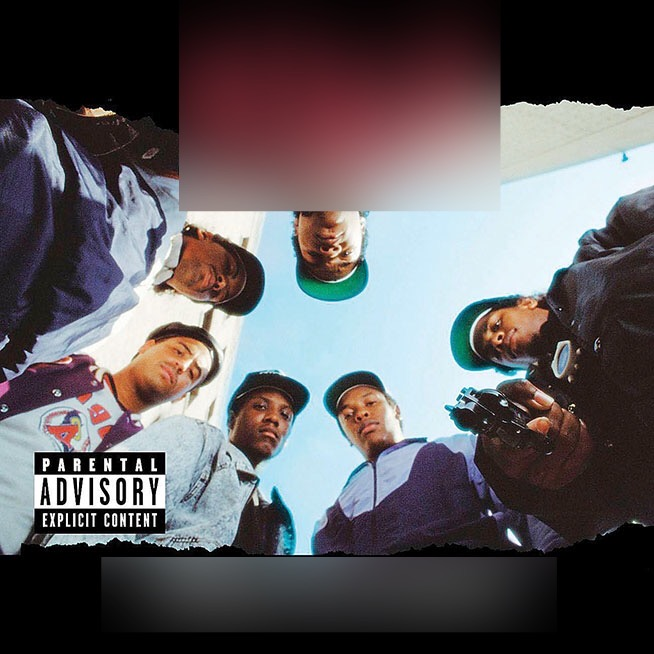
\includegraphics[max width=0.95\textwidth,max height=0.7\textheight]{{Images/straightouttacompton}.jpeg}
\end{center}
\end{column}
\end{columns}
\end{frame}
\subsection*{Q4}
\begin{frame}[t]{Round 1 --- Album by Album Art --- \mbox{Question 4}}
% \vspace{0.5em}
\begin{columns}[T,totalwidth=\linewidth]
\begin{column}{0.32\linewidth}
\begin{block}{Question}
Name the album.
\end{block}
\end{column}
\begin{column}{0.65\linewidth}
\begin{center}
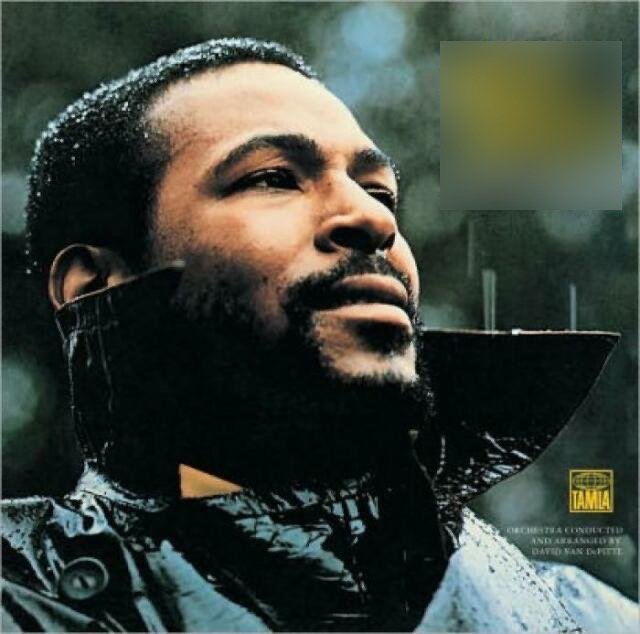
\includegraphics[max width=0.95\textwidth,max height=0.7\textheight]{{Images/whatsgoingon}.jpeg}
\end{center}
\end{column}
\end{columns}
\end{frame}
\subsection*{Q5}
\begin{frame}[t]{Round 1 --- Album by Album Art --- \mbox{Question 5}}
% \vspace{0.5em}
\begin{columns}[T,totalwidth=\linewidth]
\begin{column}{0.32\linewidth}
\begin{block}{Question}
Name the album.
\end{block}
\end{column}
\begin{column}{0.65\linewidth}
\begin{center}
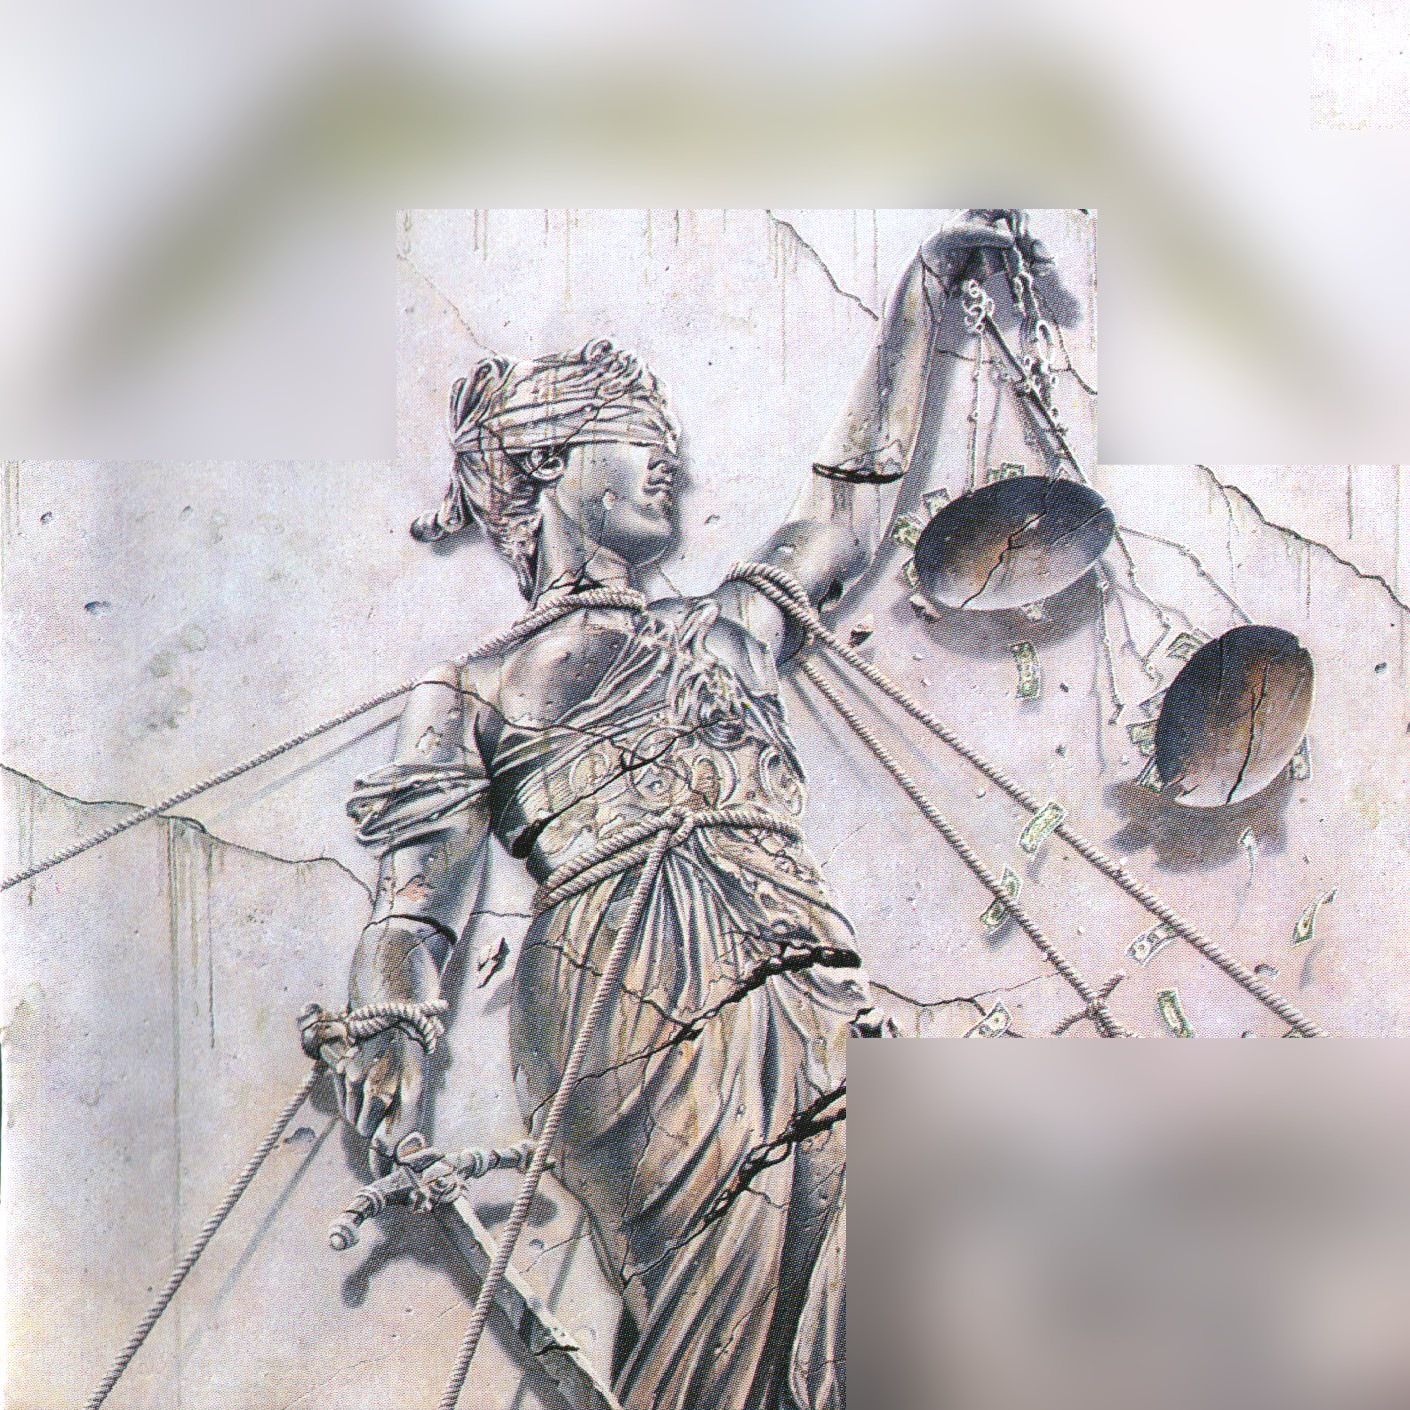
\includegraphics[max width=0.95\textwidth,max height=0.7\textheight]{{Images/andjusticeforall}.jpeg}
\end{center}
\end{column}
\end{columns}
\end{frame}
\subsection*{Q6}
\begin{frame}[t]{Round 1 --- Album by Album Art --- \mbox{Question 6}}
% \vspace{0.5em}
\begin{columns}[T,totalwidth=\linewidth]
\begin{column}{0.32\linewidth}
\begin{block}{Question}
Name the album.
\end{block}
\end{column}
\begin{column}{0.65\linewidth}
\begin{center}
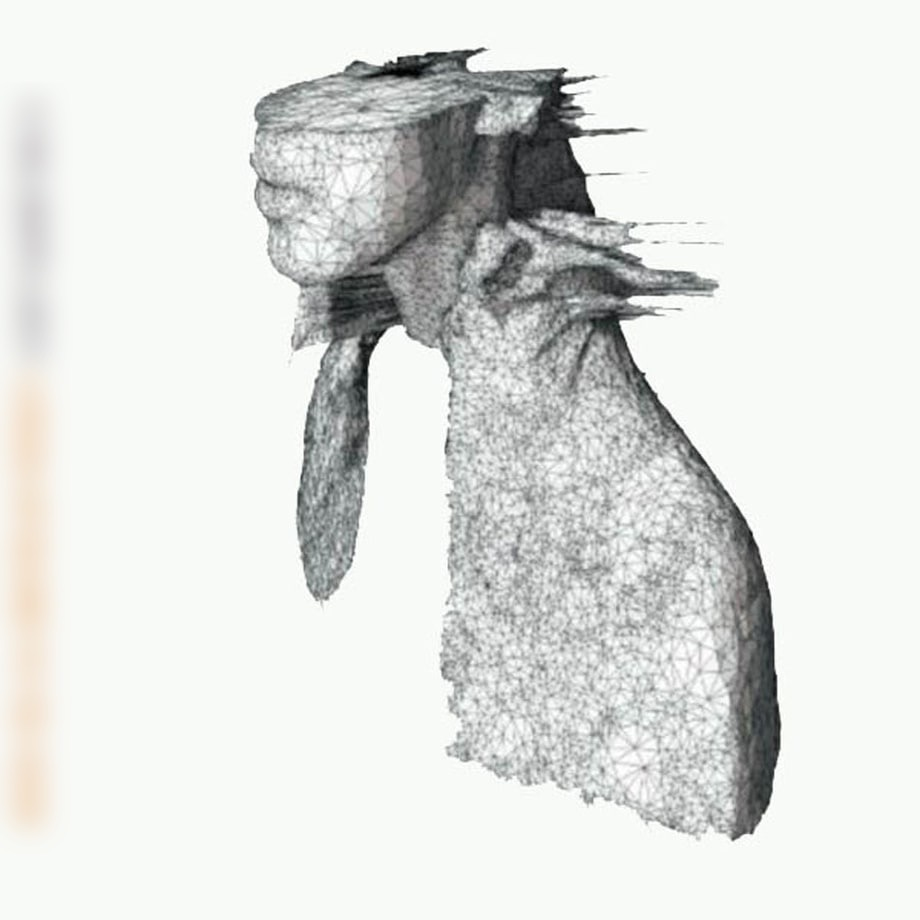
\includegraphics[max width=0.95\textwidth,max height=0.7\textheight]{{Images/rushofblood}.jpeg}
\end{center}
\end{column}
\end{columns}
\end{frame}
\subsection*{Q7}
\begin{frame}[t]{Round 1 --- Album by Album Art --- \mbox{Question 7}}
% \vspace{0.5em}
\begin{columns}[T,totalwidth=\linewidth]
\begin{column}{0.32\linewidth}
\begin{block}{Question}
Name the album.
\end{block}
\end{column}
\begin{column}{0.65\linewidth}
\begin{center}
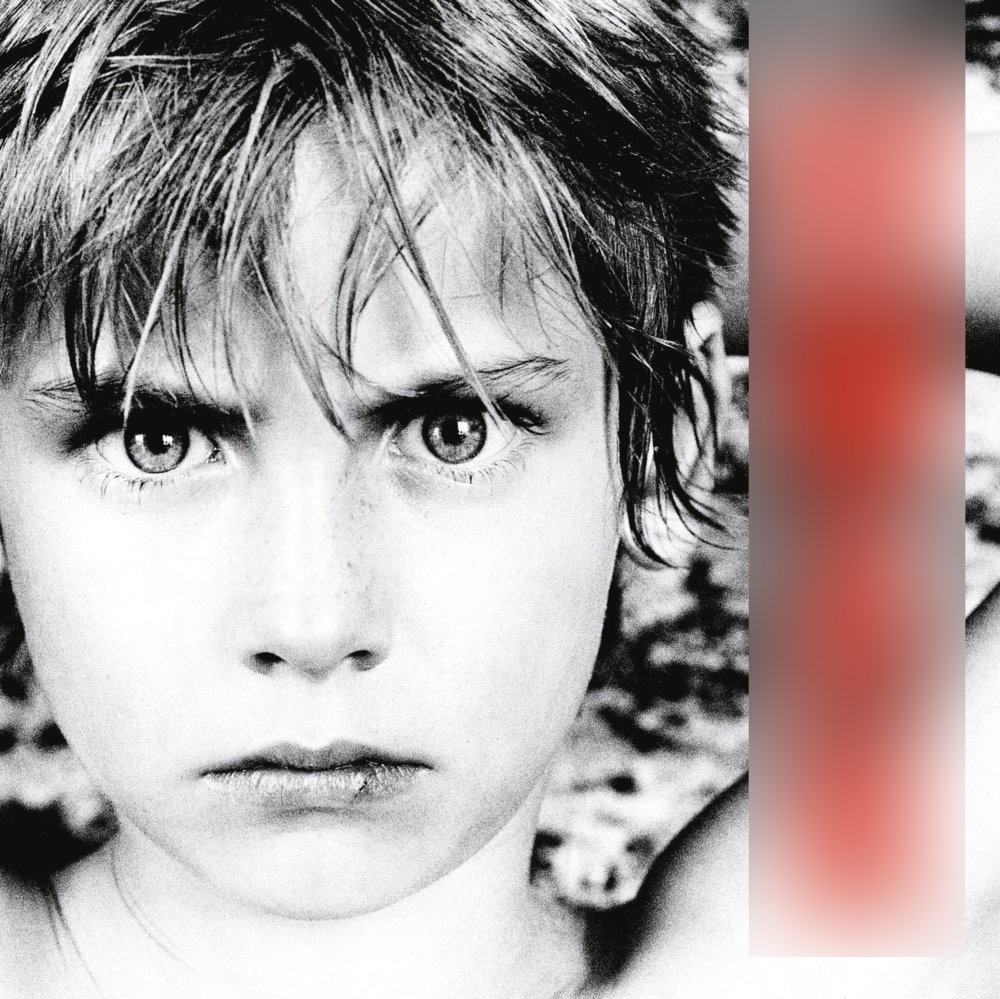
\includegraphics[max width=0.95\textwidth,max height=0.7\textheight]{{Images/u2war}.jpeg}
\end{center}
\end{column}
\end{columns}
\end{frame}
\subsection*{Q8}
\begin{frame}[t]{Round 1 --- Album by Album Art --- \mbox{Question 8}}
% \vspace{0.5em}
\begin{columns}[T,totalwidth=\linewidth]
\begin{column}{0.32\linewidth}
\begin{block}{Question}
Name the album.
\end{block}
\end{column}
\begin{column}{0.65\linewidth}
\begin{center}
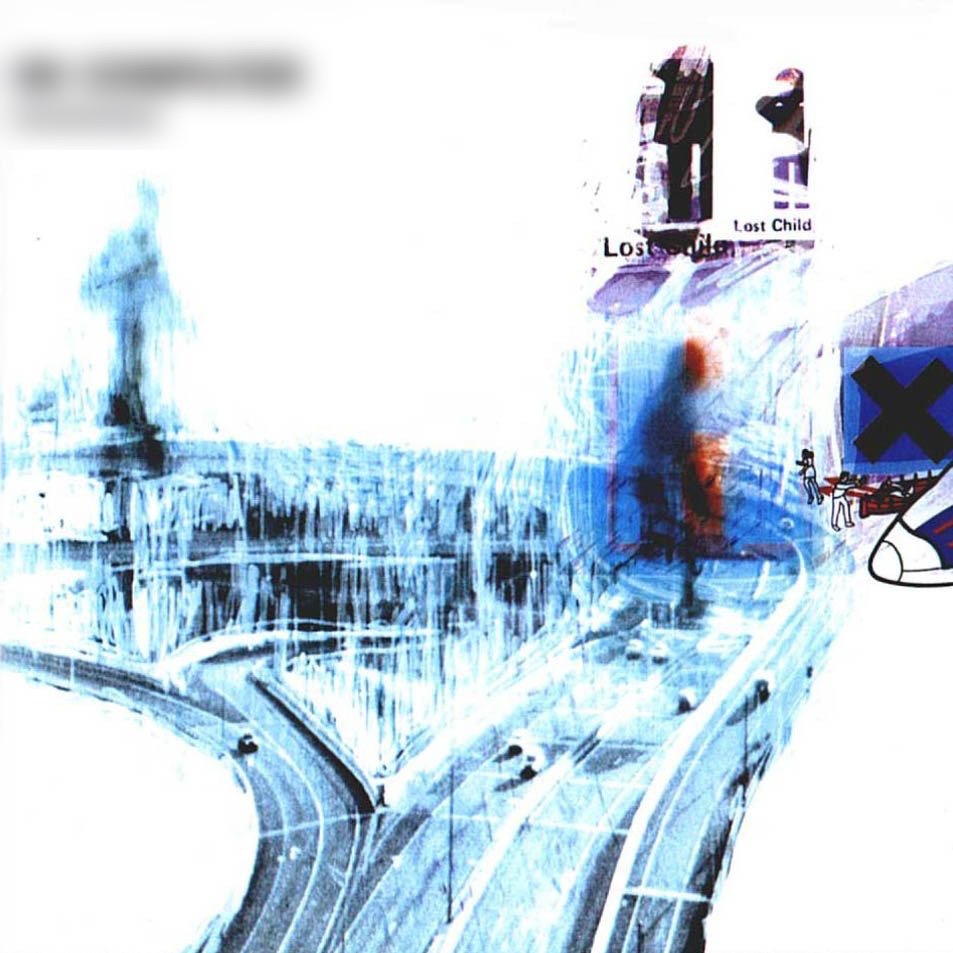
\includegraphics[max width=0.95\textwidth,max height=0.7\textheight]{{Images/okcomputer}.jpeg}
\end{center}
\end{column}
\end{columns}
\end{frame}
\subsection*{Q9}
\begin{frame}[t]{Round 1 --- Album by Album Art --- \mbox{Question 9}}
% \vspace{0.5em}
\begin{columns}[T,totalwidth=\linewidth]
\begin{column}{0.32\linewidth}
\begin{block}{Question}
Name the album.
\end{block}
\end{column}
\begin{column}{0.65\linewidth}
\begin{center}
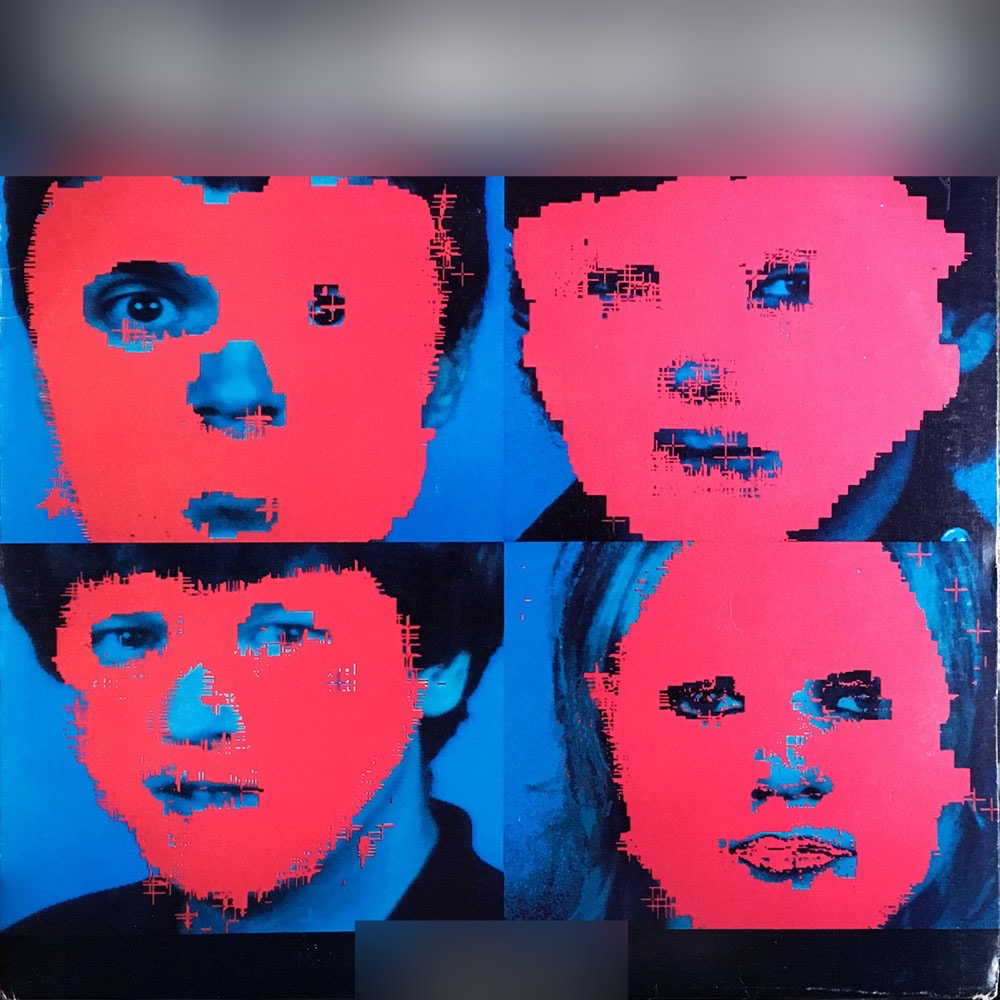
\includegraphics[max width=0.95\textwidth,max height=0.7\textheight]{{Images/remaininlight}.jpeg}
\end{center}
\end{column}
\end{columns}
\end{frame}
\subsection*{Q10}
\begin{frame}[t]{Round 1 --- Album by Album Art --- \mbox{Question 10}}
% \vspace{0.5em}
\begin{columns}[T,totalwidth=\linewidth]
\begin{column}{0.32\linewidth}
\begin{block}{Question}
Name the album.
\end{block}
\end{column}
\begin{column}{0.65\linewidth}
\begin{center}
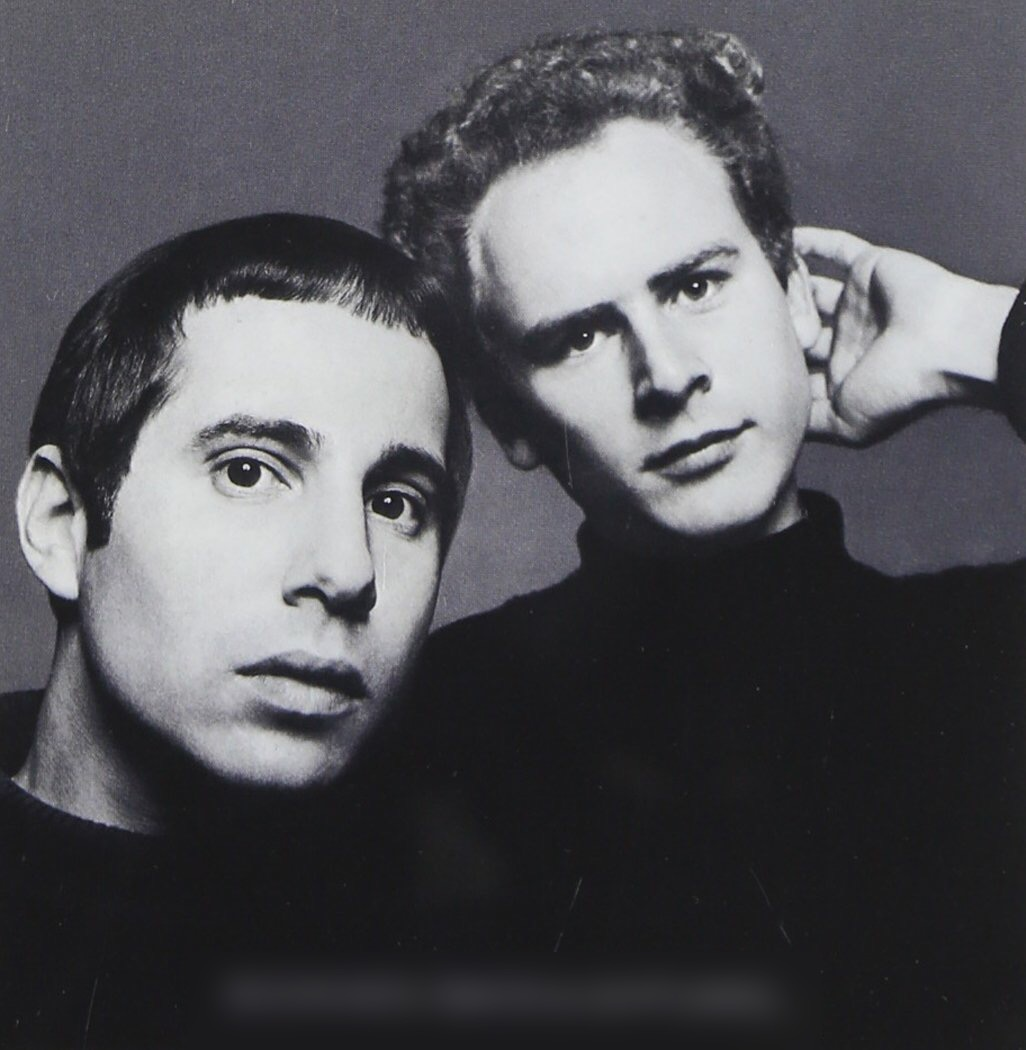
\includegraphics[max width=0.95\textwidth,max height=0.7\textheight]{{Images/bookends}.jpeg}
\end{center}
\end{column}
\end{columns}
\end{frame}
\subsection{Answers}
\begin{frame}[t]{Round 1 --- Album by Album Art --- \mbox{Answer 1}}
% \vspace{0.5em}
\begin{columns}[T,totalwidth=\linewidth]
\begin{column}{0.32\linewidth}
\begin{block}{Question}
Name the album.
\end{block}
\end{column}
\begin{column}{0.65\linewidth}
\begin{center}
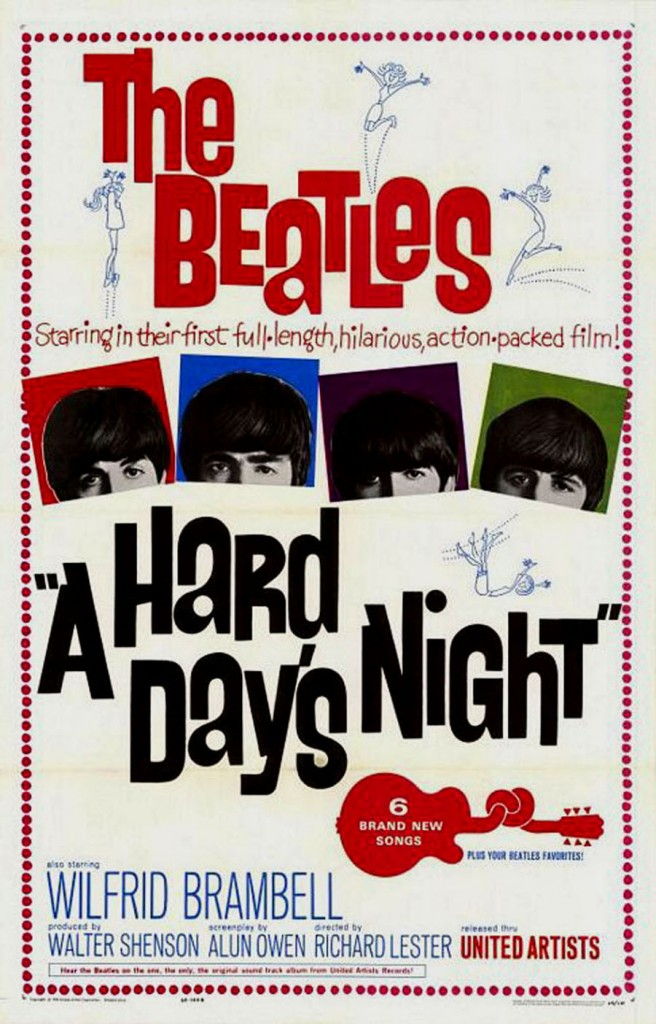
\includegraphics[max width=0.95\textwidth,max height=0.35\textheight]{{Images/harddaysnight}.jpeg}
\end{center}
\end{column}
\end{columns}

\visible<2->{
    \begin{columns}[T,totalwidth=\linewidth]
    \begin{column}{0.32\linewidth}
    \begin{block}{Answer}
    \emph{A Hard Day's Night} (The Beatles)
    \end{block}
    \end{column}
    \begin{column}{0.65\linewidth}
    \begin{center}
    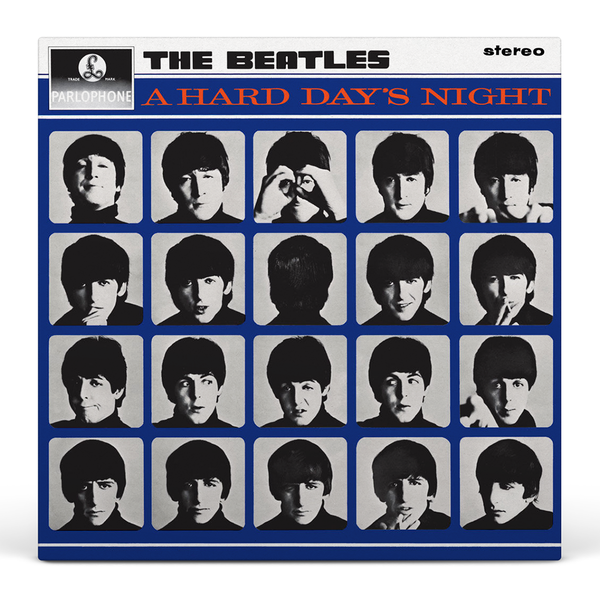
\includegraphics[max width=0.95\textwidth,
        max height=0.38\textheight]{{Images/harddaysnightanswer}.png}
    \end{center}
    \end{column}
    \end{columns}
}
\end{frame}
\begin{frame}[t]{Round 1 --- Album by Album Art --- \mbox{Answer 2}}
% \vspace{0.5em}
\begin{columns}[T,totalwidth=\linewidth]
\begin{column}{0.32\linewidth}
\begin{block}{Question}
Name the album.
\end{block}
\end{column}
\begin{column}{0.65\linewidth}
\begin{center}
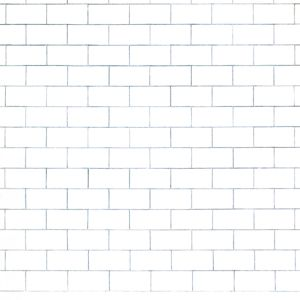
\includegraphics[max width=0.95\textwidth,max height=0.35\textheight]{{Images/thewall}.jpg}
\end{center}
\end{column}
\end{columns}

\visible<2->{
    \begin{columns}[T,totalwidth=\linewidth]
    \begin{column}{0.32\linewidth}
    \begin{block}{Answer}
     \emph{The Wall} (Pink Floyd)
    \end{block}
    \end{column}
    \begin{column}{0.65\linewidth}
    \begin{center}
    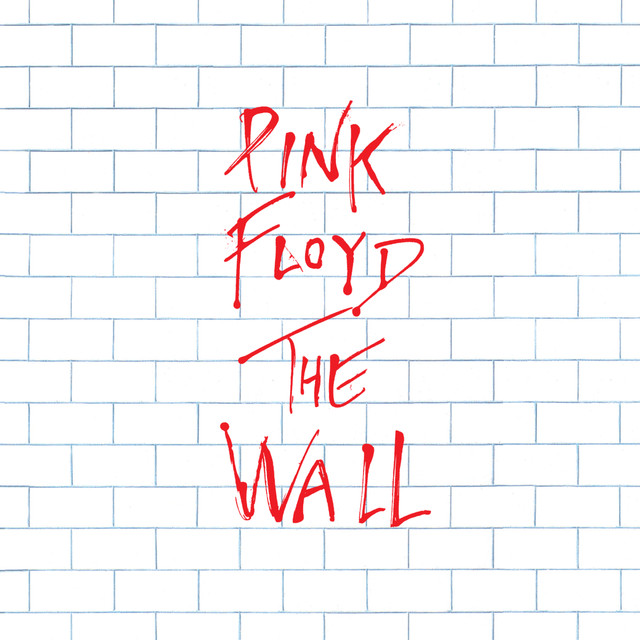
\includegraphics[max width=0.95\textwidth,
        max height=0.38\textheight]{{Images/wallanswer}.jpeg}
    \end{center}
    \end{column}
    \end{columns}
}
\end{frame}
\begin{frame}[t]{Round 1 --- Album by Album Art --- \mbox{Answer 3}}
% \vspace{0.5em}
\begin{columns}[T,totalwidth=\linewidth]
\begin{column}{0.32\linewidth}
\begin{block}{Question}
Name the album.
\end{block}
\end{column}
\begin{column}{0.65\linewidth}
\begin{center}
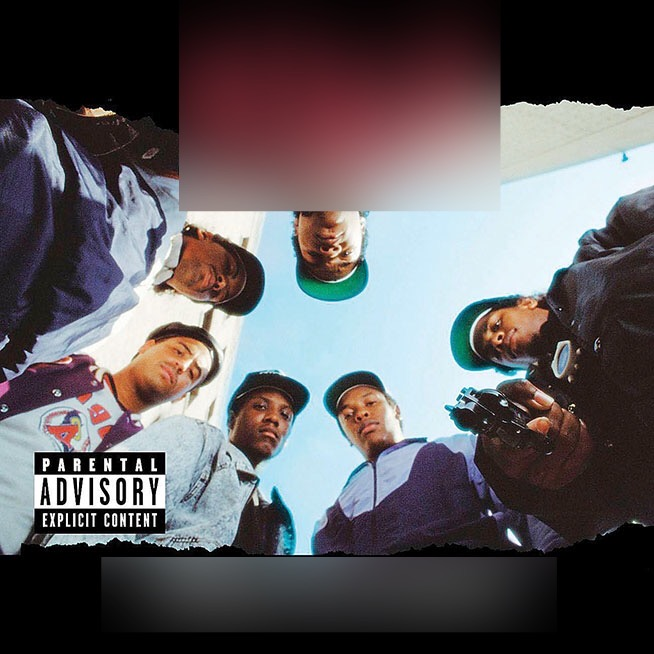
\includegraphics[max width=0.95\textwidth,max height=0.35\textheight]{{Images/straightouttacompton}.jpeg}
\end{center}
\end{column}
\end{columns}

\visible<2->{
    \begin{columns}[T,totalwidth=\linewidth]
    \begin{column}{0.32\linewidth}
    \begin{block}{Answer}
    \emph{Straight Outta Compton} (N.\@W.\@A)
    \end{block}
    \end{column}
    \begin{column}{0.65\linewidth}
    \begin{center}
    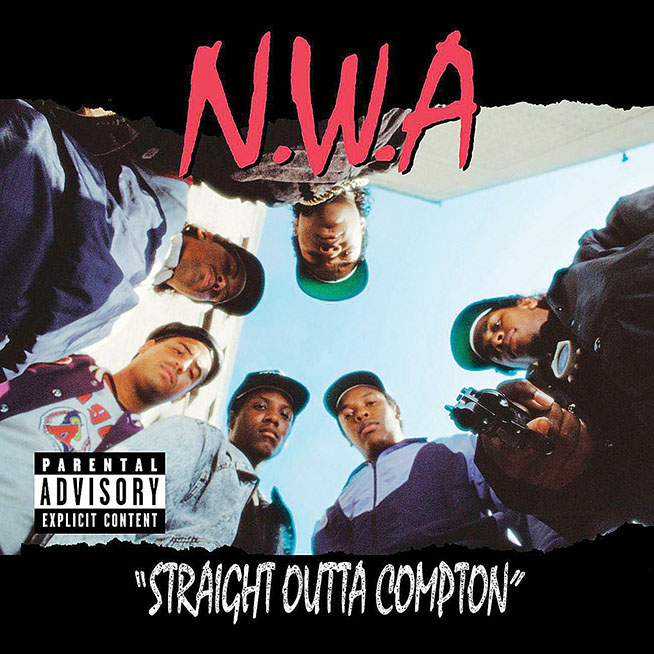
\includegraphics[max width=0.95\textwidth,
        max height=0.38\textheight]{{Images/comptonanswer}.jpeg}
    \end{center}
    \end{column}
    \end{columns}
}
\end{frame}
\begin{frame}[t]{Round 1 --- Album by Album Art --- \mbox{Answer 4}}
% \vspace{0.5em}
\begin{columns}[T,totalwidth=\linewidth]
\begin{column}{0.32\linewidth}
\begin{block}{Question}
Name the album.
\end{block}
\end{column}
\begin{column}{0.65\linewidth}
\begin{center}
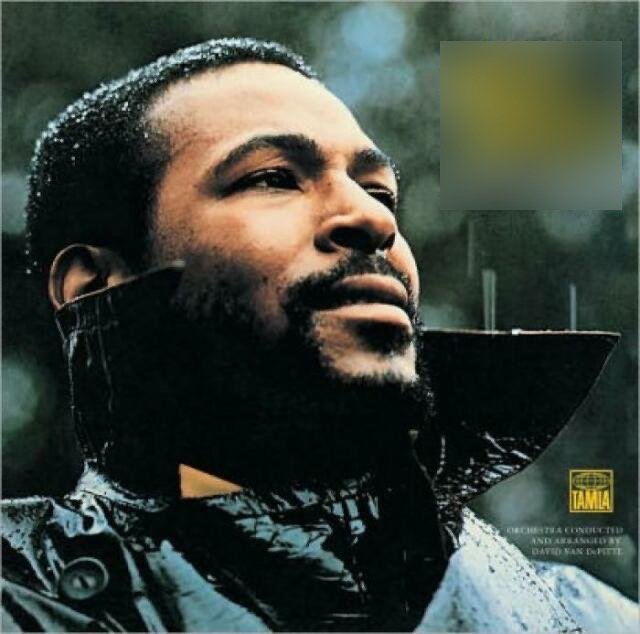
\includegraphics[max width=0.95\textwidth,max height=0.35\textheight]{{Images/whatsgoingon}.jpeg}
\end{center}
\end{column}
\end{columns}

\visible<2->{
    \begin{columns}[T,totalwidth=\linewidth]
    \begin{column}{0.32\linewidth}
    \begin{block}{Answer}
    \emph{What's Going On} (Marvin Gaye)
    \end{block}
    \end{column}
    \begin{column}{0.65\linewidth}
    \begin{center}
    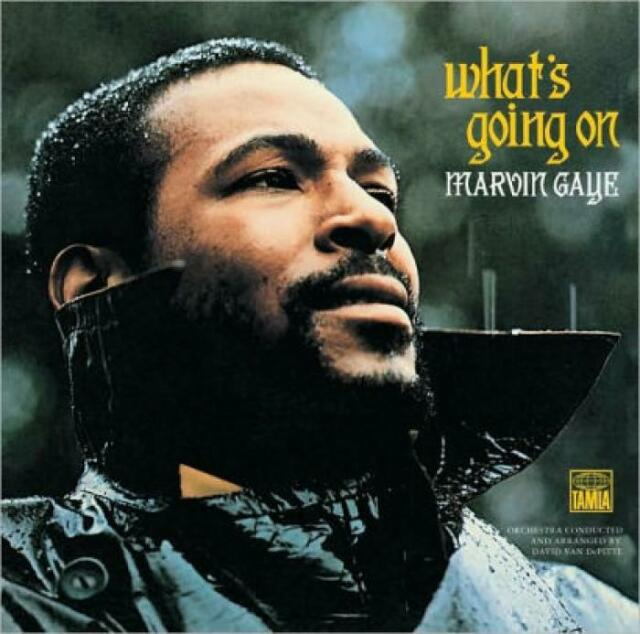
\includegraphics[max width=0.95\textwidth,
        max height=0.38\textheight]{{Images/gayeanswer}.jpeg}
    \end{center}
    \end{column}
    \end{columns}
}
\end{frame}
\begin{frame}[t]{Round 1 --- Album by Album Art --- \mbox{Answer 5}}
% \vspace{0.5em}
\begin{columns}[T,totalwidth=\linewidth]
\begin{column}{0.32\linewidth}
\begin{block}{Question}
Name the album.
\end{block}
\end{column}
\begin{column}{0.65\linewidth}
\begin{center}
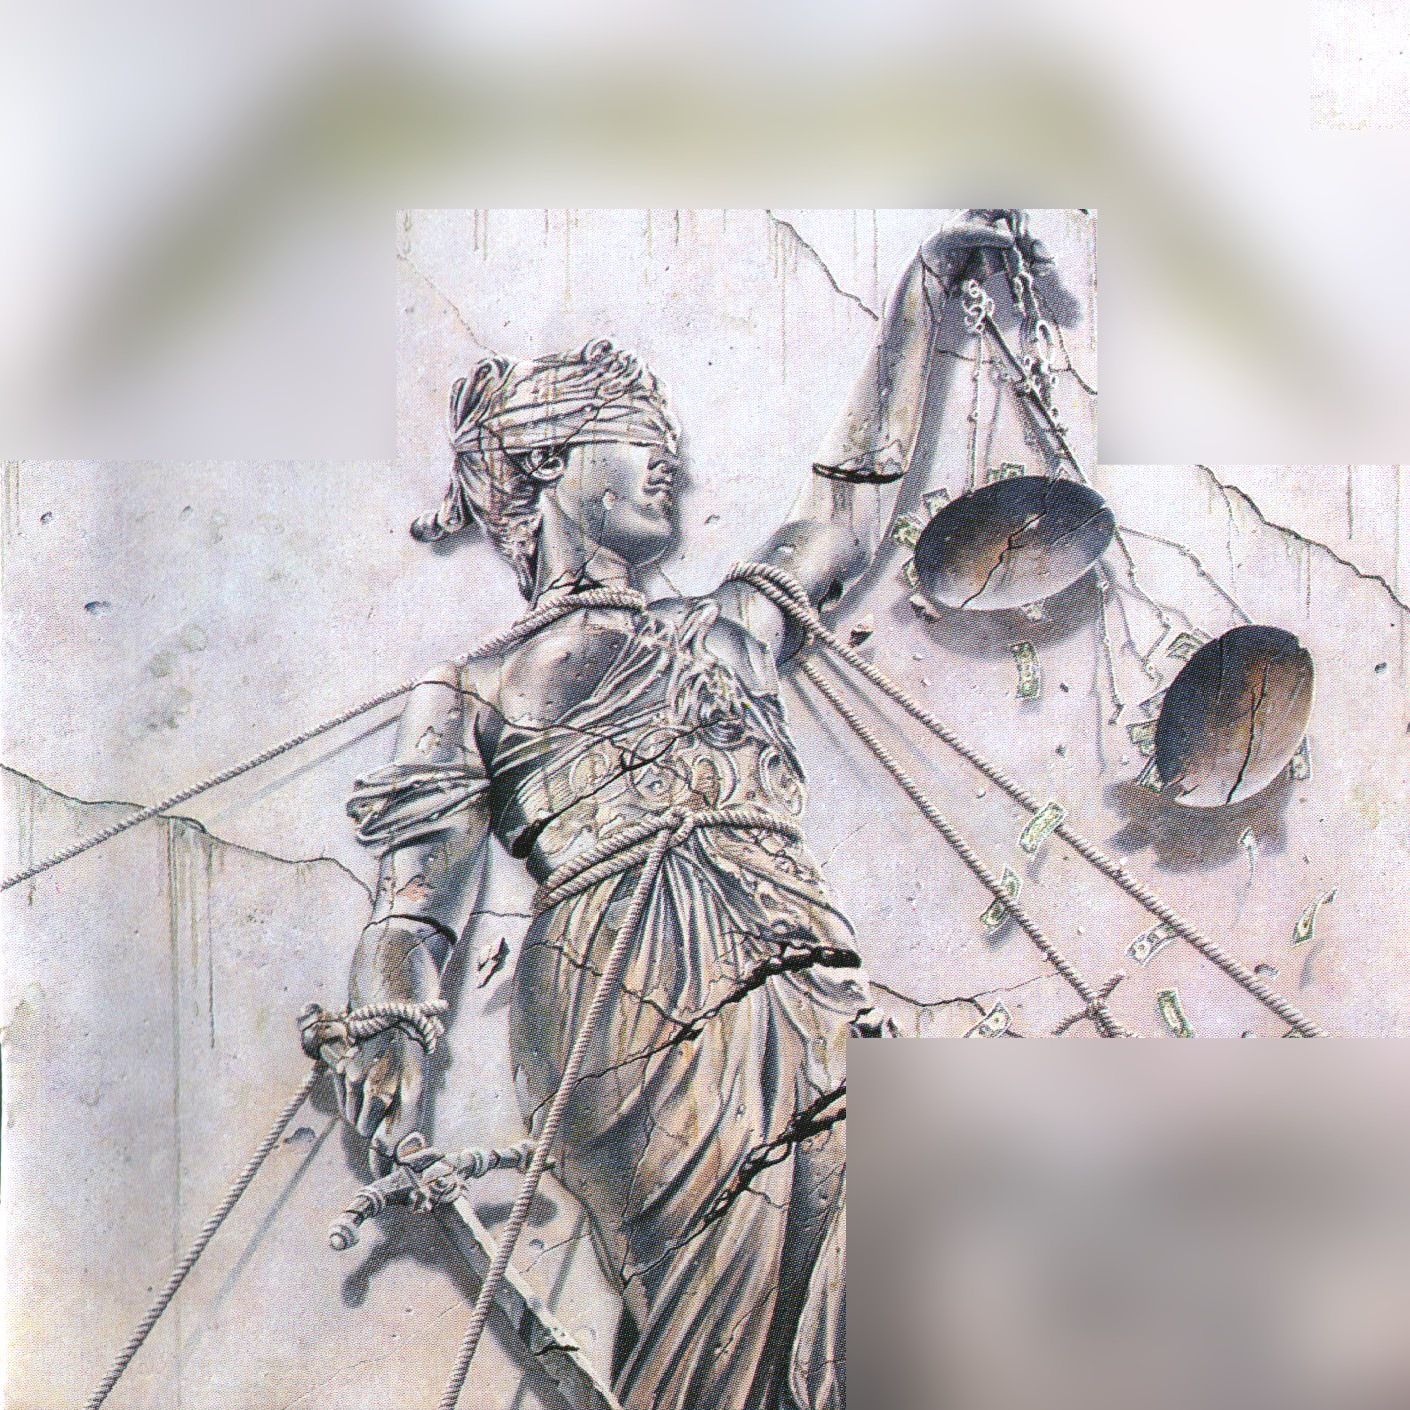
\includegraphics[max width=0.95\textwidth,max height=0.35\textheight]{{Images/andjusticeforall}.jpeg}
\end{center}
\end{column}
\end{columns}

\visible<2->{
    \begin{columns}[T,totalwidth=\linewidth]
    \begin{column}{0.32\linewidth}
    \begin{block}{Answer}
    \emph{\ldots{}And Justice For All} (Metallica)
    \end{block}
    \end{column}
    \begin{column}{0.65\linewidth}
    \begin{center}
    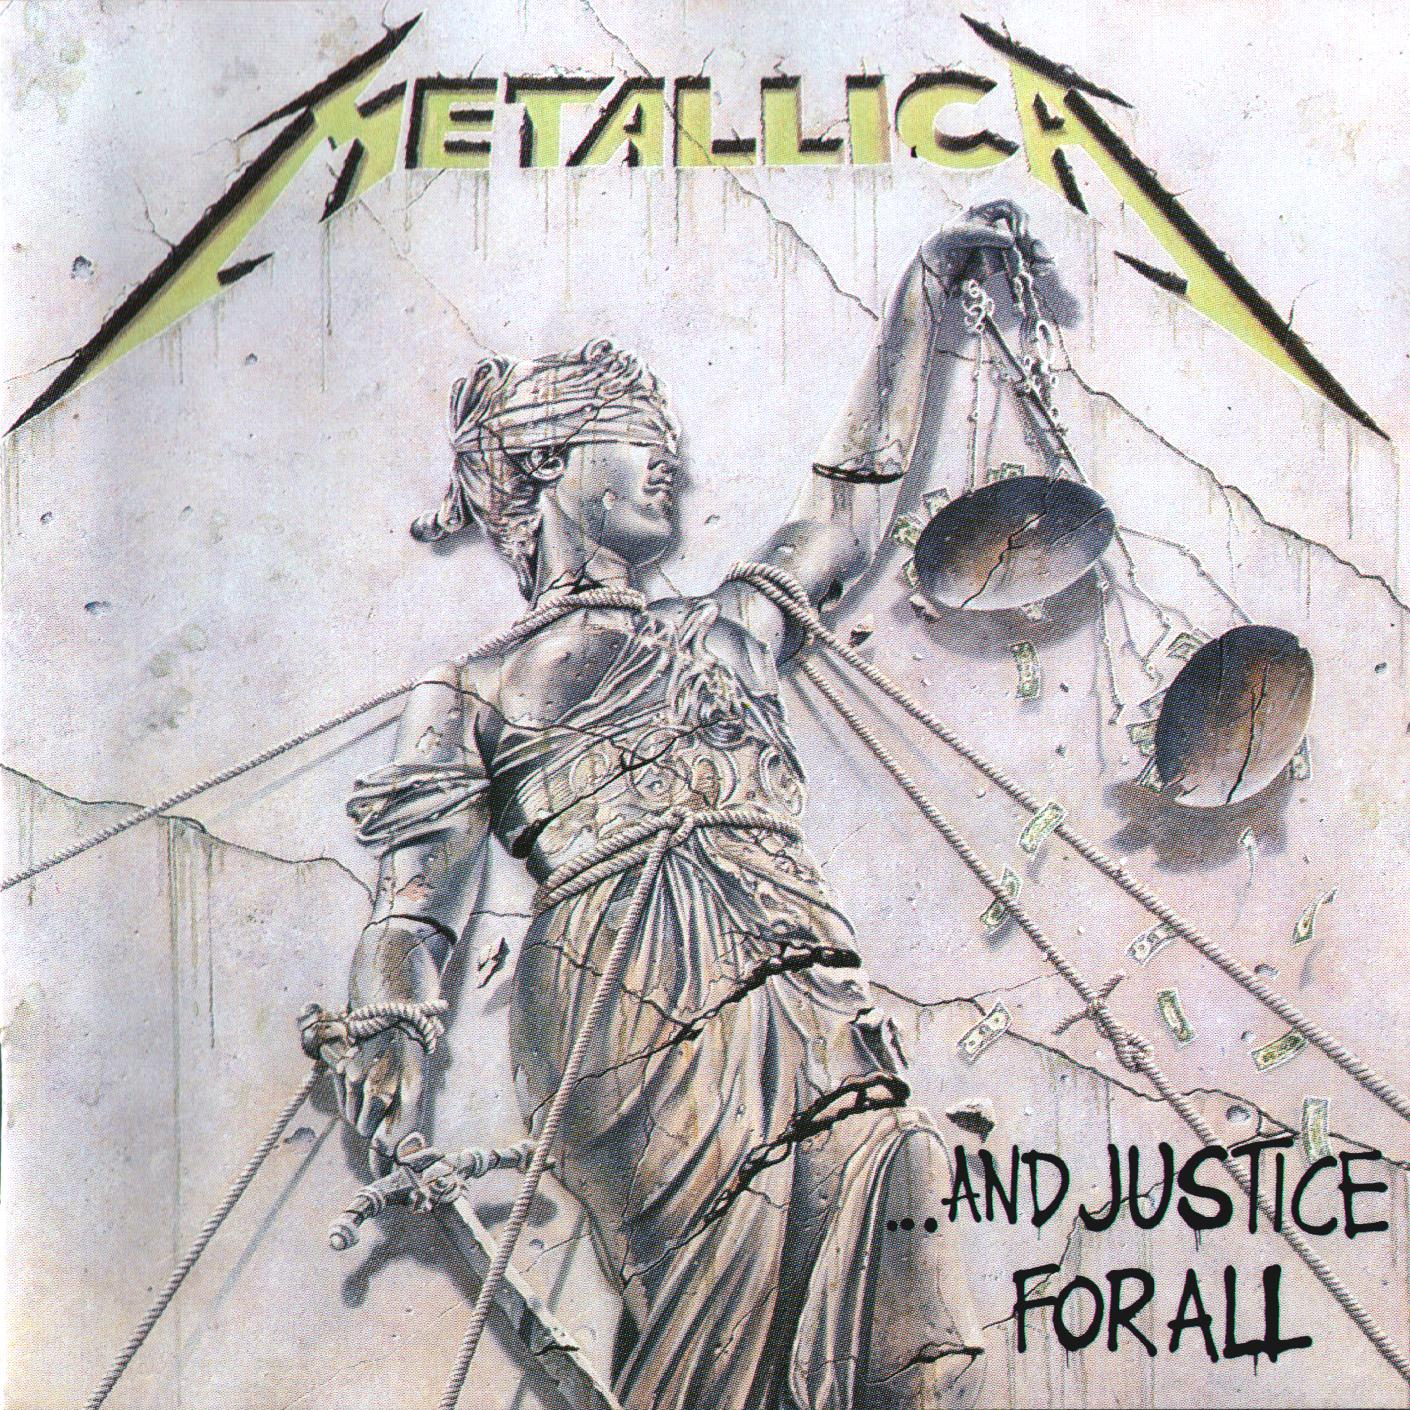
\includegraphics[max width=0.95\textwidth,
        max height=0.38\textheight]{{Images/justiceanswer}.jpeg}
    \end{center}
    \end{column}
    \end{columns}
}
\end{frame}
\begin{frame}[t]{Round 1 --- Album by Album Art --- \mbox{Answer 6}}
% \vspace{0.5em}
\begin{columns}[T,totalwidth=\linewidth]
\begin{column}{0.32\linewidth}
\begin{block}{Question}
Name the album.
\end{block}
\end{column}
\begin{column}{0.65\linewidth}
\begin{center}
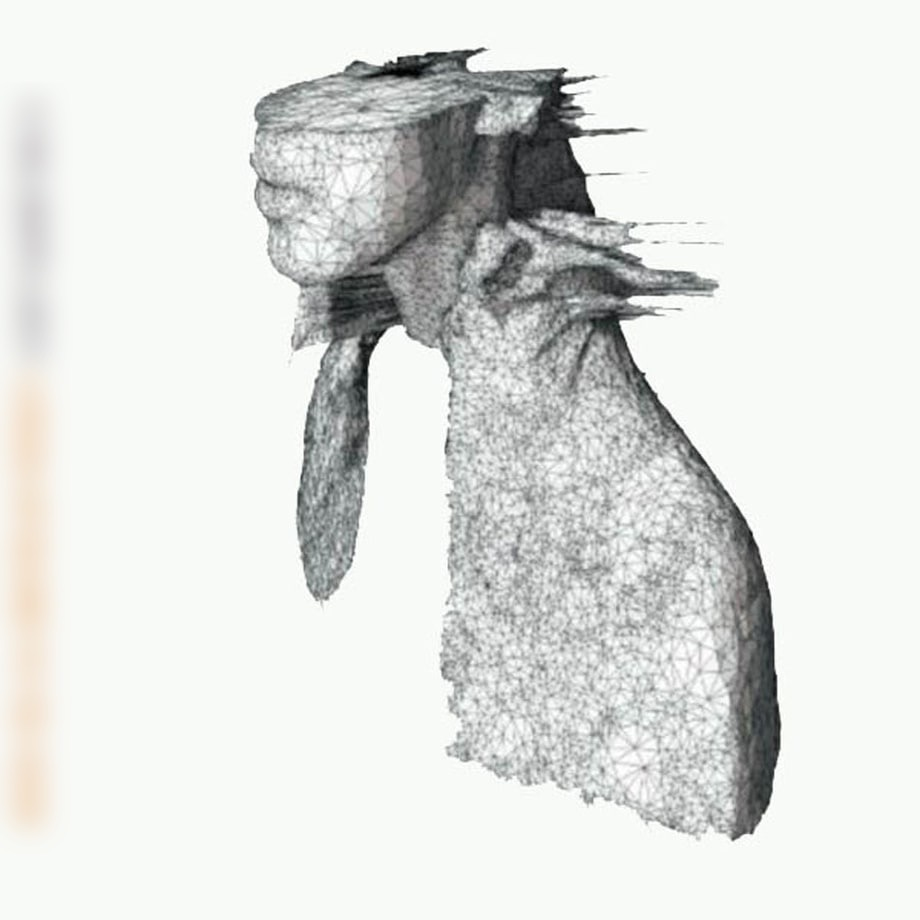
\includegraphics[max width=0.95\textwidth,max height=0.35\textheight]{{Images/rushofblood}.jpeg}
\end{center}
\end{column}
\end{columns}

\visible<2->{
    \begin{columns}[T,totalwidth=\linewidth]
    \begin{column}{0.32\linewidth}
    \begin{block}{Answer}
    \emph{A Rush of Blood to the Head} (Coldplay)
    \end{block}
    \end{column}
    \begin{column}{0.65\linewidth}
    \begin{center}
    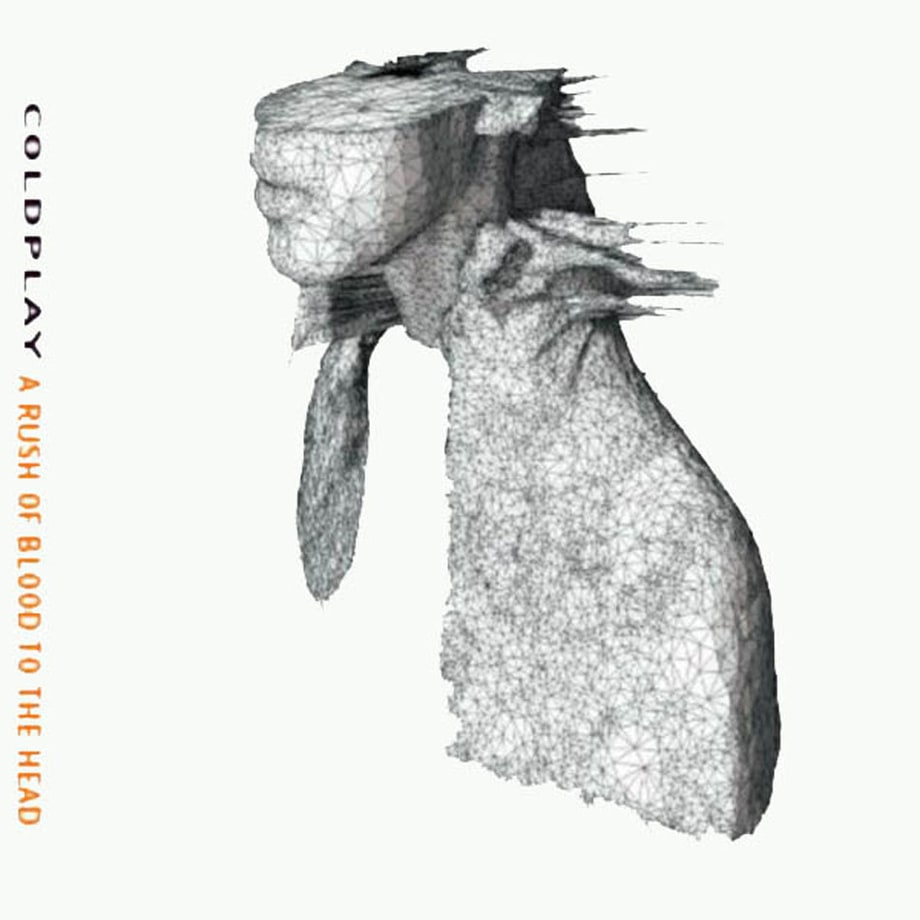
\includegraphics[max width=0.95\textwidth,
        max height=0.38\textheight]{{Images/rushanswer}.jpeg}
    \end{center}
    \end{column}
    \end{columns}
}
\end{frame}
\begin{frame}[t]{Round 1 --- Album by Album Art --- \mbox{Answer 7}}
% \vspace{0.5em}
\begin{columns}[T,totalwidth=\linewidth]
\begin{column}{0.32\linewidth}
\begin{block}{Question}
Name the album.
\end{block}
\end{column}
\begin{column}{0.65\linewidth}
\begin{center}
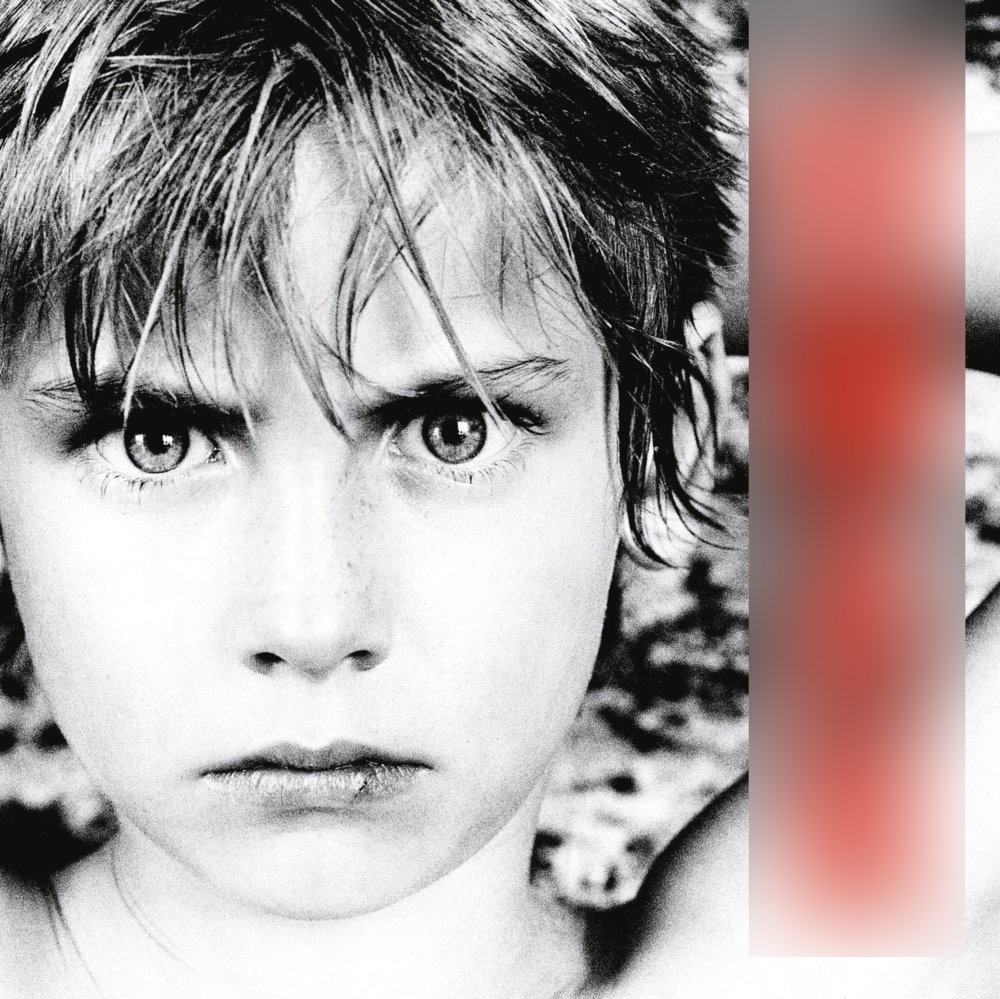
\includegraphics[max width=0.95\textwidth,max height=0.35\textheight]{{Images/u2war}.jpeg}
\end{center}
\end{column}
\end{columns}

\visible<2->{
    \begin{columns}[T,totalwidth=\linewidth]
    \begin{column}{0.32\linewidth}
    \begin{block}{Answer}
    \emph{War} (U2)
    \end{block}
    \end{column}
    \begin{column}{0.65\linewidth}
    \begin{center}
    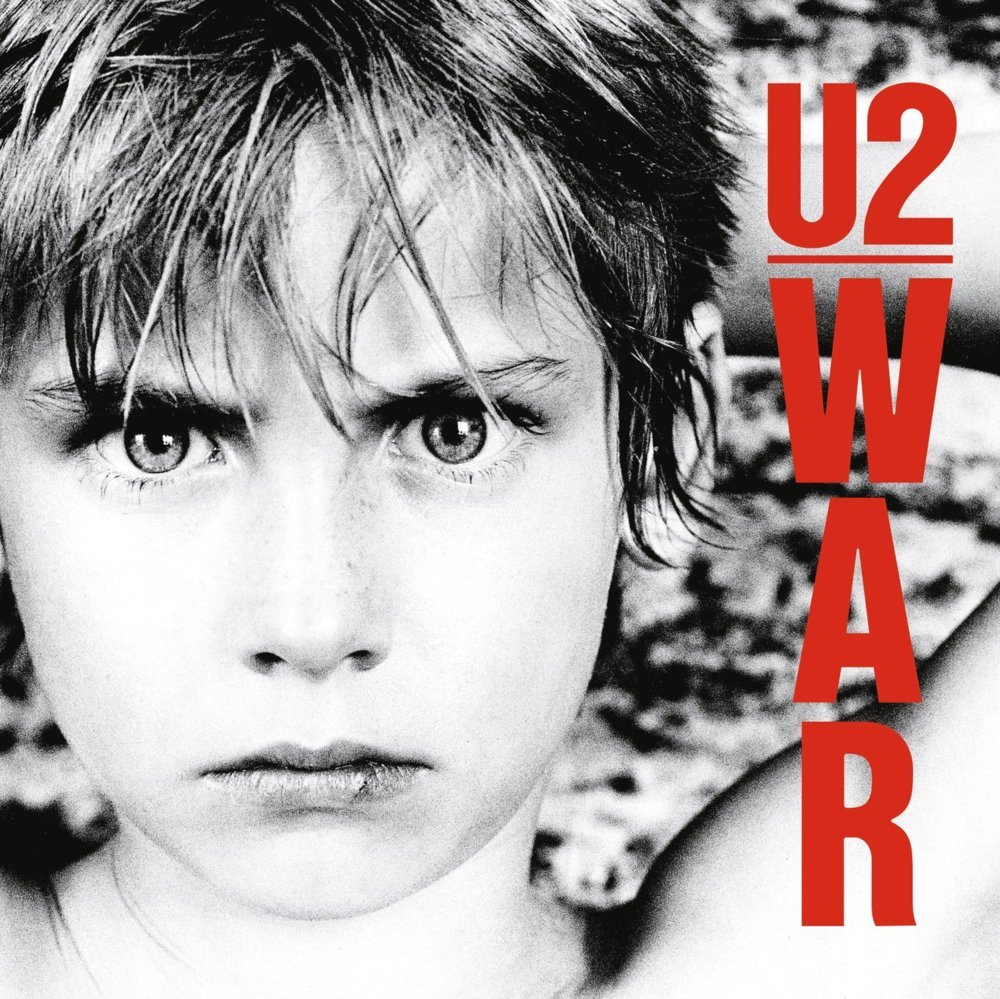
\includegraphics[max width=0.95\textwidth,
        max height=0.38\textheight]{{Images/waranswer}.jpeg}
    \end{center}
    \end{column}
    \end{columns}
}
\end{frame}
\begin{frame}[t]{Round 1 --- Album by Album Art --- \mbox{Answer 8}}
% \vspace{0.5em}
\begin{columns}[T,totalwidth=\linewidth]
\begin{column}{0.32\linewidth}
\begin{block}{Question}
Name the album.
\end{block}
\end{column}
\begin{column}{0.65\linewidth}
\begin{center}
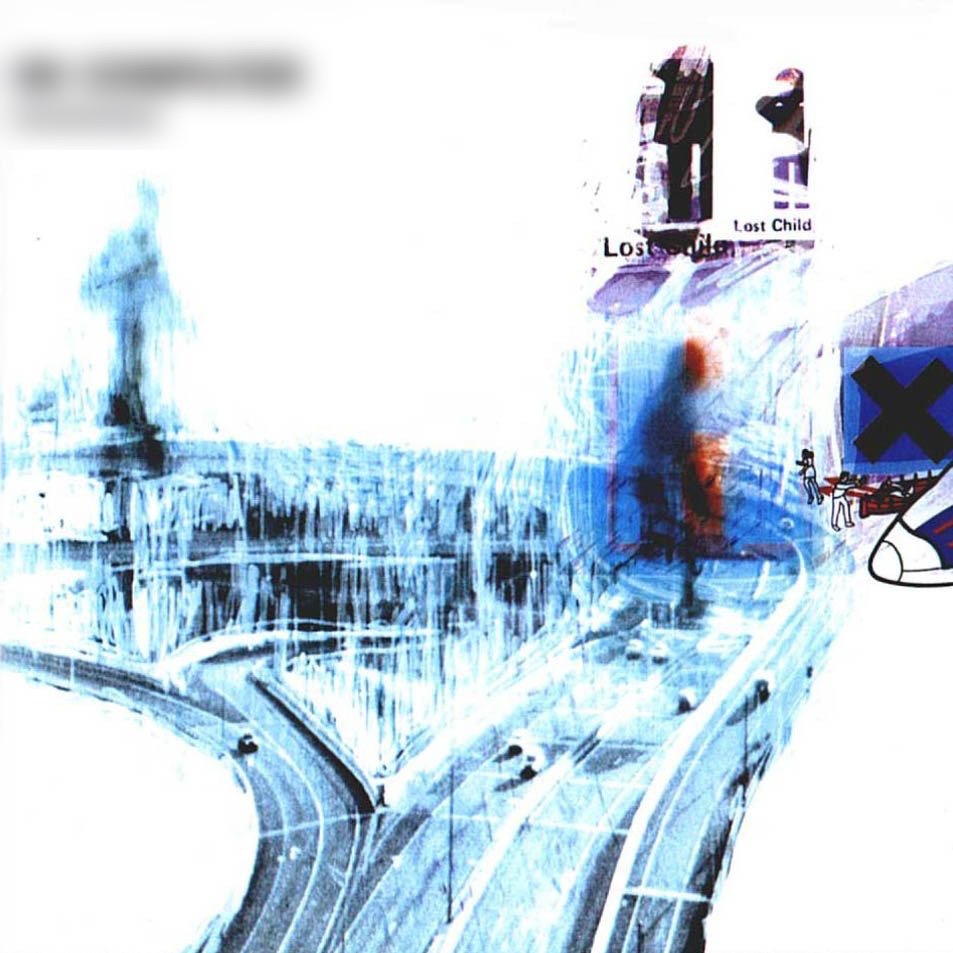
\includegraphics[max width=0.95\textwidth,max height=0.35\textheight]{{Images/okcomputer}.jpeg}
\end{center}
\end{column}
\end{columns}

\visible<2->{
    \begin{columns}[T,totalwidth=\linewidth]
    \begin{column}{0.32\linewidth}
    \begin{block}{Answer}
    \emph{OK Computer} (Radiohead)
    \end{block}
    \end{column}
    \begin{column}{0.65\linewidth}
    \begin{center}
    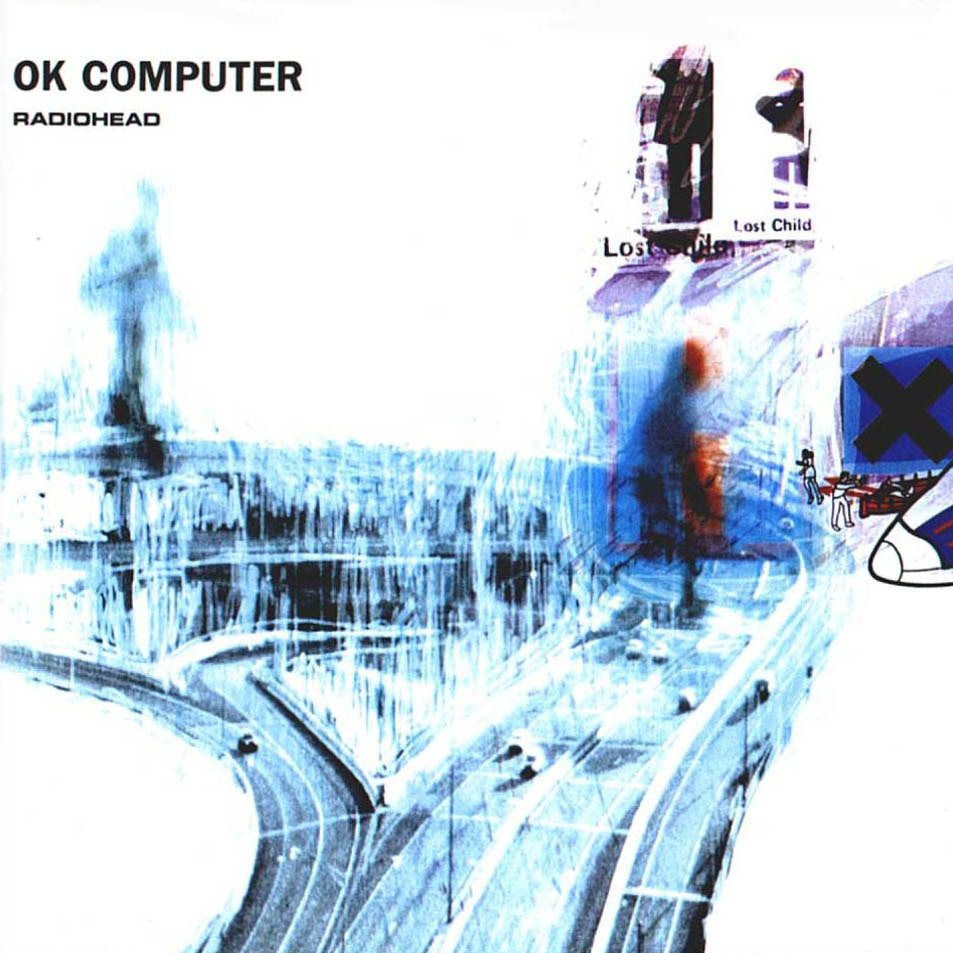
\includegraphics[max width=0.95\textwidth,
        max height=0.38\textheight]{{Images/okcompanswer}.jpeg}
    \end{center}
    \end{column}
    \end{columns}
}
\end{frame}
\begin{frame}[t]{Round 1 --- Album by Album Art --- \mbox{Answer 9}}
% \vspace{0.5em}
\begin{columns}[T,totalwidth=\linewidth]
\begin{column}{0.32\linewidth}
\begin{block}{Question}
Name the album.
\end{block}
\end{column}
\begin{column}{0.65\linewidth}
\begin{center}
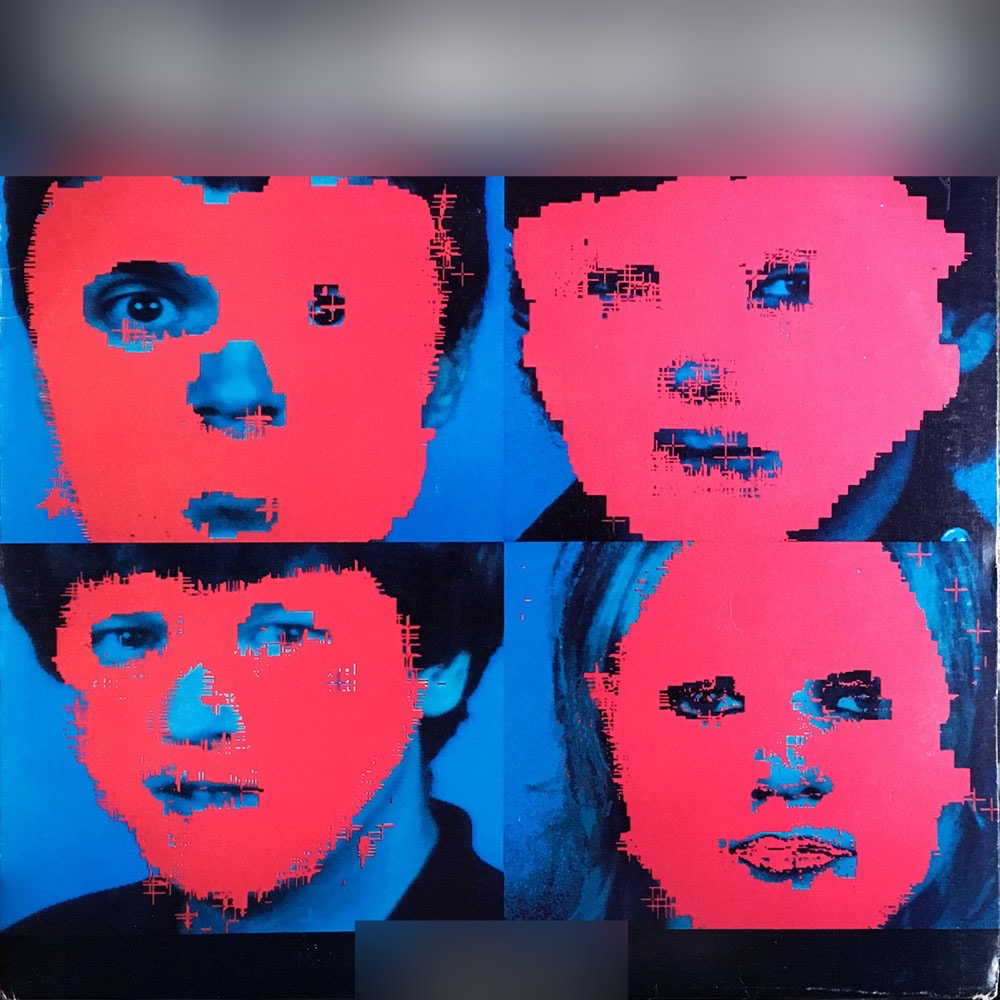
\includegraphics[max width=0.95\textwidth,max height=0.35\textheight]{{Images/remaininlight}.jpeg}
\end{center}
\end{column}
\end{columns}

\visible<2->{
    \begin{columns}[T,totalwidth=\linewidth]
    \begin{column}{0.32\linewidth}
    \begin{block}{Answer}
    \emph{Remain in Light} (The Talking Heads)
    \end{block}
    \end{column}
    \begin{column}{0.65\linewidth}
    \begin{center}
    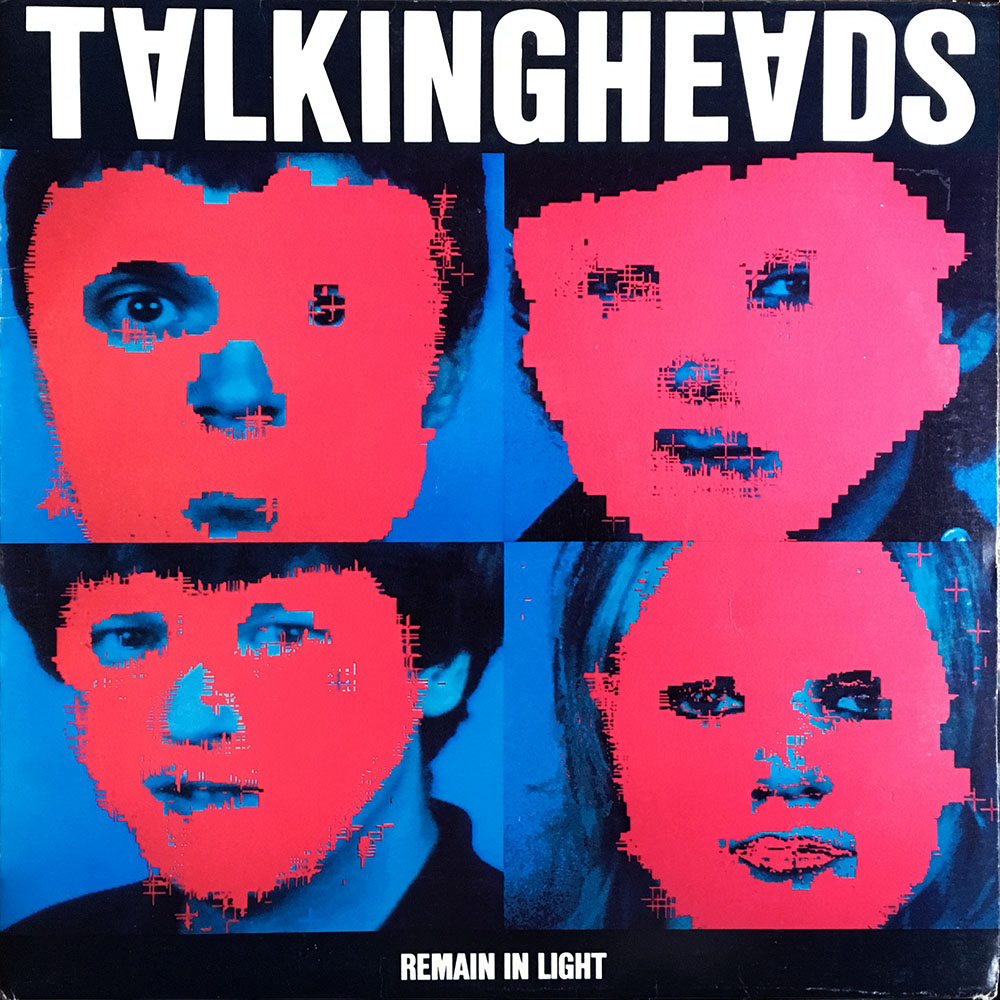
\includegraphics[max width=0.95\textwidth,
        max height=0.38\textheight]{{Images/remaininlightanswer}.jpeg}
    \end{center}
    \end{column}
    \end{columns}
}
\end{frame}
\begin{frame}[t]{Round 1 --- Album by Album Art --- \mbox{Answer 10}}
% \vspace{0.5em}
\begin{columns}[T,totalwidth=\linewidth]
\begin{column}{0.32\linewidth}
\begin{block}{Question}
Name the album.
\end{block}
\end{column}
\begin{column}{0.65\linewidth}
\begin{center}
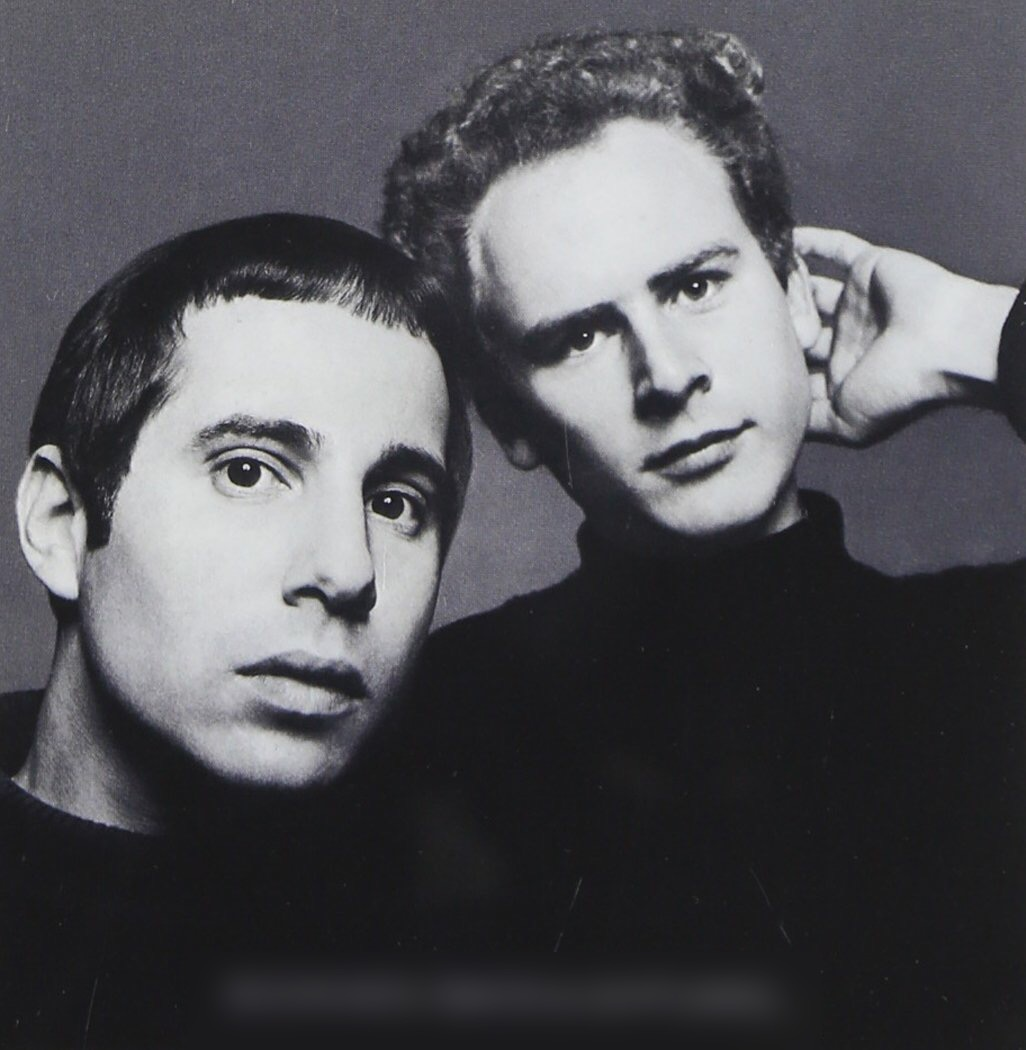
\includegraphics[max width=0.95\textwidth,max height=0.35\textheight]{{Images/bookends}.jpeg}
\end{center}
\end{column}
\end{columns}

\visible<2->{
    \begin{columns}[T,totalwidth=\linewidth]
    \begin{column}{0.32\linewidth}
    \begin{block}{Answer}
    \emph{Bookends} (Simon and Garfunkel)
    \end{block}
    \end{column}
    \begin{column}{0.65\linewidth}
    \begin{center}
    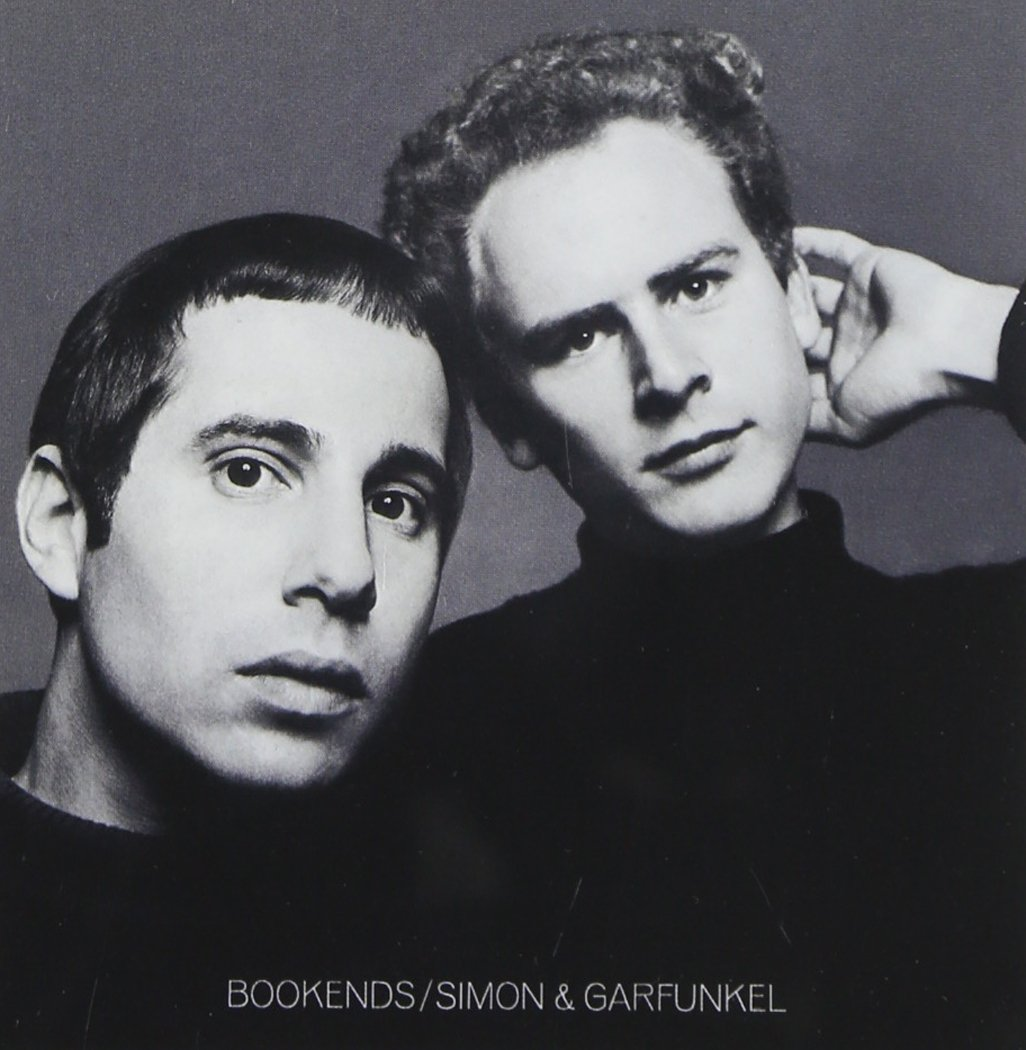
\includegraphics[max width=0.95\textwidth,
        max height=0.38\textheight]{{Images/bookendsanswer}.jpeg}
    \end{center}
    \end{column}
    \end{columns}
}
\end{frame}
\def\thisSectionName{France}
\section{Round 2}
\subsection*{Q1}
\begin{frame}[t]{Round 2 --- France --- \mbox{Question 1}}
% \vspace{0.5em}
\begin{block}{Question}
What is the part of the Mediterranean coast of France that includes Nice, Cannes, and St.\ Tropez called? 
\end{block}
\end{frame}
\subsection*{Q2}
\begin{frame}[t]{Round 2 --- France --- \mbox{Question 2}}
% \vspace{0.5em}
\begin{block}{Question}
Within 5 million, what is the population of France?
\end{block}
\end{frame}
\subsection*{Q3}
\begin{frame}[t]{Round 2 --- France --- \mbox{Question 3}}
% \vspace{0.5em}
\begin{block}{Question}
What square (``place'') in Paris has a giant sundial at its center?
\end{block}
\end{frame}
\subsection*{Q4}
\begin{frame}[t]{Round 2 --- France --- \mbox{Question 4}}
% \vspace{0.5em}
\begin{block}{Question}
How many arrondissements does Paris have?
\end{block}
\end{frame}
\subsection*{Q5}
\begin{frame}[t]{Round 2 --- France --- \mbox{Question 5}}
% \vspace{0.5em}
\begin{block}{Question}
What city is generally regarded as the culinary capital of France?
\end{block}
\end{frame}
\subsection*{Q6}
\begin{frame}[t]{Round 2 --- France --- \mbox{Question 6}}
% \vspace{0.5em}
\begin{block}{Question}
What is the highest mountain in France?
\end{block}
\end{frame}
\subsection*{Q7}
\begin{frame}[t]{Round 2 --- France --- \mbox{Question 7}}
% \vspace{0.5em}
\begin{block}{Question}
In what order do the French refer to the colors of their flag (which are red, white and blue)?
\end{block}
\end{frame}
\subsection*{Q8}
\begin{frame}[t]{Round 2 --- France --- \mbox{Question 8}}
% \vspace{0.5em}
\begin{block}{Question}
What is the name of the French armed force that is made up of non-French citizens?
\end{block}
\end{frame}
\subsection*{Q9}
\begin{frame}[t]{Round 2 --- France --- \mbox{Question 9}}
% \vspace{0.5em}
\begin{block}{Question}
What mountain range forms a natural boundary between France and Spain?
\end{block}
\end{frame}
\subsection*{Q10}
\begin{frame}[t]{Round 2 --- France --- \mbox{Question 10}}
% \vspace{0.5em}
\begin{block}{Question}
What year did the French Revolution (the one that involved the storming of the Bastille) begin?
\end{block}
\end{frame}
\subsection{Answers}
\begin{frame}[t]{Round 2 --- France --- \mbox{Answer 1}}
% \vspace{0.5em}
\begin{block}{Question}
What is the part of the Mediterranean coast of France that includes Nice, Cannes, and St.\ Tropez called? 
\end{block}

\visible<2->{
    \begin{columns}[T,totalwidth=\linewidth]
    \begin{column}{0.32\linewidth}
    \begin{block}{Answer}
    The Riviera or la Côte d'Azur
    \end{block}
    \end{column}
    \begin{column}{0.65\linewidth}
    \begin{center}
    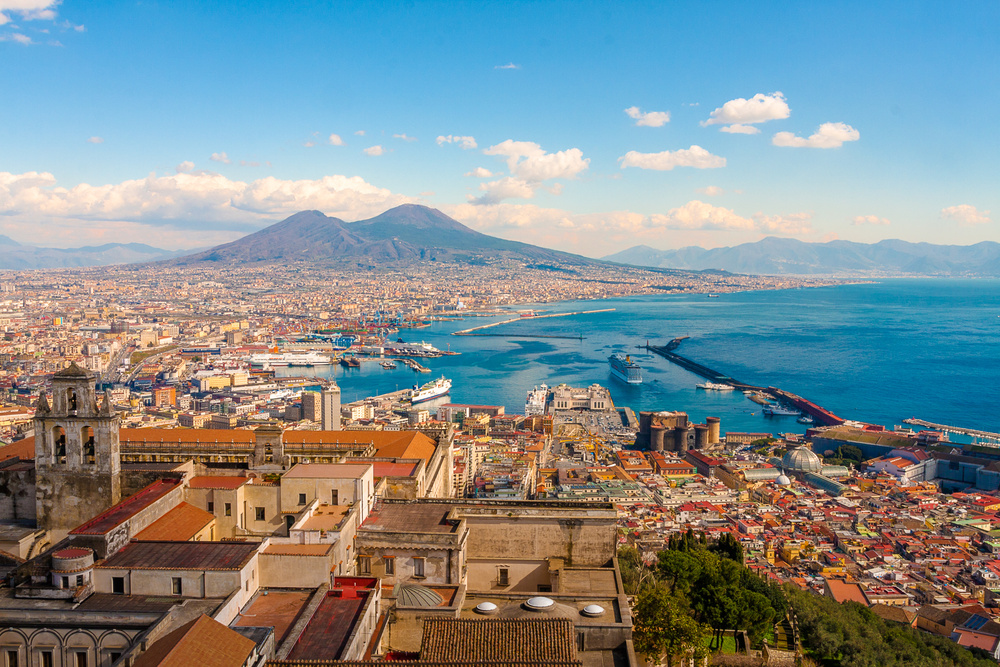
\includegraphics[max width=0.95\textwidth,
        max height=0.50000\textheight]{{Images/riviera}.jpg}
    \end{center}
    \end{column}
    \end{columns}
}
\end{frame}
\begin{frame}[t]{Round 2 --- France --- \mbox{Answer 2}}
% \vspace{0.5em}
\begin{block}{Question}
Within 5 million, what is the population of France?
\end{block}

\visible<2->{
    \begin{columns}[T,totalwidth=\linewidth]
    \begin{column}{0.32\linewidth}
    \begin{block}{Answer}
    Approximately 67 million (we will accept 62 million to 72 million)
    \end{block}
    \end{column}
    \begin{column}{0.65\linewidth}
    \begin{center}
    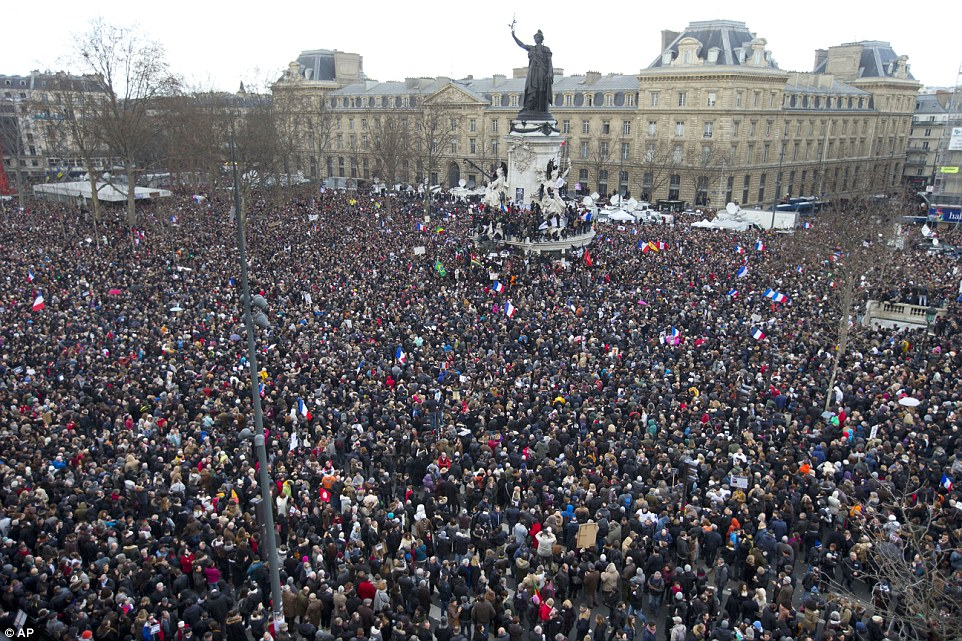
\includegraphics[max width=0.95\textwidth,
        max height=0.54000\textheight]{{Images/francepop}.jpg}
    \end{center}
    \end{column}
    \end{columns}
}
\end{frame}
\begin{frame}[t]{Round 2 --- France --- \mbox{Answer 3}}
% \vspace{0.5em}
\begin{block}{Question}
What square (``place'') in Paris has a giant sundial at its center?
\end{block}

\visible<2->{
    \begin{columns}[T,totalwidth=\linewidth]
    \begin{column}{0.32\linewidth}
    \begin{block}{Answer}
    Place de la Concorde
    \end{block}
    \end{column}
    \begin{column}{0.65\linewidth}
    \begin{center}
    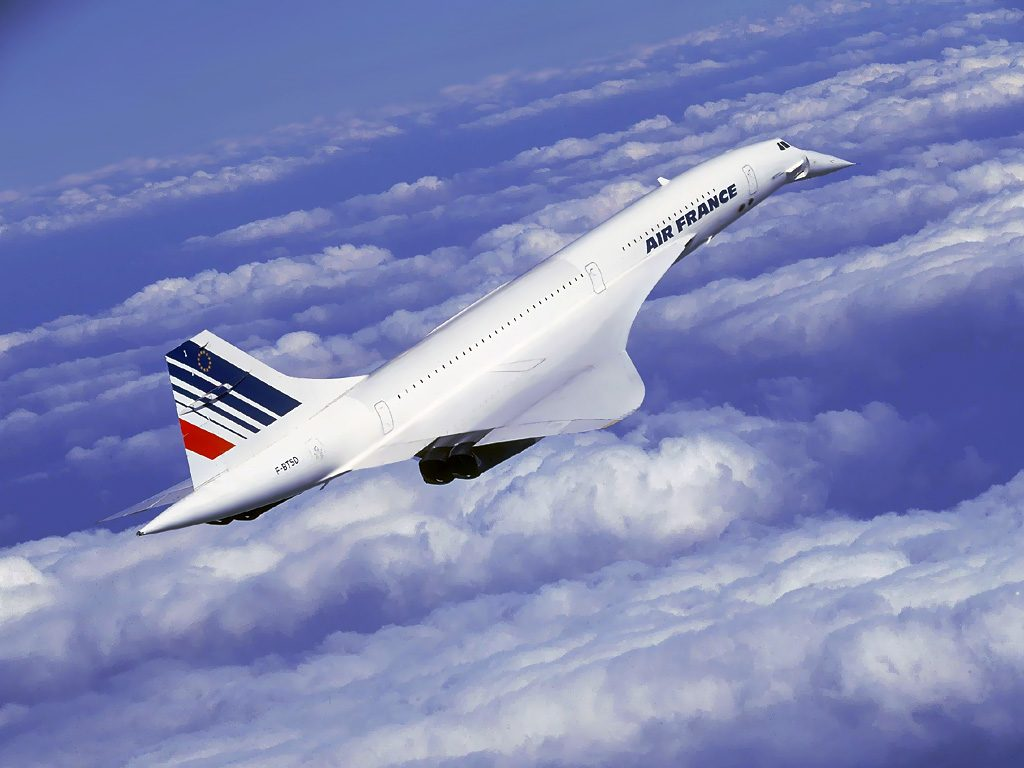
\includegraphics[max width=0.95\textwidth,
        max height=0.54000\textheight]{{Images/concorde}.jpg}
    \end{center}
    \end{column}
    \end{columns}
}
\end{frame}
\begin{frame}[t]{Round 2 --- France --- \mbox{Answer 4}}
% \vspace{0.5em}
\begin{block}{Question}
How many arrondissements does Paris have?
\end{block}

\visible<2->{
    \begin{columns}[T,totalwidth=\linewidth]
    \begin{column}{0.32\linewidth}
    \begin{block}{Answer}
    20
    \end{block}
    \end{column}
    \begin{column}{0.65\linewidth}
    \begin{center}
    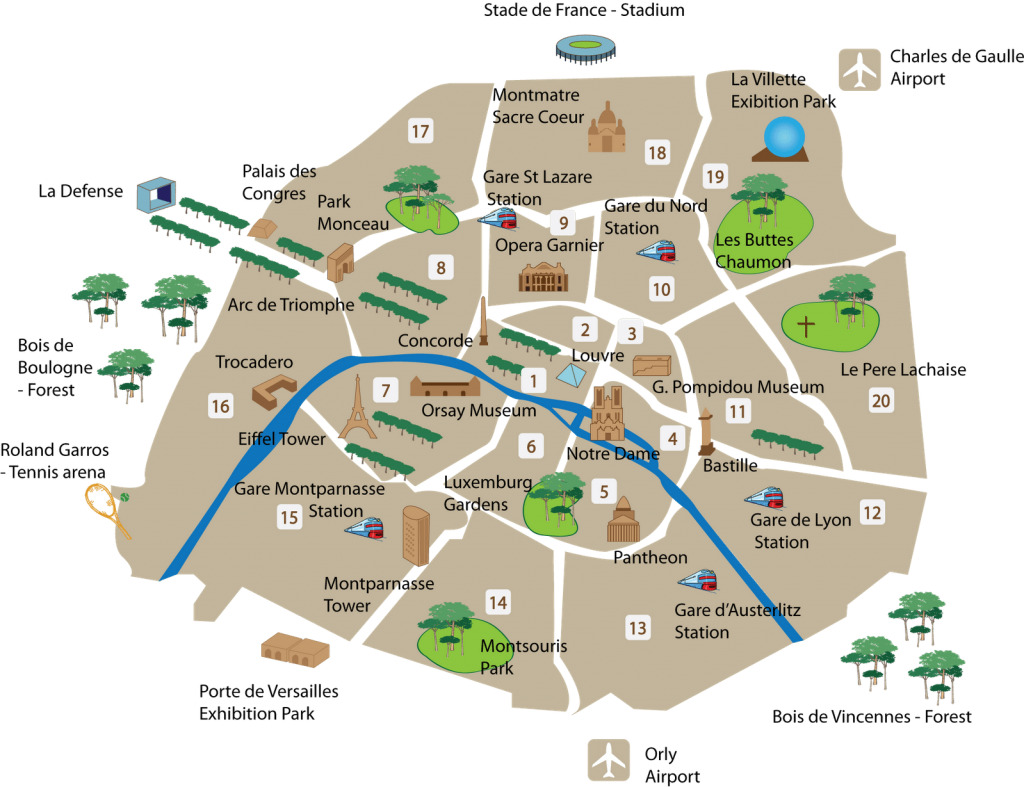
\includegraphics[max width=0.95\textwidth,
        max height=0.58000\textheight]{{Images/arrondissement}.jpg}
    \end{center}
    \end{column}
    \end{columns}
}
\end{frame}
\begin{frame}[t]{Round 2 --- France --- \mbox{Answer 5}}
% \vspace{0.5em}
\begin{block}{Question}
What city is generally regarded as the culinary capital of France?
\end{block}

\visible<2->{
    \begin{columns}[T,totalwidth=\linewidth]
    \begin{column}{0.32\linewidth}
    \begin{block}{Answer}
    Lyon
    \end{block}
    \end{column}
    \begin{column}{0.65\linewidth}
    \begin{center}
    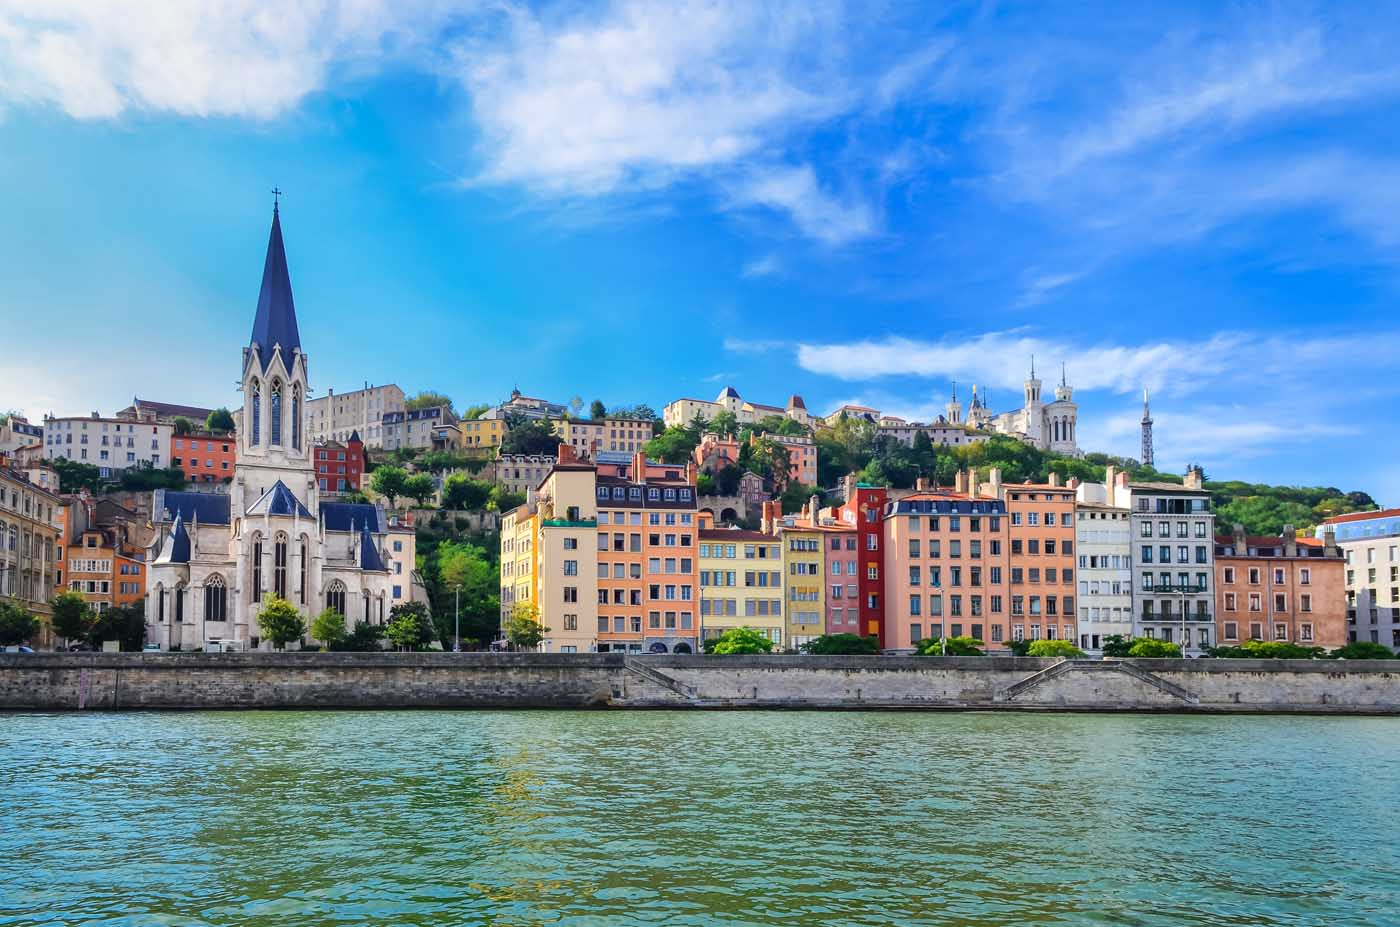
\includegraphics[max width=0.95\textwidth,
        max height=0.54000\textheight]{{Images/lyon}.jpg}
    \end{center}
    \end{column}
    \end{columns}
}
\end{frame}
\begin{frame}[t]{Round 2 --- France --- \mbox{Answer 6}}
% \vspace{0.5em}
\begin{block}{Question}
What is the highest mountain in France?
\end{block}

\visible<2->{
    \begin{columns}[T,totalwidth=\linewidth]
    \begin{column}{0.32\linewidth}
    \begin{block}{Answer}
    Mont Blanc (15,774 feet / 4,810m)
    \end{block}
    \end{column}
    \begin{column}{0.65\linewidth}
    \begin{center}
    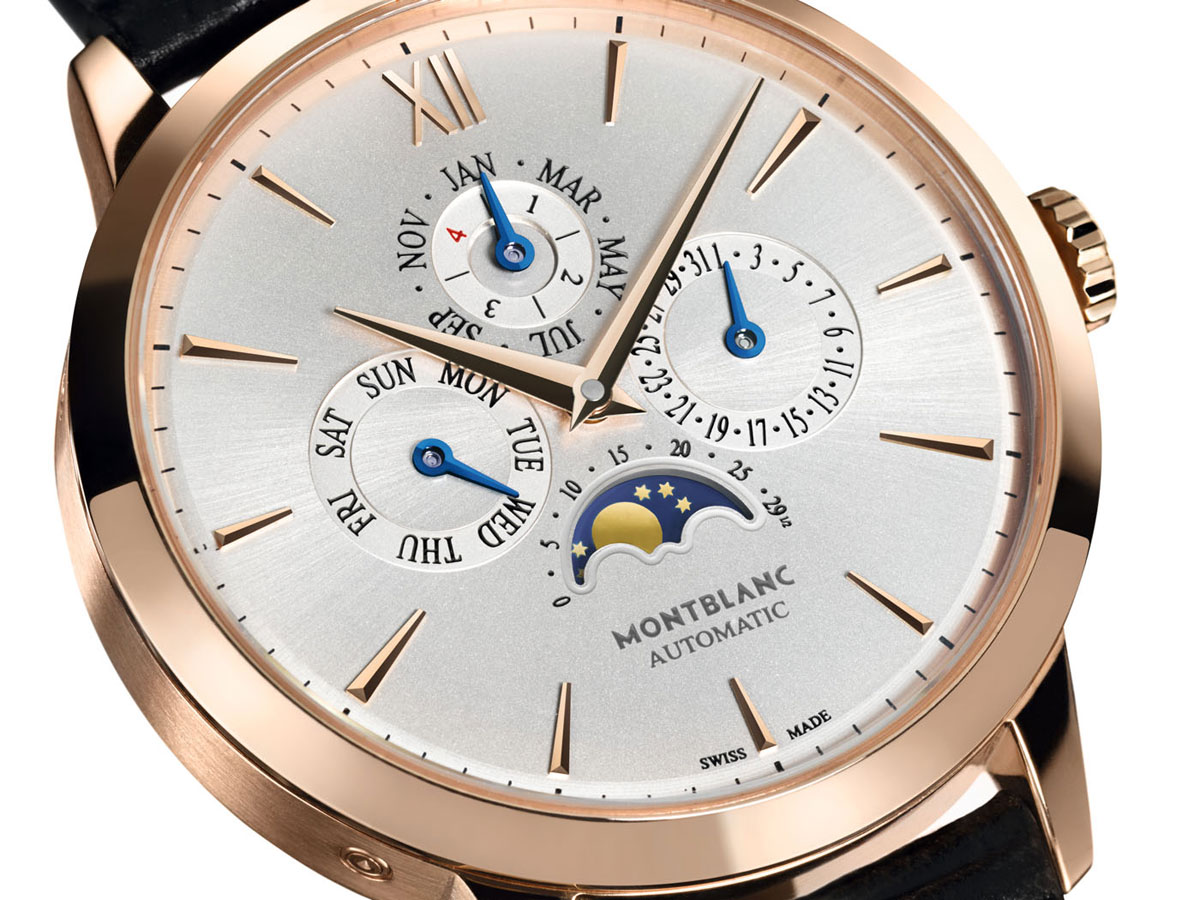
\includegraphics[max width=0.95\textwidth,
        max height=0.58000\textheight]{{Images/montblanc}.jpg}
    \end{center}
    \end{column}
    \end{columns}
}
\end{frame}
\begin{frame}[t]{Round 2 --- France --- \mbox{Answer 7}}
% \vspace{0.5em}
\begin{block}{Question}
In what order do the French refer to the colors of their flag (which are red, white and blue)?
\end{block}

\visible<2->{
    \begin{columns}[T,totalwidth=\linewidth]
    \begin{column}{0.32\linewidth}
    \begin{block}{Answer}
    Blue, white and red
    \end{block}
    \end{column}
    \begin{column}{0.65\linewidth}
    \begin{center}
    
\includegraphics[max width=0.95\textwidth,
        max height=0.54000\textheight]{{Images/frenchflag}.png}
    \end{center}
    \end{column}
    \end{columns}
}
\end{frame}
\begin{frame}[t]{Round 2 --- France --- \mbox{Answer 8}}
% \vspace{0.5em}
\begin{block}{Question}
What is the name of the French armed force that is made up of non-French citizens?
\end{block}

\visible<2->{
    \begin{columns}[T,totalwidth=\linewidth]
    \begin{column}{0.32\linewidth}
    \begin{block}{Answer}
    The Foreign Legion
    \end{block}
    \end{column}
    \begin{column}{0.65\linewidth}
    \begin{center}
    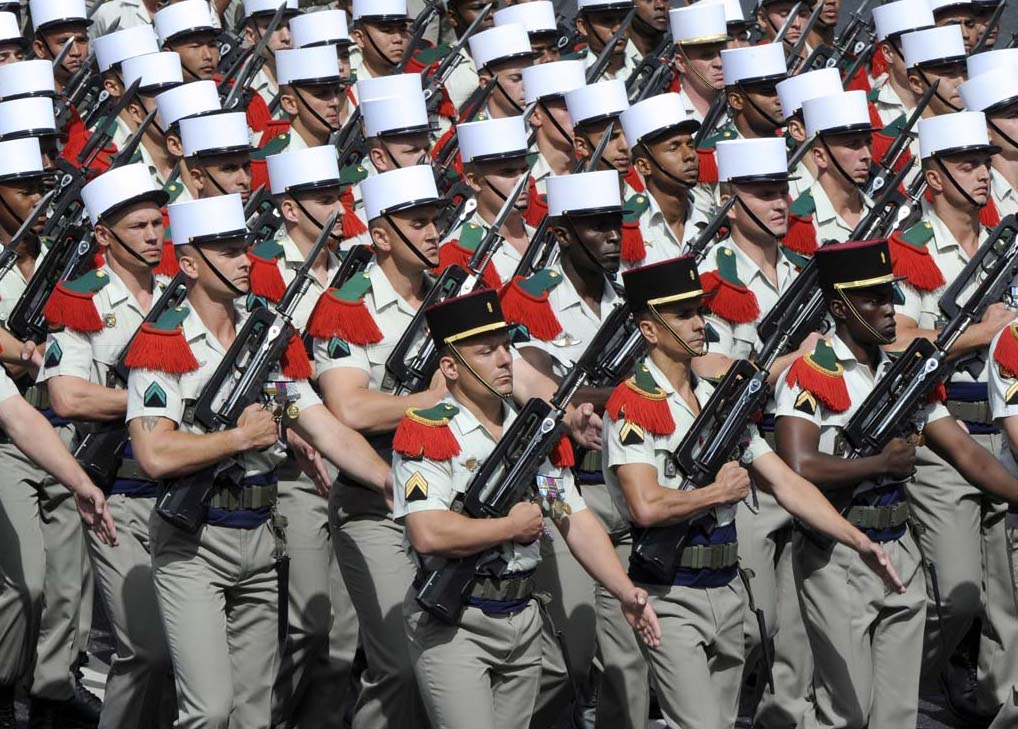
\includegraphics[max width=0.95\textwidth,
        max height=0.54000\textheight]{{Images/foreignlegion}.jpg}
    \end{center}
    \end{column}
    \end{columns}
}
\end{frame}
\begin{frame}[t]{Round 2 --- France --- \mbox{Answer 9}}
% \vspace{0.5em}
\begin{block}{Question}
What mountain range forms a natural boundary between France and Spain?
\end{block}

\visible<2->{
    \begin{columns}[T,totalwidth=\linewidth]
    \begin{column}{0.32\linewidth}
    \begin{block}{Answer}
    The Pyrenees
    \end{block}
    \end{column}
    \begin{column}{0.65\linewidth}
    \begin{center}
    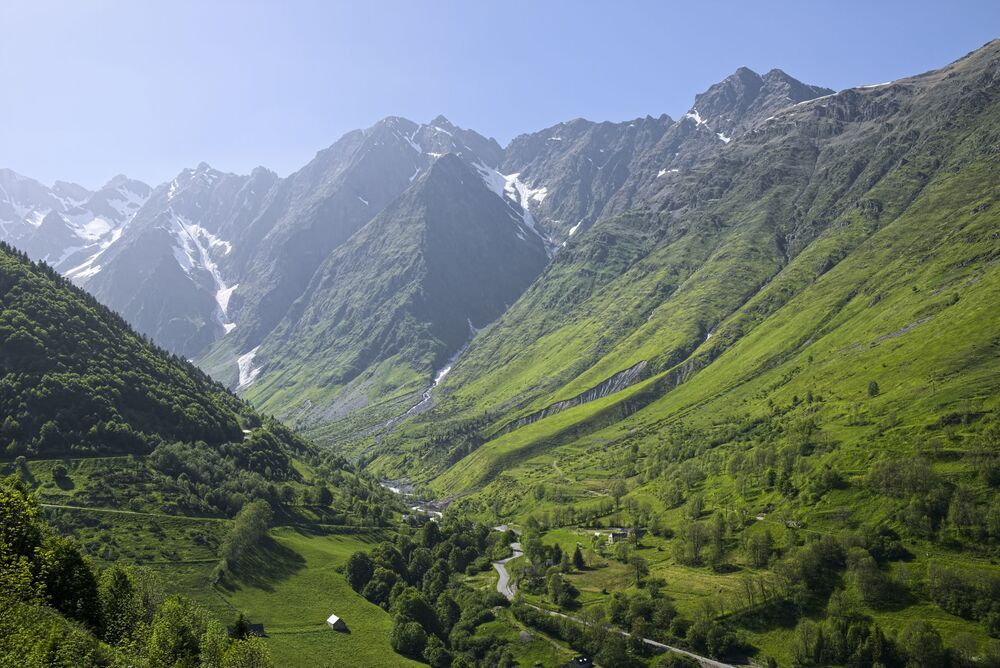
\includegraphics[max width=0.95\textwidth,
        max height=0.54000\textheight]{{Images/pyrenees}.jpg}
    \end{center}
    \end{column}
    \end{columns}
}
\end{frame}
\begin{frame}[t]{Round 2 --- France --- \mbox{Answer 10}}
% \vspace{0.5em}
\begin{block}{Question}
What year did the French Revolution (the one that involved the storming of the Bastille) begin?
\end{block}

\visible<2->{
    \begin{columns}[T,totalwidth=\linewidth]
    \begin{column}{0.32\linewidth}
    \begin{block}{Answer}
    1789
    \end{block}
    \end{column}
    \begin{column}{0.65\linewidth}
    \begin{center}
    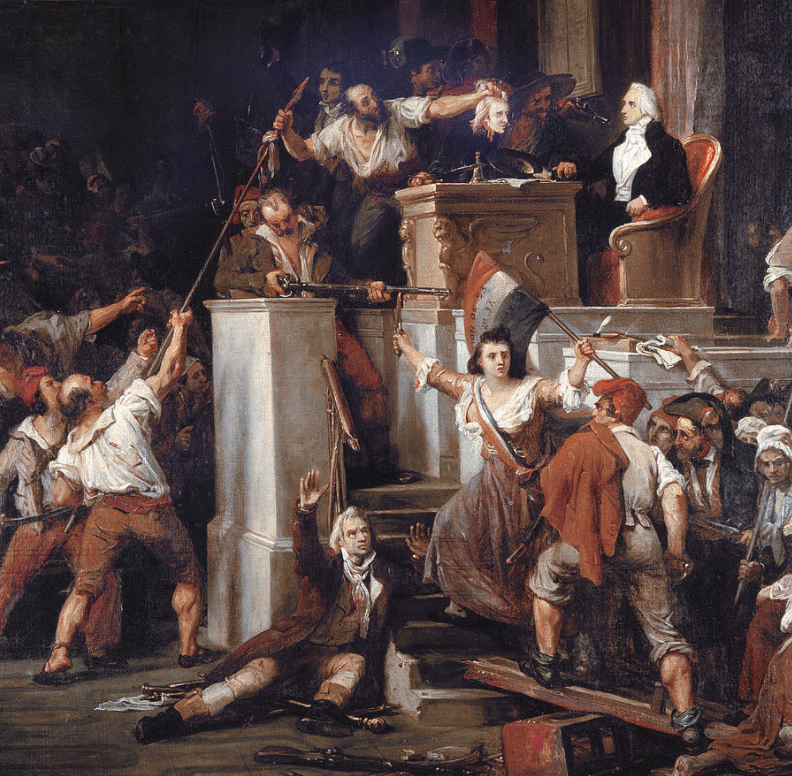
\includegraphics[max width=0.95\textwidth,
        max height=0.54000\textheight]{{Images/frenchrev}.jpg}
    \end{center}
    \end{column}
    \end{columns}
}
\end{frame}
\def\thisSectionName{Airport Codes}
\section{Round 3}
\subsection*{Q1}
\begin{frame}[t]{Round 3 --- Airport Codes --- \mbox{Question 1}}
% \vspace{0.5em}
\begin{block}{Question}
What is the principal city served by LHR\@?
\end{block}
\end{frame}
\subsection*{Q2}
\begin{frame}[t]{Round 3 --- Airport Codes --- \mbox{Question 2}}
% \vspace{0.5em}
\begin{block}{Question}
What is/are the principal city/cities served by DFW\@?
\end{block}
\end{frame}
\subsection*{Q3}
\begin{frame}[t]{Round 3 --- Airport Codes --- \mbox{Question 3}}
% \vspace{0.5em}
\begin{block}{Question}
What is the principal city served by PHX\@?
\end{block}
\end{frame}
\subsection*{Q4}
\begin{frame}[t]{Round 3 --- Airport Codes --- \mbox{Question 4}}
% \vspace{0.5em}
\begin{block}{Question}
What is the principal city served by FRA\@?
\end{block}
\end{frame}
\subsection*{Q5}
\begin{frame}[t]{Round 3 --- Airport Codes --- \mbox{Question 5}}
% \vspace{0.5em}
\begin{block}{Question}
What is the principal city served by FCO\@?
\end{block}
\end{frame}
\subsection*{Q6}
\begin{frame}[t]{Round 3 --- Airport Codes --- \mbox{Question 6}}
% \vspace{0.5em}
\begin{block}{Question}
What is the principal city served by PEK\@?
\end{block}
\end{frame}
\subsection*{Q7}
\begin{frame}[t]{Round 3 --- Airport Codes --- \mbox{Question 7}}
% \vspace{0.5em}
\begin{block}{Question}
What is the principal city served by ORD\@?
\end{block}
\end{frame}
\subsection*{Q8}
\begin{frame}[t]{Round 3 --- Airport Codes --- \mbox{Question 8}}
% \vspace{0.5em}
\begin{block}{Question}
What is the principal city served by CDG\@?
\end{block}
\end{frame}
\subsection*{Q9}
\begin{frame}[t]{Round 3 --- Airport Codes --- \mbox{Question 9}}
% \vspace{0.5em}
\begin{block}{Question}
What is the principal city served by LGA\@?
\end{block}
\end{frame}
\subsection*{Q10}
\begin{frame}[t]{Round 3 --- Airport Codes --- \mbox{Question 10}}
% \vspace{0.5em}
\begin{block}{Question}
What is/are the principal city/cities served by BWI\@?
\end{block}
\end{frame}
\subsection{Answers}
\begin{frame}[t]{Round 3 --- Airport Codes --- \mbox{Answer 1}}
% \vspace{0.5em}
\begin{block}{Question}
What is the principal city served by LHR\@?
\end{block}

\visible<2->{
    \begin{columns}[T,totalwidth=\linewidth]
    \begin{column}{0.32\linewidth}
    \begin{block}{Answer}
    London (London Heathrow Airport)
    \end{block}
    \end{column}
    \begin{column}{0.65\linewidth}
    \begin{center}
    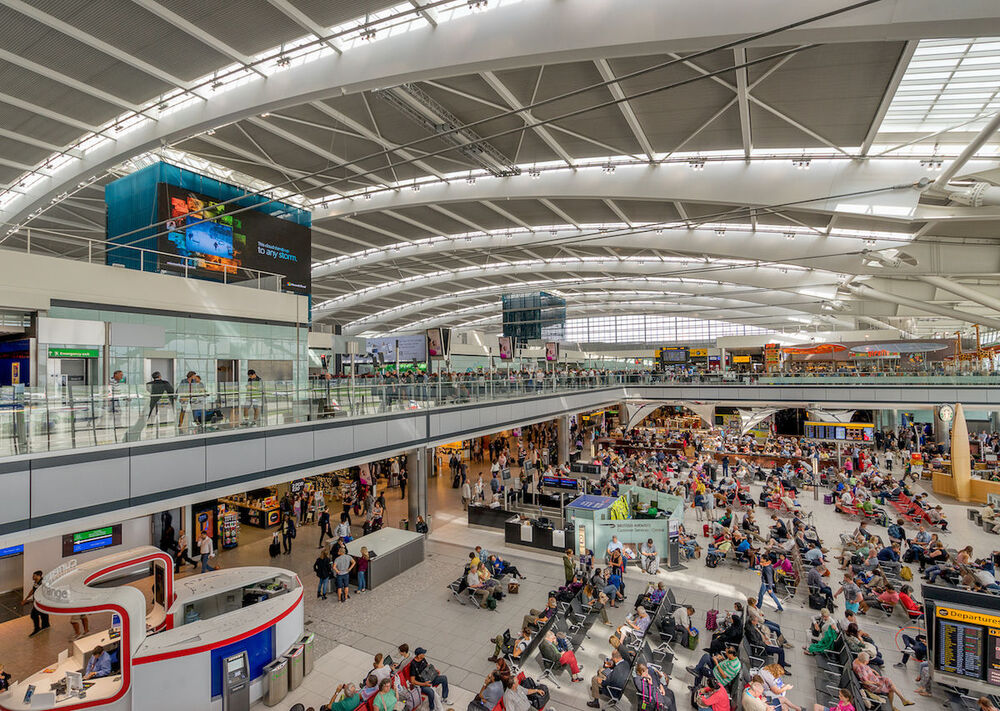
\includegraphics[max width=0.95\textwidth,
        max height=0.58000\textheight]{{Images/heathrow}.jpg}
    \end{center}
    \end{column}
    \end{columns}
}
\end{frame}
\begin{frame}[t]{Round 3 --- Airport Codes --- \mbox{Answer 2}}
% \vspace{0.5em}
\begin{block}{Question}
What is/are the principal city/cities served by DFW\@?
\end{block}

\visible<2->{
    \begin{columns}[T,totalwidth=\linewidth]
    \begin{column}{0.32\linewidth}
    \begin{block}{Answer}
    Dallas or Fort Worth; you only needed one (Dallas/Fort Worth International Airport)
    \end{block}
    \end{column}
    \begin{column}{0.65\linewidth}
    \begin{center}
    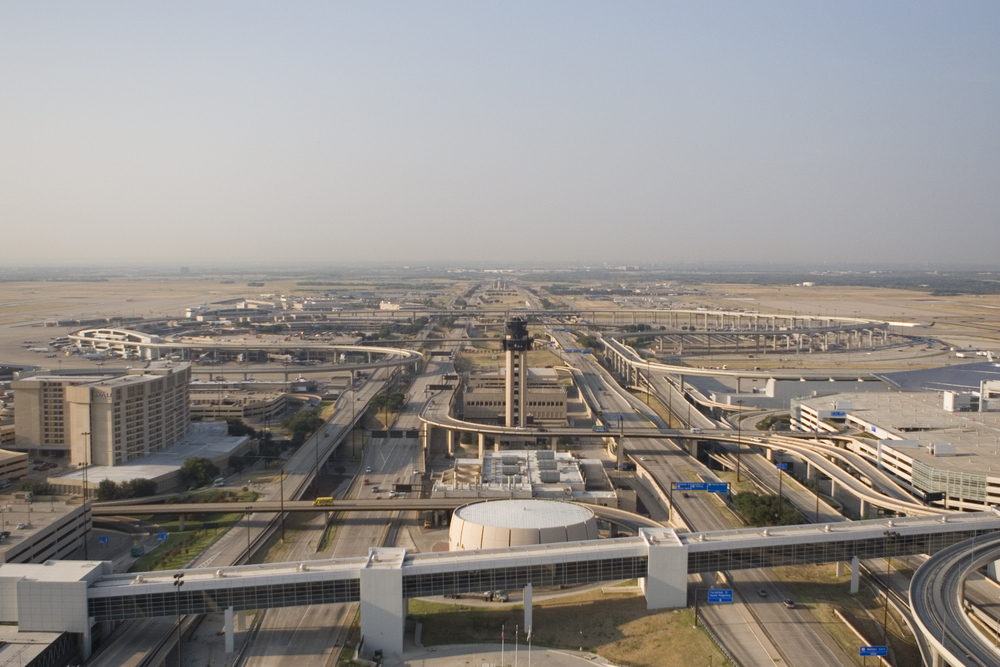
\includegraphics[max width=0.95\textwidth,
        max height=0.54000\textheight]{{Images/dfw}.jpg}
    \end{center}
    \end{column}
    \end{columns}
}
\end{frame}
\begin{frame}[t]{Round 3 --- Airport Codes --- \mbox{Answer 3}}
% \vspace{0.5em}
\begin{block}{Question}
What is the principal city served by PHX\@?
\end{block}

\visible<2->{
    \begin{columns}[T,totalwidth=\linewidth]
    \begin{column}{0.32\linewidth}
    \begin{block}{Answer}
    Phoenix (Phoenix Sky Harbor International Airport)
    \end{block}
    \end{column}
    \begin{column}{0.65\linewidth}
    \begin{center}
    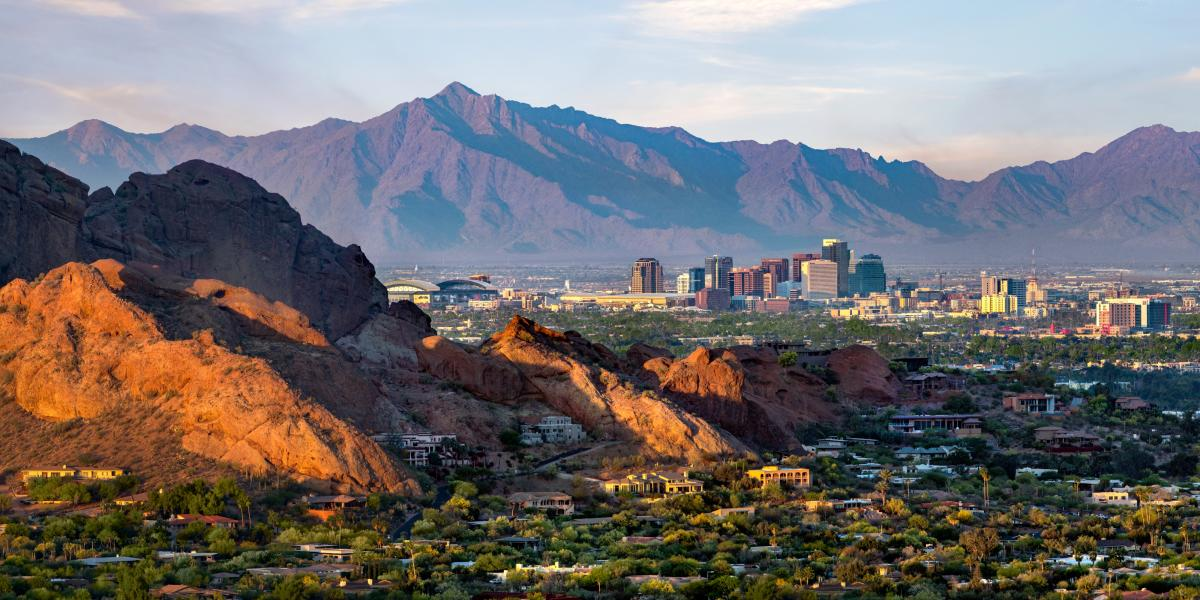
\includegraphics[max width=0.95\textwidth,
        max height=0.58000\textheight]{{Images/phoenix}.jpg}
    \end{center}
    \end{column}
    \end{columns}
}
\end{frame}
\begin{frame}[t]{Round 3 --- Airport Codes --- \mbox{Answer 4}}
% \vspace{0.5em}
\begin{block}{Question}
What is the principal city served by FRA\@?
\end{block}

\visible<2->{
    \begin{columns}[T,totalwidth=\linewidth]
    \begin{column}{0.32\linewidth}
    \begin{block}{Answer}
    Frankfurt (Frankfurt am Main Airport)
    \end{block}
    \end{column}
    \begin{column}{0.65\linewidth}
    \begin{center}
    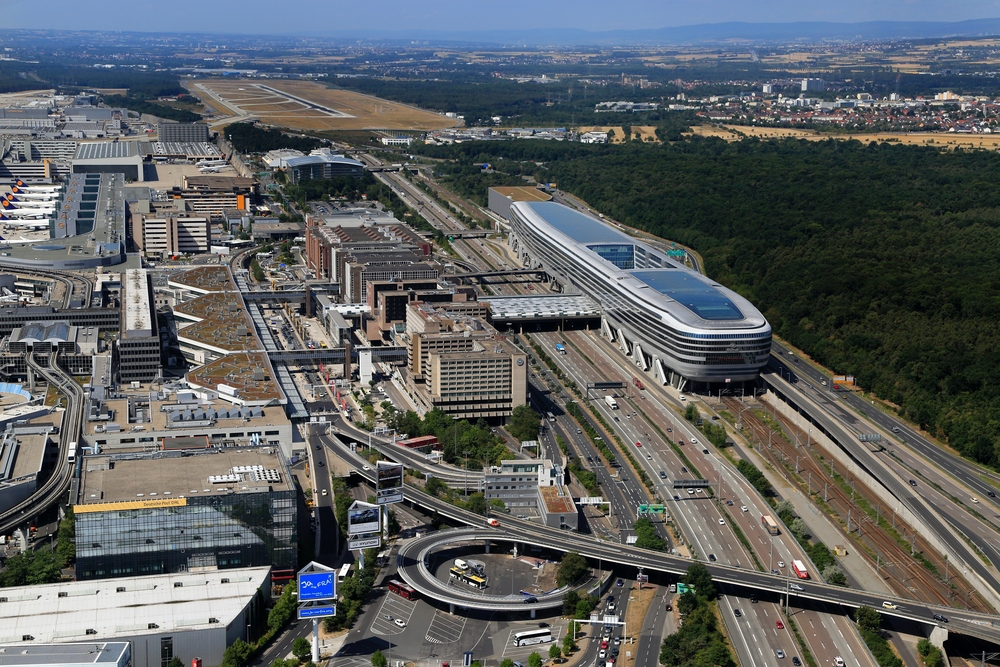
\includegraphics[max width=0.95\textwidth,
        max height=0.58000\textheight]{{Images/fra}.jpg}
    \end{center}
    \end{column}
    \end{columns}
}
\end{frame}
\begin{frame}[t]{Round 3 --- Airport Codes --- \mbox{Answer 5}}
% \vspace{0.5em}
\begin{block}{Question}
What is the principal city served by FCO\@?
\end{block}

\visible<2->{
    \begin{columns}[T,totalwidth=\linewidth]
    \begin{column}{0.32\linewidth}
    \begin{block}{Answer}
    Rome (Rome-Fiumicino International Airport ``Leonardo da Vinci'')
    \end{block}
    \end{column}
    \begin{column}{0.65\linewidth}
    \begin{center}
    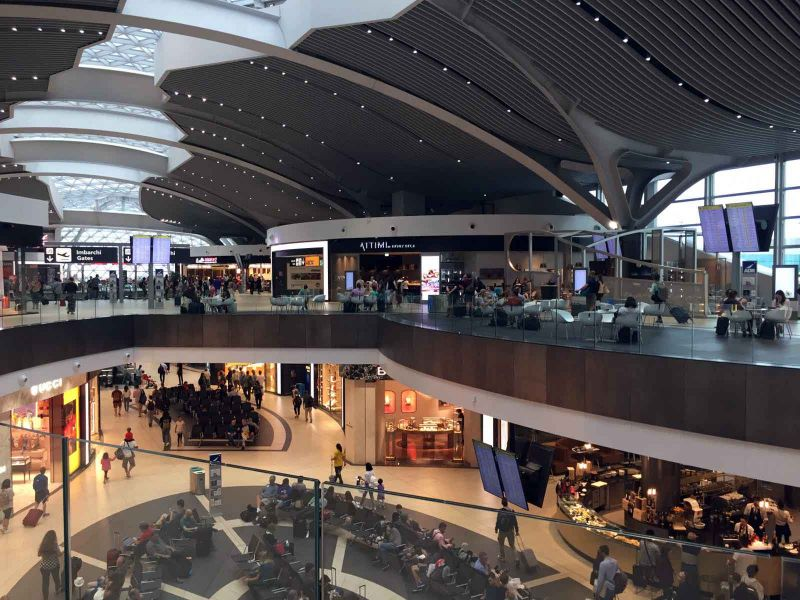
\includegraphics[max width=0.95\textwidth,
        max height=0.58000\textheight]{{Images/fco}.jpg}
    \end{center}
    \end{column}
    \end{columns}
}
\end{frame}
\begin{frame}[t]{Round 3 --- Airport Codes --- \mbox{Answer 6}}
% \vspace{0.5em}
\begin{block}{Question}
What is the principal city served by PEK\@?
\end{block}

\visible<2->{
    \begin{columns}[T,totalwidth=\linewidth]
    \begin{column}{0.32\linewidth}
    \begin{block}{Answer}
    Beijing (Beijing Capital International Airport)
    \end{block}
    \end{column}
    \begin{column}{0.65\linewidth}
    \begin{center}
    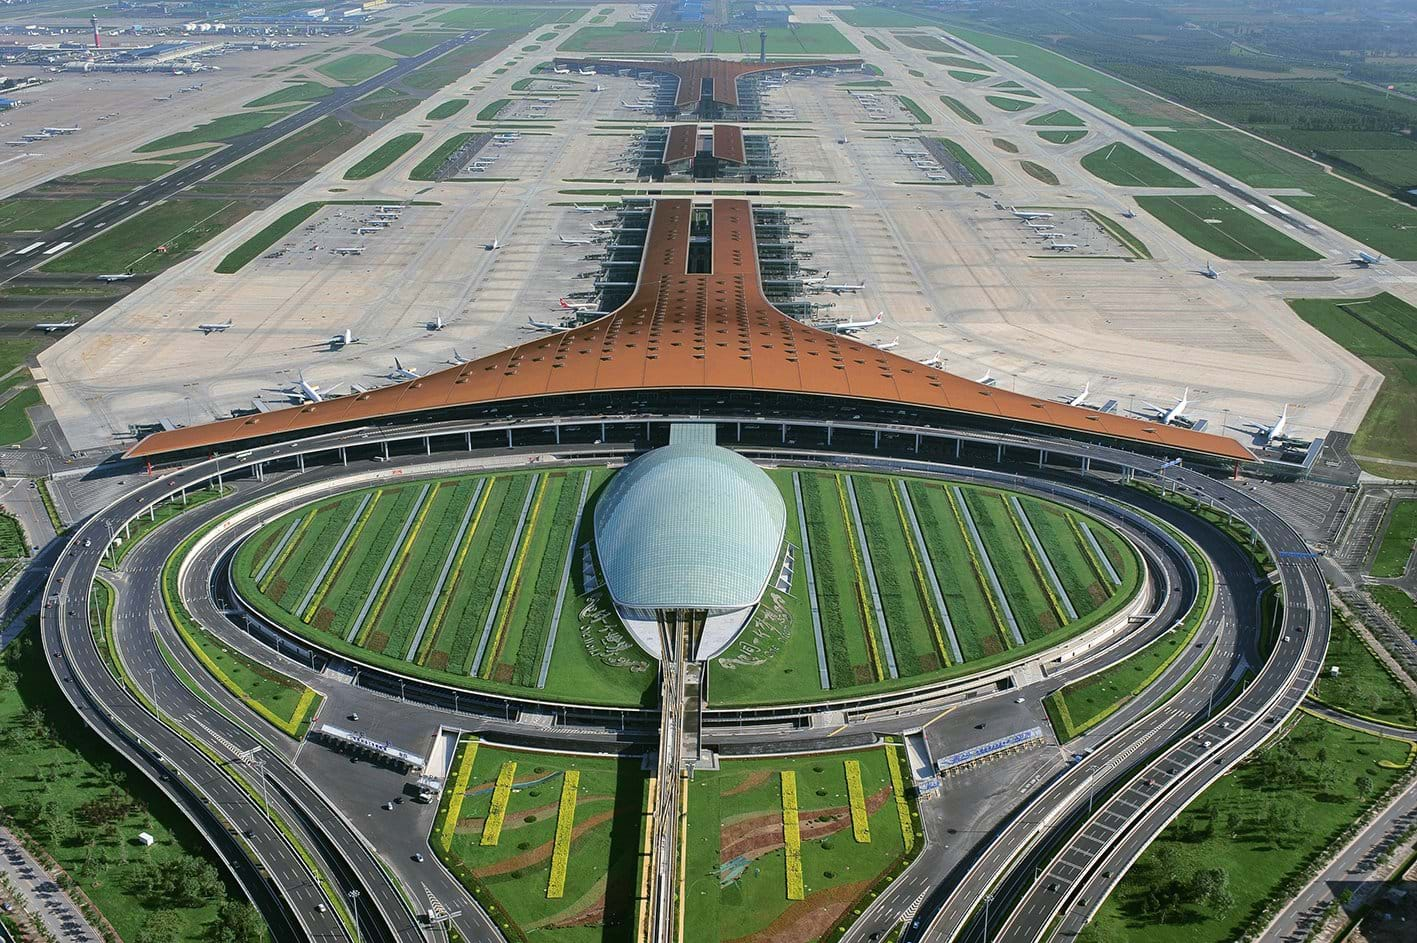
\includegraphics[max width=0.95\textwidth,
        max height=0.58000\textheight]{{Images/pek}.jpg}
    \end{center}
    \end{column}
    \end{columns}
}
\end{frame}
\begin{frame}[t]{Round 3 --- Airport Codes --- \mbox{Answer 7}}
% \vspace{0.5em}
\begin{block}{Question}
What is the principal city served by ORD\@?
\end{block}

\visible<2->{
    \begin{columns}[T,totalwidth=\linewidth]
    \begin{column}{0.32\linewidth}
    \begin{block}{Answer}
    Chicago (Chicago O'Hare International Airport)
    \end{block}
    \end{column}
    \begin{column}{0.65\linewidth}
    \begin{center}
    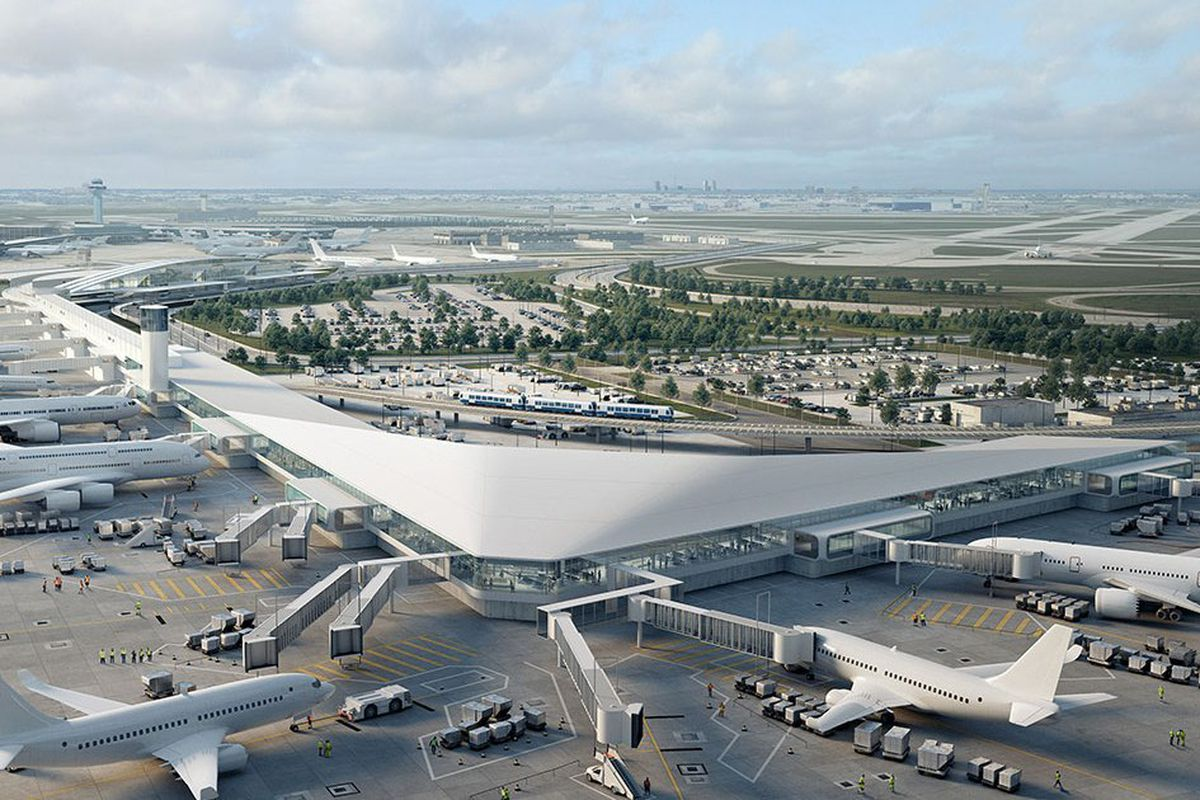
\includegraphics[max width=0.95\textwidth,
        max height=0.58000\textheight]{{Images/ohare}.jpg}
    \end{center}
    \end{column}
    \end{columns}
}
\end{frame}
\begin{frame}[t]{Round 3 --- Airport Codes --- \mbox{Answer 8}}
% \vspace{0.5em}
\begin{block}{Question}
What is the principal city served by CDG\@?
\end{block}

\visible<2->{
    \begin{columns}[T,totalwidth=\linewidth]
    \begin{column}{0.32\linewidth}
    \begin{block}{Answer}
    Paris (Charles de Gaulle Airport)
    \end{block}
    \end{column}
    \begin{column}{0.65\linewidth}
    \begin{center}
    \includegraphics[max width=0.95\textwidth,
        max height=0.58000\textheight]{{Images/cdg}.jpg}
    \end{center}
    \end{column}
    \end{columns}
}
\end{frame}
\begin{frame}[t]{Round 3 --- Airport Codes --- \mbox{Answer 9}}
% \vspace{0.5em}
\begin{block}{Question}
What is the principal city served by LGA\@?
\end{block}

\visible<2->{
    \begin{columns}[T,totalwidth=\linewidth]
    \begin{column}{0.32\linewidth}
    \begin{block}{Answer}
    New York (LaGuardia Airport)
    \end{block}
    \end{column}
    \begin{column}{0.65\linewidth}
    \begin{center}
    \includegraphics[max width=0.95\textwidth,
        max height=0.58000\textheight]{{Images/lga}.jpg}
    \end{center}
    \end{column}
    \end{columns}
}
\end{frame}
\begin{frame}[t]{Round 3 --- Airport Codes --- \mbox{Answer 10}}
% \vspace{0.5em}
\begin{block}{Question}
What is/are the principal city/cities served by BWI\@?
\end{block}

\visible<2->{
    \begin{columns}[T,totalwidth=\linewidth]
    \begin{column}{0.32\linewidth}
    \begin{block}{Answer}
    Baltimore or D.\@C.\@; you only needed one (Baltimore-Washington International Airport)
    \end{block}
    \end{column}
    \begin{column}{0.65\linewidth}
    \begin{center}
    \includegraphics[max width=0.95\textwidth,
        max height=0.54000\textheight]{{Images/bwi}.jpg}
    \end{center}
    \end{column}
    \end{columns}
}
\end{frame}
\def\thisSectionName{Big Dates in History}
\section{Round 4}
\subsection*{Q1}
\begin{frame}[t]{Round 4 --- Big Dates in History --- \mbox{Question 1}}
% \vspace{0.5em}
\begin{block}{Question}
August 28, 1963
\end{block}
\end{frame}
\subsection*{Q2}
\begin{frame}[t]{Round 4 --- Big Dates in History --- \mbox{Question 2}}
% \vspace{0.5em}
\begin{block}{Question}
April 9, 1865
\end{block}
\end{frame}
\subsection*{Q3}
\begin{frame}[t]{Round 4 --- Big Dates in History --- \mbox{Question 3}}
% \vspace{0.5em}
\begin{block}{Question}
May 8, 1945
\end{block}
\end{frame}
\subsection*{Q4}
\begin{frame}[t]{Round 4 --- Big Dates in History --- \mbox{Question 4}}
% \vspace{0.5em}
\begin{block}{Question}
December 25, 800
\end{block}
\end{frame}
\subsection*{Q5}
\begin{frame}[t]{Round 4 --- Big Dates in History --- \mbox{Question 5}}
% \vspace{0.5em}
\begin{block}{Question}
June 8, 1215
\end{block}
\end{frame}
\subsection*{Q6}
\begin{frame}[t]{Round 4 --- Big Dates in History --- \mbox{Question 6}}
% \vspace{0.5em}
\begin{block}{Question}
June 6, 1944
\end{block}
\end{frame}
\subsection*{Q7}
\begin{frame}[t]{Round 4 --- Big Dates in History --- \mbox{Question 7}}
% \vspace{0.5em}
\begin{block}{Question}
October 19, 1781
\end{block}
\end{frame}
\subsection*{Q8}
\begin{frame}[t]{Round 4 --- Big Dates in History --- \mbox{Question 8}}
% \vspace{0.5em}
\begin{block}{Question}
March 8, 1917
\end{block}
\end{frame}
\subsection*{Q9}
\begin{frame}[t]{Round 4 --- Big Dates in History --- \mbox{Question 9}}
% \vspace{0.5em}
\begin{block}{Question}
November 11, 1918
\end{block}
\end{frame}
\subsection*{Q10}
\begin{frame}[t]{Round 4 --- Big Dates in History --- \mbox{Question 10}}
% \vspace{0.5em}
\begin{block}{Question}
March 15, 44 BCE
\end{block}
\end{frame}
\subsection{Answers}
\begin{frame}[t]{Round 4 --- Big Dates in History --- \mbox{Answer 1}}
% \vspace{0.5em}
\begin{block}{Question}
August 28, 1963
\end{block}

\visible<2->{
    \begin{columns}[T,totalwidth=\linewidth]
    \begin{column}{0.32\linewidth}
    \begin{block}{Answer}
    March on Washington/Martin Luther King delivers ``I Have a Dream'' Speech
    \end{block}
    \end{column}
    \begin{column}{0.65\linewidth}
    \begin{center}
    \includegraphics[max width=0.95\textwidth,
        max height=0.58000\textheight]{{Images/mlk}.jpg}
    \end{center}
    \end{column}
    \end{columns}
}
\end{frame}
\begin{frame}[t]{Round 4 --- Big Dates in History --- \mbox{Answer 2}}
% \vspace{0.5em}
\begin{block}{Question}
April 9, 1865
\end{block}

\visible<2->{
    \begin{columns}[T,totalwidth=\linewidth]
    \begin{column}{0.32\linewidth}
    \begin{block}{Answer}
    Lee surrenders to Grant/End of the Civil War
    \end{block}
    \end{column}
    \begin{column}{0.65\linewidth}
    \begin{center}
    \includegraphics[max width=0.95\textwidth,
        max height=0.58000\textheight]{{Images/lee}.jpg}
    \end{center}
    \end{column}
    \end{columns}
}
\end{frame}
\begin{frame}[t]{Round 4 --- Big Dates in History --- \mbox{Answer 3}}
% \vspace{0.5em}
\begin{block}{Question}
May 8, 1945
\end{block}

\visible<2->{
    \begin{columns}[T,totalwidth=\linewidth]
    \begin{column}{0.32\linewidth}
    \begin{block}{Answer}
    V-E Day/Victory in Europe Day
    \end{block}
    \end{column}
    \begin{column}{0.65\linewidth}
    \begin{center}
    \includegraphics[max width=0.95\textwidth,
        max height=0.58000\textheight]{{Images/veday}.jpg}
    \end{center}
    \end{column}
    \end{columns}
}
\end{frame}
\begin{frame}[t]{Round 4 --- Big Dates in History --- \mbox{Answer 4}}
% \vspace{0.5em}
\begin{block}{Question}
December 25, 800
\end{block}

\visible<2->{
    \begin{columns}[T,totalwidth=\linewidth]
    \begin{column}{0.32\linewidth}
    \begin{block}{Answer}
    Charlemagne crowned Roman Emperor (precursor to the Holy Roman Emperor)
    \end{block}
    \end{column}
    \begin{column}{0.65\linewidth}
    \begin{center}
    \includegraphics[max width=0.95\textwidth,
        max height=0.58000\textheight]{{Images/charlemagne}.jpg}
    \end{center}
    \end{column}
    \end{columns}
}
\end{frame}
\begin{frame}[t]{Round 4 --- Big Dates in History --- \mbox{Answer 5}}
% \vspace{0.5em}
\begin{block}{Question}
June 8, 1215
\end{block}

\visible<2->{
    \begin{columns}[T,totalwidth=\linewidth]
    \begin{column}{0.32\linewidth}
    \begin{block}{Answer}
    King John signs Magna Carta at Runnymede
    \end{block}
    \end{column}
    \begin{column}{0.65\linewidth}
    \begin{center}
    \includegraphics[max width=0.95\textwidth,
        max height=0.58000\textheight]{{Images/kingjohn}.jpg}
    \end{center}
    \end{column}
    \end{columns}
}
\end{frame}
\begin{frame}[t]{Round 4 --- Big Dates in History --- \mbox{Answer 6}}
% \vspace{0.5em}
\begin{block}{Question}
June 6, 1944
\end{block}

\visible<2->{
    \begin{columns}[T,totalwidth=\linewidth]
    \begin{column}{0.32\linewidth}
    \begin{block}{Answer}
    D-Day/Allied invasion of Normandy
    \end{block}
    \end{column}
    \begin{column}{0.65\linewidth}
    \begin{center}
    \includegraphics[max width=0.95\textwidth,
        max height=0.58000\textheight]{{Images/dday}.jpg}
    \end{center}
    \end{column}
    \end{columns}
}
\end{frame}
\begin{frame}[t]{Round 4 --- Big Dates in History --- \mbox{Answer 7}}
% \vspace{0.5em}
\begin{block}{Question}
October 19, 1781
\end{block}

\visible<2->{
    \begin{columns}[T,totalwidth=\linewidth]
    \begin{column}{0.32\linewidth}
    \begin{block}{Answer}
    Surrender of the British in the Revolutionary War
    \end{block}
    \end{column}
    \begin{column}{0.65\linewidth}
    \begin{center}
    \includegraphics[max width=0.95\textwidth,
        max height=0.58000\textheight]{{Images/revwar}.jpg}
    \end{center}
    \end{column}
    \end{columns}
}
\end{frame}
\begin{frame}[t]{Round 4 --- Big Dates in History --- \mbox{Answer 8}}
% \vspace{0.5em}
\begin{block}{Question}
March 8, 1917
\end{block}

\visible<2->{
    \begin{columns}[T,totalwidth=\linewidth]
    \begin{column}{0.32\linewidth}
    \begin{block}{Answer}
    Start of the Russian Revolution
    \end{block}
    \end{column}
    \begin{column}{0.65\linewidth}
    \begin{center}
    \includegraphics[max width=0.95\textwidth,
        max height=0.58000\textheight]{{Images/russia}.jpg}
    \end{center}
    \end{column}
    \end{columns}
}
\end{frame}
\begin{frame}[t]{Round 4 --- Big Dates in History --- \mbox{Answer 9}}
% \vspace{0.5em}
\begin{block}{Question}
November 11, 1918
\end{block}

\visible<2->{
    \begin{columns}[T,totalwidth=\linewidth]
    \begin{column}{0.32\linewidth}
    \begin{block}{Answer}
    End of WWI
    \end{block}
    \end{column}
    \begin{column}{0.65\linewidth}
    \begin{center}
    \includegraphics[max width=0.95\textwidth,
        max height=0.58000\textheight]{{Images/wwi}.jpg}
    \end{center}
    \end{column}
    \end{columns}
}
\end{frame}
\begin{frame}[t]{Round 4 --- Big Dates in History --- \mbox{Answer 10}}
% \vspace{0.5em}
\begin{block}{Question}
March 15, 44 BCE
\end{block}

\visible<2->{
    \begin{columns}[T,totalwidth=\linewidth]
    \begin{column}{0.32\linewidth}
    \begin{block}{Answer}
    Julius Caesar assassinated
    \end{block}
    \end{column}
    \begin{column}{0.65\linewidth}
    \begin{center}
    \includegraphics[max width=0.95\textwidth,
        max height=0.58000\textheight]{{Images/caesar}.jpg}
    \end{center}
    \end{column}
    \end{columns}
}
\end{frame}
\def\thisSectionName{Gangsters in Fact and Fiction}
\section{Round 5}
\subsection*{Q1}
\begin{frame}[t]{Round 5 --- Gangsters in Fact and Fiction --- \mbox{Question 1}}
% \vspace{0.5em}
\begin{block}{Question}
Testifying before a Senate committee, what gangster said, ``No proof linking me to any criminal conspiracy, whether it is called `Mafia' or `Cosa Nostra' or whatever other name you wish to give,  has ever been made public''?
\end{block}
\end{frame}
\subsection*{Q2}
\begin{frame}[t]{Round 5 --- Gangsters in Fact and Fiction --- \mbox{Question 2}}
% \vspace{0.5em}
\begin{block}{Question}
What was the name of the movie in which the gangster's final words were the rhetorical question ``Mother of mercy, is this the end of Rico?''
\end{block}
\end{frame}
\subsection*{Q3}
\begin{frame}[t]{Round 5 --- Gangsters in Fact and Fiction --- \mbox{Question 3}}
% \vspace{0.5em}
\begin{block}{Question}
A gangster went to Umberto's Clam House in NYC's Little Italy on April 7, 1972 and found not spaghetti alle vongole but death on the menu.  Who was he?
\end{block}
\end{frame}
\subsection*{Q4}
\begin{frame}[t]{Round 5 --- Gangsters in Fact and Fiction --- \mbox{Question 4}}
% \vspace{0.5em}
\begin{block}{Question}
Dining out never seems to go well for gangsters. Which gangster proved on December 16, 1985 that New York City steaks are to die for?
\end{block}
\end{frame}
\subsection*{Q5}
\begin{frame}[t]{Round 5 --- Gangsters in Fact and Fiction --- \mbox{Question 5}}
% \vspace{0.5em}
\begin{block}{Question}
Which gangster said ``Say hello to my little friend?''
\end{block}
\end{frame}
\subsection*{Q6}
\begin{frame}[t]{Round 5 --- Gangsters in Fact and Fiction --- \mbox{Question 6}}
% \vspace{0.5em}
\begin{columns}[T,totalwidth=\linewidth]
\begin{column}{0.32\linewidth}
\begin{block}{Question}
Which gangster was killed by authorities as he left the Biograph Theater in Chicago on July 22, 1934?
\end{block}
\end{column}
\begin{column}{0.65\linewidth}
\begin{center}
\includegraphics[max width=0.95\textwidth,max height=0.7\textheight]{{Images/biograph}.jpg}
\end{center}
\end{column}
\end{columns}
\end{frame}
\subsection*{Q7}
\begin{frame}[t]{Round 5 --- Gangsters in Fact and Fiction --- \mbox{Question 7}}
% \vspace{0.5em}
\begin{block}{Question}
In \emph{Goodfellas}, this gangster ended up in the witness protection program.
\end{block}
\end{frame}
\subsection*{Q8}
\begin{frame}[t]{Round 5 --- Gangsters in Fact and Fiction --- \mbox{Question 8}}
% \vspace{0.5em}
\begin{block}{Question}
In \emph{Godfather II}, the character of Hyman Roth is based on which real life gangster? 
\end{block}
\end{frame}
\subsection*{Q9}
\begin{frame}[t]{Round 5 --- Gangsters in Fact and Fiction --- \mbox{Question 9}}
% \vspace{0.5em}
\begin{block}{Question}
This gangster, known as ``the Brain'', is believed to have been involved in fixing the 1919 World Series.
\end{block}
\end{frame}
\subsection*{Q10}
\begin{frame}[t]{Round 5 --- Gangsters in Fact and Fiction --- \mbox{Question 10}}
% \vspace{0.5em}
\begin{block}{Question}
This gangster, who controlled Chicago crime during Prohibition, was ultimately sent to jail for tax evasion.
\end{block}
\end{frame}
\subsection{Answers}
\begin{frame}[t]{Round 5 --- Gangsters in Fact and Fiction --- \mbox{Answer 1}}
% \vspace{0.5em}
\begin{block}{Question}
Testifying before a Senate committee, what gangster said, ``No proof linking me to any criminal conspiracy, whether it is called `Mafia' or `Cosa Nostra' or whatever other name you wish to give,  has ever been made public''?
\end{block}

\visible<2->{
    \begin{columns}[T,totalwidth=\linewidth]
    \begin{column}{0.32\linewidth}
    \begin{block}{Answer}
    Michael Corleone
    \end{block}
    \end{column}
    \begin{column}{0.65\linewidth}
    \begin{center}
    \includegraphics[max width=0.95\textwidth,
        max height=0.42000\textheight]{{Images/corleone}.jpeg}
    \end{center}
    \end{column}
    \end{columns}
}
\end{frame}
\begin{frame}[t]{Round 5 --- Gangsters in Fact and Fiction --- \mbox{Answer 2}}
% \vspace{0.5em}
\begin{block}{Question}
What was the name of the movie in which the gangster's final words were the rhetorical question ``Mother of mercy, is this the end of Rico?''
\end{block}

\visible<2->{
    \begin{columns}[T,totalwidth=\linewidth]
    \begin{column}{0.32\linewidth}
    \begin{block}{Answer}
    \emph{Little Caesar} (not the ``Pizza Pizza'' one)
    \end{block}
    \end{column}
    \begin{column}{0.65\linewidth}
    \begin{center}
    \includegraphics[max width=0.95\textwidth,
        max height=0.50000\textheight]{{Images/littlecaesar}.jpg}
    \end{center}
    \end{column}
    \end{columns}
}
\end{frame}
\begin{frame}[t]{Round 5 --- Gangsters in Fact and Fiction --- \mbox{Answer 3}}
% \vspace{0.5em}
\begin{block}{Question}
A gangster went to Umberto's Clam House in NYC's Little Italy on April 7, 1972 and found not spaghetti alle vongole but death on the menu.  Who was he?
\end{block}

\visible<2->{
    \begin{columns}[T,totalwidth=\linewidth]
    \begin{column}{0.32\linewidth}
    \begin{block}{Answer}
    Crazy Joe Gallo
    \end{block}
    \end{column}
    \begin{column}{0.65\linewidth}
    \begin{center}
    \includegraphics[max width=0.95\textwidth,
        max height=0.46000\textheight]{{Images/crazyjoe}.jpg}
    \end{center}
    \end{column}
    \end{columns}
}
\end{frame}
\begin{frame}[t]{Round 5 --- Gangsters in Fact and Fiction --- \mbox{Answer 4}}
% \vspace{0.5em}
\begin{block}{Question}
Dining out never seems to go well for gangsters. Which gangster proved on December 16, 1985 that New York City steaks are to die for?
\end{block}

\visible<2->{
    \begin{columns}[T,totalwidth=\linewidth]
    \begin{column}{0.32\linewidth}
    \begin{block}{Answer}
    Paul Castellano, killed in front of Sparks Steak House
    \end{block}
    \end{column}
    \begin{column}{0.65\linewidth}
    \begin{center}
    \includegraphics[max width=0.95\textwidth,
        max height=0.50000\textheight]{{Images/castellano}.jpg}
    \end{center}
    \end{column}
    \end{columns}
}
\end{frame}
\begin{frame}[t]{Round 5 --- Gangsters in Fact and Fiction --- \mbox{Answer 5}}
% \vspace{0.5em}
\begin{block}{Question}
Which gangster said ``Say hello to my little friend?''
\end{block}

\visible<2->{
    \begin{columns}[T,totalwidth=\linewidth]
    \begin{column}{0.32\linewidth}
    \begin{block}{Answer}
    Scarface / Tony Montana (Al Pacino version)
    \end{block}
    \end{column}
    \begin{column}{0.65\linewidth}
    \begin{center}
    \includegraphics[max width=0.95\textwidth,
        max height=0.54000\textheight]{{Images/scarface}.jpg}
    \end{center}
    \end{column}
    \end{columns}
}
\end{frame}
\begin{frame}[t]{Round 5 --- Gangsters in Fact and Fiction --- \mbox{Answer 6}}
% \vspace{0.5em}
\begin{columns}[T,totalwidth=\linewidth]
\begin{column}{0.32\linewidth}
\begin{block}{Question}
Which gangster was killed by authorities as he left the Biograph Theater in Chicago on July 22, 1934?
\end{block}
\end{column}
\begin{column}{0.65\linewidth}
\begin{center}
\includegraphics[max width=0.95\textwidth,max height=0.35\textheight]{{Images/biograph}.jpg}
\end{center}
\end{column}
\end{columns}

\visible<2->{
    \begin{columns}[T,totalwidth=\linewidth]
    \begin{column}{0.32\linewidth}
    \begin{block}{Answer}
    John Dillinger
    \end{block}
    \end{column}
    \begin{column}{0.65\linewidth}
    \begin{center}
    \includegraphics[max width=0.95\textwidth,
        max height=0.38\textheight]{{Images/dillinger}.jpg}
    \end{center}
    \end{column}
    \end{columns}
}
\end{frame}
\begin{frame}[t]{Round 5 --- Gangsters in Fact and Fiction --- \mbox{Answer 7}}
% \vspace{0.5em}
\begin{block}{Question}
In \emph{Goodfellas}, this gangster ended up in the witness protection program.
\end{block}

\visible<2->{
    \begin{columns}[T,totalwidth=\linewidth]
    \begin{column}{0.32\linewidth}
    \begin{block}{Answer}
    Henry Hill
    \end{block}
    \end{column}
    \begin{column}{0.65\linewidth}
    \begin{center}
    \includegraphics[max width=0.95\textwidth,
        max height=0.54000\textheight]{{Images/hill}.jpg}
    \end{center}
    \end{column}
    \end{columns}
}
\end{frame}
\begin{frame}[t]{Round 5 --- Gangsters in Fact and Fiction --- \mbox{Answer 8}}
% \vspace{0.5em}
\begin{block}{Question}
In \emph{Godfather II}, the character of Hyman Roth is based on which real life gangster? 
\end{block}

\visible<2->{
    \begin{columns}[T,totalwidth=\linewidth]
    \begin{column}{0.32\linewidth}
    \begin{block}{Answer}
    Meyer Lansky
    \end{block}
    \end{column}
    \begin{column}{0.65\linewidth}
    \begin{center}
    \includegraphics[max width=0.95\textwidth,
        max height=0.54000\textheight]{{Images/lanksy}.jpg}
    \end{center}
    \end{column}
    \end{columns}
}
\end{frame}
\begin{frame}[t]{Round 5 --- Gangsters in Fact and Fiction --- \mbox{Answer 9}}
% \vspace{0.5em}
\begin{block}{Question}
This gangster, known as ``the Brain'', is believed to have been involved in fixing the 1919 World Series.
\end{block}

\visible<2->{
    \begin{columns}[T,totalwidth=\linewidth]
    \begin{column}{0.32\linewidth}
    \begin{block}{Answer}
    Arnold Rothstein
    \end{block}
    \end{column}
    \begin{column}{0.65\linewidth}
    \begin{center}
    \includegraphics[max width=0.95\textwidth,
        max height=0.50000\textheight]{{Images/rothstein}.jpeg}
    \end{center}
    \end{column}
    \end{columns}
}
\end{frame}
\begin{frame}[t]{Round 5 --- Gangsters in Fact and Fiction --- \mbox{Answer 10}}
% \vspace{0.5em}
\begin{block}{Question}
This gangster, who controlled Chicago crime during Prohibition, was ultimately sent to jail for tax evasion.
\end{block}

\visible<2->{
    \begin{columns}[T,totalwidth=\linewidth]
    \begin{column}{0.32\linewidth}
    \begin{block}{Answer}
    Al Capone
    \end{block}
    \end{column}
    \begin{column}{0.65\linewidth}
    \begin{center}
    \includegraphics[max width=0.95\textwidth,
        max height=0.50000\textheight]{{Images/capone}.jpg}
    \end{center}
    \end{column}
    \end{columns}
}
\end{frame}
\def\thisSectionName{Holidays and Observances}
\section{Round 6}
\subsection*{Q1}
\begin{frame}[t]{Round 6 --- Holidays and Observances --- \mbox{Question 1}}
% \vspace{0.5em}
\begin{block}{Question}
What is the holiday celebrated by many  Indians and Indian-Americans on which participants throw colored powder on one another?
\end{block}
\end{frame}
\subsection*{Q2}
\begin{frame}[t]{Round 6 --- Holidays and Observances --- \mbox{Question 2}}
% \vspace{0.5em}
\begin{block}{Question}
What holiday is celebrated in Canada on the second Monday in October?
\end{block}
\end{frame}
\subsection*{Q3}
\begin{frame}[t]{Round 6 --- Holidays and Observances --- \mbox{Question 3}}
% \vspace{0.5em}
\begin{block}{Question}
What offbeat holiday that occurs on January 19th each year might best be observed at a movie theater?
\end{block}
\end{frame}
\subsection*{Q4}
\begin{frame}[t]{Round 6 --- Holidays and Observances --- \mbox{Question 4}}
% \vspace{0.5em}
\begin{block}{Question}
Memorial Day originally honored soldiers who died in which war?
\end{block}
\end{frame}
\subsection*{Q5}
\begin{frame}[t]{Round 6 --- Holidays and Observances --- \mbox{Question 5}}
% \vspace{0.5em}
\begin{block}{Question}
To within three years, in what year was Martin Luther King Jr.\ Day first observed as a national holiday?
\end{block}
\end{frame}
\subsection*{Q6}
\begin{frame}[t]{Round 6 --- Holidays and Observances --- \mbox{Question 6}}
% \vspace{0.5em}
\begin{block}{Question}
Which president made Thanksgiving a national holiday?
\end{block}
\end{frame}
\subsection*{Q7}
\begin{frame}[t]{Round 6 --- Holidays and Observances --- \mbox{Question 7}}
% \vspace{0.5em}
\begin{block}{Question}
What date is flag day?
\end{block}
\end{frame}
\subsection*{Q8}
\begin{frame}[t]{Round 6 --- Holidays and Observances --- \mbox{Question 8}}
% \vspace{0.5em}
\begin{block}{Question}
On which offbeat holiday that occurs on September 19th each year should you sound like Blackbeard?
\end{block}
\end{frame}
\subsection*{Q9}
\begin{frame}[t]{Round 6 --- Holidays and Observances --- \mbox{Question 9}}
% \vspace{0.5em}
\begin{block}{Question}
This holiday that occurs on June 19th celebrates the freeing in Texas of the last American slaves to be freed.
\end{block}
\end{frame}
\subsection*{Q10}
\begin{frame}[t]{Round 6 --- Holidays and Observances --- \mbox{Question 10}}
% \vspace{0.5em}
\begin{block}{Question}
What is the best-selling Christmas song of all time?
\end{block}
\end{frame}
\subsection{Answers}
\begin{frame}[t]{Round 6 --- Holidays and Observances --- \mbox{Answer 1}}
% \vspace{0.5em}
\begin{block}{Question}
What is the holiday celebrated by many  Indians and Indian-Americans on which participants throw colored powder on one another?
\end{block}

\visible<2->{
    \begin{columns}[T,totalwidth=\linewidth]
    \begin{column}{0.32\linewidth}
    \begin{block}{Answer}
    Holi
    \end{block}
    \end{column}
    \begin{column}{0.65\linewidth}
    \begin{center}
    \includegraphics[max width=0.95\textwidth,
        max height=0.50000\textheight]{{Images/holi}.jpg}
    \end{center}
    \end{column}
    \end{columns}
}
\end{frame}
\begin{frame}[t]{Round 6 --- Holidays and Observances --- \mbox{Answer 2}}
% \vspace{0.5em}
\begin{block}{Question}
What holiday is celebrated in Canada on the second Monday in October?
\end{block}

\visible<2->{
    \begin{columns}[T,totalwidth=\linewidth]
    \begin{column}{0.32\linewidth}
    \begin{block}{Answer}
    Thanksgiving
    \end{block}
    \end{column}
    \begin{column}{0.65\linewidth}
    \begin{center}
    \includegraphics[max width=0.95\textwidth,
        max height=0.54000\textheight]{{Images/canadathanksgiving}.jpg}
    \end{center}
    \end{column}
    \end{columns}
}
\end{frame}
\begin{frame}[t]{Round 6 --- Holidays and Observances --- \mbox{Answer 3}}
% \vspace{0.5em}
\begin{block}{Question}
What offbeat holiday that occurs on January 19th each year might best be observed at a movie theater?
\end{block}

\visible<2->{
    \begin{columns}[T,totalwidth=\linewidth]
    \begin{column}{0.32\linewidth}
    \begin{block}{Answer}
    National Popcorn Day
    \end{block}
    \end{column}
    \begin{column}{0.65\linewidth}
    \begin{center}
    \includegraphics[max width=0.95\textwidth,
        max height=0.50000\textheight]{{Images/popcorn}.jpg}
    \end{center}
    \end{column}
    \end{columns}
}
\end{frame}
\begin{frame}[t]{Round 6 --- Holidays and Observances --- \mbox{Answer 4}}
% \vspace{0.5em}
\begin{block}{Question}
Memorial Day originally honored soldiers who died in which war?
\end{block}

\visible<2->{
    \begin{columns}[T,totalwidth=\linewidth]
    \begin{column}{0.32\linewidth}
    \begin{block}{Answer}
    The Civil War
    \end{block}
    \end{column}
    \begin{column}{0.65\linewidth}
    \begin{center}
    \includegraphics[max width=0.95\textwidth,
        max height=0.54000\textheight]{{Images/memday}.jpg}
    \end{center}
    \end{column}
    \end{columns}
}
\end{frame}
\begin{frame}[t]{Round 6 --- Holidays and Observances --- \mbox{Answer 5}}
% \vspace{0.5em}
\begin{block}{Question}
To within three years, in what year was Martin Luther King Jr.\ Day first observed as a national holiday?
\end{block}

\visible<2->{
    \begin{columns}[T,totalwidth=\linewidth]
    \begin{column}{0.32\linewidth}
    \begin{block}{Answer}
    1986 (1983--1989 will be accepted)
    \end{block}
    \end{column}
    \begin{column}{0.65\linewidth}
    \begin{center}
    \includegraphics[max width=0.95\textwidth,
        max height=0.50000\textheight]{{Images/mlkday}.jpg}
    \end{center}
    \end{column}
    \end{columns}
}
\end{frame}
\begin{frame}[t]{Round 6 --- Holidays and Observances --- \mbox{Answer 6}}
% \vspace{0.5em}
\begin{block}{Question}
Which president made Thanksgiving a national holiday?
\end{block}

\visible<2->{
    \begin{columns}[T,totalwidth=\linewidth]
    \begin{column}{0.32\linewidth}
    \begin{block}{Answer}
    Abraham Lincoln (1863)
    \end{block}
    \end{column}
    \begin{column}{0.65\linewidth}
    \begin{center}
    \includegraphics[max width=0.95\textwidth,
        max height=0.54000\textheight]{{Images/lincoln}.jpg}
    \end{center}
    \end{column}
    \end{columns}
}
\end{frame}
\begin{frame}[t]{Round 6 --- Holidays and Observances --- \mbox{Answer 7}}
% \vspace{0.5em}
\begin{block}{Question}
What date is flag day?
\end{block}

\visible<2->{
    \begin{columns}[T,totalwidth=\linewidth]
    \begin{column}{0.32\linewidth}
    \begin{block}{Answer}
    June 14th
    \end{block}
    \end{column}
    \begin{column}{0.65\linewidth}
    \begin{center}
    \includegraphics[max width=0.95\textwidth,
        max height=0.58000\textheight]{{Images/flag}.jpg}
    \end{center}
    \end{column}
    \end{columns}
}
\end{frame}
\begin{frame}[t]{Round 6 --- Holidays and Observances --- \mbox{Answer 8}}
% \vspace{0.5em}
\begin{block}{Question}
On which offbeat holiday that occurs on September 19th each year should you sound like Blackbeard?
\end{block}

\visible<2->{
    \begin{columns}[T,totalwidth=\linewidth]
    \begin{column}{0.32\linewidth}
    \begin{block}{Answer}
    International Talk Like a Pirate Day
    \end{block}
    \end{column}
    \begin{column}{0.65\linewidth}
    \begin{center}
    \includegraphics[max width=0.95\textwidth,
        max height=0.54000\textheight]{{Images/pirate}.png}
    \end{center}
    \end{column}
    \end{columns}
}
\end{frame}
\begin{frame}[t]{Round 6 --- Holidays and Observances --- \mbox{Answer 9}}
% \vspace{0.5em}
\begin{block}{Question}
This holiday that occurs on June 19th celebrates the freeing in Texas of the last American slaves to be freed.
\end{block}

\visible<2->{
    \begin{columns}[T,totalwidth=\linewidth]
    \begin{column}{0.32\linewidth}
    \begin{block}{Answer}
    Juneteenth
    \end{block}
    \end{column}
    \begin{column}{0.65\linewidth}
    \begin{center}
    \includegraphics[max width=0.95\textwidth,
        max height=0.50000\textheight]{{Images/juneteenth}.jpg}
    \end{center}
    \end{column}
    \end{columns}
}
\end{frame}
\begin{frame}[t]{Round 6 --- Holidays and Observances --- \mbox{Answer 10}}
% \vspace{0.5em}
\begin{block}{Question}
What is the best-selling Christmas song of all time?
\end{block}

\visible<2->{
    \begin{columns}[T,totalwidth=\linewidth]
    \begin{column}{0.32\linewidth}
    \begin{block}{Answer}
    \emph{All I Want for Christmas is You} by Mariah Carey (6x multi-platinum)
    \end{block}
    \end{column}
    \begin{column}{0.65\linewidth}
    \begin{center}
    \includegraphics[max width=0.95\textwidth,
        max height=0.54000\textheight]{{Images/mariah}.jpg}
    \end{center}
    \end{column}
    \end{columns}
}
\end{frame}
\def\thisSectionName{All the Cool Kids are Texting about South Dakota}
\section{Round 7}
\subsection*{Q1}
\begin{frame}[t]{Round 7 --- All the Cool Kids are Texting about South Dakota --- \mbox{Question 1}}
% \vspace{0.5em}
\begin{block}{Question}

\begin{minipage}{0.9\textwidth}
\begin{mdframed}[
    roundcorner=7pt,
    backgroundcolor=black!5,
    linecolor=black!5,
    fontcolor=black,
    ignorelastdescenders]
\begin{flushleft}
{\small{}\fontfamily{qhv}\selectfont{}
Yo, dude, I'm in our state's capital city.
}
\end{flushleft}
\end{mdframed}
\end{minipage}

\hfill{}\begin{minipage}{0.9\textwidth}
\begin{mdframed}[
    roundcorner=7pt,
    backgroundcolor=blue!80!white,
    linecolor=blue!80!white,
    fontcolor=white,
    ignorelastdescenders]
\begin{flushleft}
{\small{}\fontfamily{qhv}\selectfont{}
Cool, so you're in \textunderscore{}\textunderscore{}\textunderscore{}\textunderscore{}\textunderscore{}\textunderscore{}.
}
\end{flushleft}
\end{mdframed}
\end{minipage}
\end{block}
\end{frame}
\subsection*{Q2}
\begin{frame}[t]{Round 7 --- All the Cool Kids are Texting about South Dakota --- \mbox{Question 2}}
% \vspace{0.5em}
\begin{block}{Question}

\begin{minipage}{0.9\textwidth}
\begin{mdframed}[
    roundcorner=7pt,
    backgroundcolor=black!5,
    linecolor=black!5,
    fontcolor=black,
    ignorelastdescenders]
\begin{flushleft}
{\small{}\fontfamily{qhv}\selectfont{}
Hey, I'm at that arena with corn on the facade.
}
\end{flushleft}
\end{mdframed}
\end{minipage}

\hfill{}\begin{minipage}{0.9\textwidth}
\begin{mdframed}[
    roundcorner=7pt,
    backgroundcolor=blue!80!white,
    linecolor=blue!80!white,
    fontcolor=white,
    ignorelastdescenders]
\begin{flushleft}
{\small{}\fontfamily{qhv}\selectfont{}
Yo my man, I would love to go to the \textunderscore{}\textunderscore{}\textunderscore{}\textunderscore{}\textunderscore{}\textunderscore{} \textunderscore{}\textunderscore{}\textunderscore{}\textunderscore{}\textunderscore{}\textunderscore{} \textunderscore{}\textunderscore{}\textunderscore{}\textunderscore{}\textunderscore{}\textunderscore{}.
}
\end{flushleft}
\end{mdframed}
\end{minipage}
\end{block}
\end{frame}
\subsection*{Q3}
\begin{frame}[t]{Round 7 --- All the Cool Kids are Texting about South Dakota --- \mbox{Question 3}}
% \vspace{0.5em}
\begin{block}{Question}

\begin{minipage}{0.9\textwidth}
\begin{mdframed}[
    roundcorner=7pt,
    backgroundcolor=black!5,
    linecolor=black!5,
    fontcolor=black,
    ignorelastdescenders]
\begin{flushleft}
{\small{}\fontfamily{qhv}\selectfont{}
I just got admitted to the flagship university of our state university system but I don't know where it's located.
}
\end{flushleft}
\end{mdframed}
\end{minipage}

\hfill{}\begin{minipage}{0.9\textwidth}
\begin{mdframed}[
    roundcorner=7pt,
    backgroundcolor=blue!80!white,
    linecolor=blue!80!white,
    fontcolor=white,
    ignorelastdescenders]
\begin{flushleft}
{\small{}\fontfamily{qhv}\selectfont{}
It's like a miracle you even got accepted. It's in \textunderscore{}\textunderscore{}\textunderscore{}\textunderscore{}\textunderscore{}\textunderscore{}.
}
\end{flushleft}
\end{mdframed}
\end{minipage}
\end{block}
\end{frame}
\subsection*{Q4}
\begin{frame}[t]{Round 7 --- All the Cool Kids are Texting about South Dakota --- \mbox{Question 4}}
% \vspace{0.5em}
\begin{block}{Question}

\begin{minipage}{0.9\textwidth}
\begin{mdframed}[
    roundcorner=7pt,
    backgroundcolor=black!5,
    linecolor=black!5,
    fontcolor=black,
    ignorelastdescenders]
\begin{flushleft}
{\small{}\fontfamily{qhv}\selectfont{}
Duuuude, my weekend is ruined.  I have a paper about Mount Rushmore due on Monday and I don't even who the sculptor was.
}
\end{flushleft}
\end{mdframed}
\end{minipage}

\hfill{}\begin{minipage}{0.9\textwidth}
\begin{mdframed}[
    roundcorner=7pt,
    backgroundcolor=blue!80!white,
    linecolor=blue!80!white,
    fontcolor=white,
    ignorelastdescenders]
\begin{flushleft}
{\small{}\fontfamily{qhv}\selectfont{}
You've heard about the internet, right? Anyway, it was \textunderscore{}\textunderscore{}\textunderscore{}\textunderscore{}\textunderscore{}\textunderscore{} \textunderscore{}\textunderscore{}\textunderscore{}\textunderscore{}\textunderscore{}\textunderscore{}.
}
\end{flushleft}
\end{mdframed}
\end{minipage}
\end{block}
\end{frame}
\subsection*{Q5}
\begin{frame}[t]{Round 7 --- All the Cool Kids are Texting about South Dakota --- \mbox{Question 5}}
% \vspace{0.5em}
\begin{block}{Question}

\begin{minipage}{0.9\textwidth}
\begin{mdframed}[
    roundcorner=7pt,
    backgroundcolor=black!5,
    linecolor=black!5,
    fontcolor=black,
    ignorelastdescenders]
\begin{flushleft}
{\small{}\fontfamily{qhv}\selectfont{}
Yo, now that I'm out of college, I want to get a job in the biggest economic sector in our state, but I have like no idea what it is.
}
\end{flushleft}
\end{mdframed}
\end{minipage}

\hfill{}\begin{minipage}{0.9\textwidth}
\begin{mdframed}[
    roundcorner=7pt,
    backgroundcolor=blue!80!white,
    linecolor=blue!80!white,
    fontcolor=white,
    ignorelastdescenders]
\begin{flushleft}
{\small{}\fontfamily{qhv}\selectfont{}
Yeah, good luck with that.  You should have studied something besides jello shots if you wanted to work in \textunderscore{}\textunderscore{}\textunderscore{}\textunderscore{}\textunderscore{}\textunderscore{}.
}
\end{flushleft}
\end{mdframed}
\end{minipage}
\end{block}
\end{frame}
\subsection*{Q6}
\begin{frame}[t]{Round 7 --- All the Cool Kids are Texting about South Dakota --- \mbox{Question 6}}
% \vspace{0.5em}
\begin{block}{Question}

\begin{minipage}{0.9\textwidth}
\begin{mdframed}[
    roundcorner=7pt,
    backgroundcolor=black!5,
    linecolor=black!5,
    fontcolor=black,
    ignorelastdescenders]
\begin{flushleft}
{\small{}\fontfamily{qhv}\selectfont{}
Hey someday we're going to have another monumental sculpture like Mount Rushmore here in SD.\@ They've been working on it since 1948.
}
\end{flushleft}
\end{mdframed}
\end{minipage}

\hfill{}\begin{minipage}{0.9\textwidth}
\begin{mdframed}[
    roundcorner=7pt,
    backgroundcolor=blue!80!white,
    linecolor=blue!80!white,
    fontcolor=white,
    ignorelastdescenders]
\begin{flushleft}
{\small{}\fontfamily{qhv}\selectfont{}
Who's it of? Another president?
}
\end{flushleft}
\end{mdframed}
\end{minipage}

\begin{minipage}{0.9\textwidth}
\begin{mdframed}[
    roundcorner=7pt,
    backgroundcolor=black!5,
    linecolor=black!5,
    fontcolor=black,
    ignorelastdescenders]
\begin{flushleft}
{\small{}\fontfamily{qhv}\selectfont{}
No, the famous Oglala Lakota warrior who fought in the Black Hills Wars and at Little Bighorn.
}
\end{flushleft}
\end{mdframed}
\end{minipage}

\hfill{}\begin{minipage}{0.9\textwidth}
\begin{mdframed}[
    roundcorner=7pt,
    backgroundcolor=blue!80!white,
    linecolor=blue!80!white,
    fontcolor=white,
    ignorelastdescenders]
\begin{flushleft}
{\small{}\fontfamily{qhv}\selectfont{}
Oh, you mean \textunderscore{}\textunderscore{}\textunderscore{}\textunderscore{}\textunderscore{}\textunderscore{} \textunderscore{}\textunderscore{}\textunderscore{}\textunderscore{}\textunderscore{}\textunderscore{}.
}
\end{flushleft}
\end{mdframed}
\end{minipage}
\end{block}
\end{frame}
\subsection*{Q7}
\begin{frame}[t]{Round 7 --- All the Cool Kids are Texting about South Dakota --- \mbox{Question 7}}
% \vspace{0.5em}
\begin{block}{Question}

\begin{minipage}{0.9\textwidth}
\begin{mdframed}[
    roundcorner=7pt,
    backgroundcolor=black!5,
    linecolor=black!5,
    fontcolor=black,
    ignorelastdescenders]
\begin{flushleft}
{\small{}\fontfamily{qhv}\selectfont{}
Hey man, I'm surrounded by a swarm of our state insects.
}
\end{flushleft}
\end{mdframed}
\end{minipage}

\hfill{}\begin{minipage}{0.9\textwidth}
\begin{mdframed}[
    roundcorner=7pt,
    backgroundcolor=blue!80!white,
    linecolor=blue!80!white,
    fontcolor=white,
    ignorelastdescenders]
\begin{flushleft}
{\small{}\fontfamily{qhv}\selectfont{}
Yo dude that doesn't sound too sweet.
}
\end{flushleft}
\end{mdframed}
\end{minipage}

\begin{minipage}{0.9\textwidth}
\begin{mdframed}[
    roundcorner=7pt,
    backgroundcolor=black!5,
    linecolor=black!5,
    fontcolor=black,
    ignorelastdescenders]
\begin{flushleft}
{\small{}\fontfamily{qhv}\selectfont{}
Um, it sort of is, because our state insect is the \textunderscore{}\textunderscore{}\textunderscore{}\textunderscore{}\textunderscore{}\textunderscore{} \textunderscore{}\textunderscore{}\textunderscore{}\textunderscore{}\textunderscore{}\textunderscore{} (sometimes also spelled \textunderscore{}\textunderscore{}\textunderscore{}\textunderscore{}\textunderscore{}\textunderscore{}).
}
\end{flushleft}
\end{mdframed}
\end{minipage}
\end{block}
\end{frame}
\subsection*{Q8}
\begin{frame}[t]{Round 7 --- All the Cool Kids are Texting about South Dakota --- \mbox{Question 8}}
% \vspace{0.5em}
\begin{block}{Question}

\begin{minipage}{0.9\textwidth}
\begin{mdframed}[
    roundcorner=7pt,
    backgroundcolor=black!5,
    linecolor=black!5,
    fontcolor=black,
    ignorelastdescenders]
\begin{flushleft}
{\small{}\fontfamily{qhv}\selectfont{}
Hey man, I'm hanging out in that SD town where Wyatt Earp, Calamity Jane, and Wild Bill Hickok used to hang out.
}
\end{flushleft}
\end{mdframed}
\end{minipage}

\hfill{}\begin{minipage}{0.9\textwidth}
\begin{mdframed}[
    roundcorner=7pt,
    backgroundcolor=blue!80!white,
    linecolor=blue!80!white,
    fontcolor=white,
    ignorelastdescenders]
\begin{flushleft}
{\small{}\fontfamily{qhv}\selectfont{}
You mean that place where the entire town has been designated as a National Historic Landmark District?
}
\end{flushleft}
\end{mdframed}
\end{minipage}

\begin{minipage}{0.9\textwidth}
\begin{mdframed}[
    roundcorner=7pt,
    backgroundcolor=black!5,
    linecolor=black!5,
    fontcolor=black,
    ignorelastdescenders]
\begin{flushleft}
{\small{}\fontfamily{qhv}\selectfont{}
Yup, I'm in \textunderscore{}\textunderscore{}\textunderscore{}\textunderscore{}\textunderscore{}\textunderscore{}.
}
\end{flushleft}
\end{mdframed}
\end{minipage}
\end{block}
\end{frame}
\subsection*{Q9}
\begin{frame}[t]{Round 7 --- All the Cool Kids are Texting about South Dakota --- \mbox{Question 9}}
% \vspace{0.5em}
\begin{block}{Question}

\begin{minipage}{0.9\textwidth}
\begin{mdframed}[
    roundcorner=7pt,
    backgroundcolor=black!5,
    linecolor=black!5,
    fontcolor=black,
    ignorelastdescenders]
\begin{flushleft}
{\small{}\fontfamily{qhv}\selectfont{}
OMG I was like so excited because my parents said that we were going to spend two weeks in the big city.
}
\end{flushleft}
\end{mdframed}
\end{minipage}

\hfill{}\begin{minipage}{0.9\textwidth}
\begin{mdframed}[
    roundcorner=7pt,
    backgroundcolor=blue!80!white,
    linecolor=blue!80!white,
    fontcolor=white,
    ignorelastdescenders]
\begin{flushleft}
{\small{}\fontfamily{qhv}\selectfont{}
OMG like NYC, LA, Chicago?
}
\end{flushleft}
\end{mdframed}
\end{minipage}

\begin{minipage}{0.9\textwidth}
\begin{mdframed}[
    roundcorner=7pt,
    backgroundcolor=black!5,
    linecolor=black!5,
    fontcolor=black,
    ignorelastdescenders]
\begin{flushleft}
{\small{}\fontfamily{qhv}\selectfont{}
OMG like noooooo --- they meant the biggest city in SD by population!
}
\end{flushleft}
\end{mdframed}
\end{minipage}

\hfill{}\begin{minipage}{0.9\textwidth}
\begin{mdframed}[
    roundcorner=7pt,
    backgroundcolor=blue!80!white,
    linecolor=blue!80!white,
    fontcolor=white,
    ignorelastdescenders]
\begin{flushleft}
{\small{}\fontfamily{qhv}\selectfont{}
OMG so like you'll be spending two weeks in \textunderscore{}\textunderscore{}\textunderscore{}\textunderscore{}\textunderscore{}\textunderscore{} \textunderscore{}\textunderscore{}\textunderscore{}\textunderscore{}\textunderscore{}\textunderscore{}.
}
\end{flushleft}
\end{mdframed}
\end{minipage}
\end{block}
\end{frame}
\subsection*{Q10}
\begin{frame}[t]{Round 7 --- All the Cool Kids are Texting about South Dakota --- \mbox{Question 10}}
% \vspace{0.5em}
\begin{block}{Question}

\begin{minipage}{0.9\textwidth}
\begin{mdframed}[
    roundcorner=7pt,
    backgroundcolor=black!5,
    linecolor=black!5,
    fontcolor=black,
    ignorelastdescenders]
\begin{flushleft}
{\small{}\fontfamily{qhv}\selectfont{}
The one here in SD started in 1848, right?
}
\end{flushleft}
\end{mdframed}
\end{minipage}

\hfill{}\begin{minipage}{0.9\textwidth}
\begin{mdframed}[
    roundcorner=7pt,
    backgroundcolor=blue!80!white,
    linecolor=blue!80!white,
    fontcolor=white,
    ignorelastdescenders]
\begin{flushleft}
{\small{}\fontfamily{qhv}\selectfont{}
No, you're thinking of the one in California.  The \textunderscore{}\textunderscore{}\textunderscore{}\textunderscore{}\textunderscore{}\textunderscore{} \textunderscore{}\textunderscore{}\textunderscore{}\textunderscore{}\textunderscore{}\textunderscore{} in SD started in 1874.
}
\end{flushleft}
\end{mdframed}
\end{minipage}
\end{block}
\end{frame}
\subsection{Answers}
\begin{frame}[t]{Round 7 --- All the Cool Kids are Texting about South Dakota --- \mbox{Answer 1}}
% \vspace{0.5em}
\begin{block}{Question}

\begin{minipage}{0.9\textwidth}
\begin{mdframed}[
    roundcorner=7pt,
    backgroundcolor=black!5,
    linecolor=black!5,
    fontcolor=black,
    ignorelastdescenders]
\begin{flushleft}
{\small{}\fontfamily{qhv}\selectfont{}
Yo, dude, I'm in our state's capital city.
}
\end{flushleft}
\end{mdframed}
\end{minipage}

\hfill{}\begin{minipage}{0.9\textwidth}
\begin{mdframed}[
    roundcorner=7pt,
    backgroundcolor=blue!80!white,
    linecolor=blue!80!white,
    fontcolor=white,
    ignorelastdescenders]
\begin{flushleft}
{\small{}\fontfamily{qhv}\selectfont{}
Cool, so you're in \textunderscore{}\textunderscore{}\textunderscore{}\textunderscore{}\textunderscore{}\textunderscore{}.
}
\end{flushleft}
\end{mdframed}
\end{minipage}
\end{block}
\visible<2->{
    \begin{block}{Answer}
    Pierre
    \end{block}
}
\end{frame}
\begin{frame}[t]{Round 7 --- All the Cool Kids are Texting about South Dakota --- \mbox{Answer 2}}
% \vspace{0.5em}
\begin{block}{Question}

\begin{minipage}{0.9\textwidth}
\begin{mdframed}[
    roundcorner=7pt,
    backgroundcolor=black!5,
    linecolor=black!5,
    fontcolor=black,
    ignorelastdescenders]
\begin{flushleft}
{\small{}\fontfamily{qhv}\selectfont{}
Hey, I'm at that arena with corn on the facade.
}
\end{flushleft}
\end{mdframed}
\end{minipage}

\hfill{}\begin{minipage}{0.9\textwidth}
\begin{mdframed}[
    roundcorner=7pt,
    backgroundcolor=blue!80!white,
    linecolor=blue!80!white,
    fontcolor=white,
    ignorelastdescenders]
\begin{flushleft}
{\small{}\fontfamily{qhv}\selectfont{}
Yo my man, I would love to go to the \textunderscore{}\textunderscore{}\textunderscore{}\textunderscore{}\textunderscore{}\textunderscore{} \textunderscore{}\textunderscore{}\textunderscore{}\textunderscore{}\textunderscore{}\textunderscore{} \textunderscore{}\textunderscore{}\textunderscore{}\textunderscore{}\textunderscore{}\textunderscore{}.
}
\end{flushleft}
\end{mdframed}
\end{minipage}
\end{block}
\visible<2->{
    \begin{block}{Answer}
    Mitchell Corn Palace
    \end{block}
}
\end{frame}
\begin{frame}[t]{Round 7 --- All the Cool Kids are Texting about South Dakota --- \mbox{Answer 3}}
% \vspace{0.5em}
\begin{block}{Question}

\begin{minipage}{0.9\textwidth}
\begin{mdframed}[
    roundcorner=7pt,
    backgroundcolor=black!5,
    linecolor=black!5,
    fontcolor=black,
    ignorelastdescenders]
\begin{flushleft}
{\small{}\fontfamily{qhv}\selectfont{}
I just got admitted to the flagship university of our state university system but I don't know where it's located.
}
\end{flushleft}
\end{mdframed}
\end{minipage}

\hfill{}\begin{minipage}{0.9\textwidth}
\begin{mdframed}[
    roundcorner=7pt,
    backgroundcolor=blue!80!white,
    linecolor=blue!80!white,
    fontcolor=white,
    ignorelastdescenders]
\begin{flushleft}
{\small{}\fontfamily{qhv}\selectfont{}
It's like a miracle you even got accepted. It's in \textunderscore{}\textunderscore{}\textunderscore{}\textunderscore{}\textunderscore{}\textunderscore{}.
}
\end{flushleft}
\end{mdframed}
\end{minipage}
\end{block}
\visible<2->{
    \begin{block}{Answer}
    Vermillion
    \end{block}
}
\end{frame}
\begin{frame}[t]{Round 7 --- All the Cool Kids are Texting about South Dakota --- \mbox{Answer 4}}
% \vspace{0.5em}
\begin{block}{Question}

\begin{minipage}{0.9\textwidth}
\begin{mdframed}[
    roundcorner=7pt,
    backgroundcolor=black!5,
    linecolor=black!5,
    fontcolor=black,
    ignorelastdescenders]
\begin{flushleft}
{\small{}\fontfamily{qhv}\selectfont{}
Duuuude, my weekend is ruined.  I have a paper about Mount Rushmore due on Monday and I don't even who the sculptor was.
}
\end{flushleft}
\end{mdframed}
\end{minipage}

\hfill{}\begin{minipage}{0.9\textwidth}
\begin{mdframed}[
    roundcorner=7pt,
    backgroundcolor=blue!80!white,
    linecolor=blue!80!white,
    fontcolor=white,
    ignorelastdescenders]
\begin{flushleft}
{\small{}\fontfamily{qhv}\selectfont{}
You've heard about the internet, right? Anyway, it was \textunderscore{}\textunderscore{}\textunderscore{}\textunderscore{}\textunderscore{}\textunderscore{} \textunderscore{}\textunderscore{}\textunderscore{}\textunderscore{}\textunderscore{}\textunderscore{}.
}
\end{flushleft}
\end{mdframed}
\end{minipage}
\end{block}
\visible<2->{
    \begin{block}{Answer}
    Gutzon Borglum
    \end{block}
}
\end{frame}
\begin{frame}[t]{Round 7 --- All the Cool Kids are Texting about South Dakota --- \mbox{Answer 5}}
% \vspace{0.5em}
\begin{block}{Question}

\begin{minipage}{0.9\textwidth}
\begin{mdframed}[
    roundcorner=7pt,
    backgroundcolor=black!5,
    linecolor=black!5,
    fontcolor=black,
    ignorelastdescenders]
\begin{flushleft}
{\small{}\fontfamily{qhv}\selectfont{}
Yo, now that I'm out of college, I want to get a job in the biggest economic sector in our state, but I have like no idea what it is.
}
\end{flushleft}
\end{mdframed}
\end{minipage}

\hfill{}\begin{minipage}{0.9\textwidth}
\begin{mdframed}[
    roundcorner=7pt,
    backgroundcolor=blue!80!white,
    linecolor=blue!80!white,
    fontcolor=white,
    ignorelastdescenders]
\begin{flushleft}
{\small{}\fontfamily{qhv}\selectfont{}
Yeah, good luck with that.  You should have studied something besides jello shots if you wanted to work in \textunderscore{}\textunderscore{}\textunderscore{}\textunderscore{}\textunderscore{}\textunderscore{}.
}
\end{flushleft}
\end{mdframed}
\end{minipage}
\end{block}
\visible<2->{
    \begin{block}{Answer}
    Agriculture/Farming
    \end{block}
}
\end{frame}
\begin{frame}[t]{Round 7 --- All the Cool Kids are Texting about South Dakota --- \mbox{Answer 6}}
% \vspace{0.5em}
\begin{block}{Question}

\begin{minipage}{0.9\textwidth}
\begin{mdframed}[
    roundcorner=7pt,
    backgroundcolor=black!5,
    linecolor=black!5,
    fontcolor=black,
    ignorelastdescenders]
\begin{flushleft}
{\small{}\fontfamily{qhv}\selectfont{}
Hey someday we're going to have another monumental sculpture like Mount Rushmore here in SD.\@ They've been working on it since 1948.
}
\end{flushleft}
\end{mdframed}
\end{minipage}

\hfill{}\begin{minipage}{0.9\textwidth}
\begin{mdframed}[
    roundcorner=7pt,
    backgroundcolor=blue!80!white,
    linecolor=blue!80!white,
    fontcolor=white,
    ignorelastdescenders]
\begin{flushleft}
{\small{}\fontfamily{qhv}\selectfont{}
Who's it of? Another president?
}
\end{flushleft}
\end{mdframed}
\end{minipage}

\begin{minipage}{0.9\textwidth}
\begin{mdframed}[
    roundcorner=7pt,
    backgroundcolor=black!5,
    linecolor=black!5,
    fontcolor=black,
    ignorelastdescenders]
\begin{flushleft}
{\small{}\fontfamily{qhv}\selectfont{}
No, the famous Oglala Lakota warrior who fought in the Black Hills Wars and at Little Bighorn.
}
\end{flushleft}
\end{mdframed}
\end{minipage}

\hfill{}\begin{minipage}{0.9\textwidth}
\begin{mdframed}[
    roundcorner=7pt,
    backgroundcolor=blue!80!white,
    linecolor=blue!80!white,
    fontcolor=white,
    ignorelastdescenders]
\begin{flushleft}
{\small{}\fontfamily{qhv}\selectfont{}
Oh, you mean \textunderscore{}\textunderscore{}\textunderscore{}\textunderscore{}\textunderscore{}\textunderscore{} \textunderscore{}\textunderscore{}\textunderscore{}\textunderscore{}\textunderscore{}\textunderscore{}.
}
\end{flushleft}
\end{mdframed}
\end{minipage}
\end{block}
\visible<2->{
    \begin{block}{Answer}
    Crazy Horse
    \end{block}
}
\end{frame}
\begin{frame}[t]{Round 7 --- All the Cool Kids are Texting about South Dakota --- \mbox{Answer 7}}
% \vspace{0.5em}
\begin{block}{Question}

\begin{minipage}{0.9\textwidth}
\begin{mdframed}[
    roundcorner=7pt,
    backgroundcolor=black!5,
    linecolor=black!5,
    fontcolor=black,
    ignorelastdescenders]
\begin{flushleft}
{\small{}\fontfamily{qhv}\selectfont{}
Hey man, I'm surrounded by a swarm of our state insects.
}
\end{flushleft}
\end{mdframed}
\end{minipage}

\hfill{}\begin{minipage}{0.9\textwidth}
\begin{mdframed}[
    roundcorner=7pt,
    backgroundcolor=blue!80!white,
    linecolor=blue!80!white,
    fontcolor=white,
    ignorelastdescenders]
\begin{flushleft}
{\small{}\fontfamily{qhv}\selectfont{}
Yo dude that doesn't sound too sweet.
}
\end{flushleft}
\end{mdframed}
\end{minipage}

\begin{minipage}{0.9\textwidth}
\begin{mdframed}[
    roundcorner=7pt,
    backgroundcolor=black!5,
    linecolor=black!5,
    fontcolor=black,
    ignorelastdescenders]
\begin{flushleft}
{\small{}\fontfamily{qhv}\selectfont{}
Um, it sort of is, because our state insect is the \textunderscore{}\textunderscore{}\textunderscore{}\textunderscore{}\textunderscore{}\textunderscore{} \textunderscore{}\textunderscore{}\textunderscore{}\textunderscore{}\textunderscore{}\textunderscore{} (sometimes also spelled \textunderscore{}\textunderscore{}\textunderscore{}\textunderscore{}\textunderscore{}\textunderscore{}).
}
\end{flushleft}
\end{mdframed}
\end{minipage}
\end{block}
\visible<2->{
    \begin{block}{Answer}
    Honey bee / honeybee
    \end{block}
}
\end{frame}
\begin{frame}[t]{Round 7 --- All the Cool Kids are Texting about South Dakota --- \mbox{Answer 8}}
% \vspace{0.5em}
\begin{block}{Question}

\begin{minipage}{0.9\textwidth}
\begin{mdframed}[
    roundcorner=7pt,
    backgroundcolor=black!5,
    linecolor=black!5,
    fontcolor=black,
    ignorelastdescenders]
\begin{flushleft}
{\small{}\fontfamily{qhv}\selectfont{}
Hey man, I'm hanging out in that SD town where Wyatt Earp, Calamity Jane, and Wild Bill Hickok used to hang out.
}
\end{flushleft}
\end{mdframed}
\end{minipage}

\hfill{}\begin{minipage}{0.9\textwidth}
\begin{mdframed}[
    roundcorner=7pt,
    backgroundcolor=blue!80!white,
    linecolor=blue!80!white,
    fontcolor=white,
    ignorelastdescenders]
\begin{flushleft}
{\small{}\fontfamily{qhv}\selectfont{}
You mean that place where the entire town has been designated as a National Historic Landmark District?
}
\end{flushleft}
\end{mdframed}
\end{minipage}

\begin{minipage}{0.9\textwidth}
\begin{mdframed}[
    roundcorner=7pt,
    backgroundcolor=black!5,
    linecolor=black!5,
    fontcolor=black,
    ignorelastdescenders]
\begin{flushleft}
{\small{}\fontfamily{qhv}\selectfont{}
Yup, I'm in \textunderscore{}\textunderscore{}\textunderscore{}\textunderscore{}\textunderscore{}\textunderscore{}.
}
\end{flushleft}
\end{mdframed}
\end{minipage}
\end{block}
\visible<2->{
    \begin{block}{Answer}
    Deadwood
    \end{block}
}
\end{frame}
\begin{frame}[t]{Round 7 --- All the Cool Kids are Texting about South Dakota --- \mbox{Answer 9}}
% \vspace{0.5em}
\begin{block}{Question}

\begin{minipage}{0.9\textwidth}
\begin{mdframed}[
    roundcorner=7pt,
    backgroundcolor=black!5,
    linecolor=black!5,
    fontcolor=black,
    ignorelastdescenders]
\begin{flushleft}
{\small{}\fontfamily{qhv}\selectfont{}
OMG I was like so excited because my parents said that we were going to spend two weeks in the big city.
}
\end{flushleft}
\end{mdframed}
\end{minipage}

\hfill{}\begin{minipage}{0.9\textwidth}
\begin{mdframed}[
    roundcorner=7pt,
    backgroundcolor=blue!80!white,
    linecolor=blue!80!white,
    fontcolor=white,
    ignorelastdescenders]
\begin{flushleft}
{\small{}\fontfamily{qhv}\selectfont{}
OMG like NYC, LA, Chicago?
}
\end{flushleft}
\end{mdframed}
\end{minipage}

\begin{minipage}{0.9\textwidth}
\begin{mdframed}[
    roundcorner=7pt,
    backgroundcolor=black!5,
    linecolor=black!5,
    fontcolor=black,
    ignorelastdescenders]
\begin{flushleft}
{\small{}\fontfamily{qhv}\selectfont{}
OMG like noooooo --- they meant the biggest city in SD by population!
}
\end{flushleft}
\end{mdframed}
\end{minipage}

\hfill{}\begin{minipage}{0.9\textwidth}
\begin{mdframed}[
    roundcorner=7pt,
    backgroundcolor=blue!80!white,
    linecolor=blue!80!white,
    fontcolor=white,
    ignorelastdescenders]
\begin{flushleft}
{\small{}\fontfamily{qhv}\selectfont{}
OMG so like you'll be spending two weeks in \textunderscore{}\textunderscore{}\textunderscore{}\textunderscore{}\textunderscore{}\textunderscore{} \textunderscore{}\textunderscore{}\textunderscore{}\textunderscore{}\textunderscore{}\textunderscore{}.
}
\end{flushleft}
\end{mdframed}
\end{minipage}
\end{block}
\visible<2->{
    \begin{block}{Answer}
    Sioux Falls
    \end{block}
}
\end{frame}
\begin{frame}[t]{Round 7 --- All the Cool Kids are Texting about South Dakota --- \mbox{Answer 10}}
% \vspace{0.5em}
\begin{block}{Question}

\begin{minipage}{0.9\textwidth}
\begin{mdframed}[
    roundcorner=7pt,
    backgroundcolor=black!5,
    linecolor=black!5,
    fontcolor=black,
    ignorelastdescenders]
\begin{flushleft}
{\small{}\fontfamily{qhv}\selectfont{}
The one here in SD started in 1848, right?
}
\end{flushleft}
\end{mdframed}
\end{minipage}

\hfill{}\begin{minipage}{0.9\textwidth}
\begin{mdframed}[
    roundcorner=7pt,
    backgroundcolor=blue!80!white,
    linecolor=blue!80!white,
    fontcolor=white,
    ignorelastdescenders]
\begin{flushleft}
{\small{}\fontfamily{qhv}\selectfont{}
No, you're thinking of the one in California.  The \textunderscore{}\textunderscore{}\textunderscore{}\textunderscore{}\textunderscore{}\textunderscore{} \textunderscore{}\textunderscore{}\textunderscore{}\textunderscore{}\textunderscore{}\textunderscore{} in SD started in 1874.
}
\end{flushleft}
\end{mdframed}
\end{minipage}
\end{block}
\visible<2->{
    \begin{block}{Answer}
    Gold Rush
    \end{block}
}
\end{frame}
\def\thisSectionName{Pastries}
\section{Round 8}
\subsection*{Q1}
\begin{frame}[t]{Round 8 --- Pastries --- \mbox{Question 1}}
% \vspace{0.5em}
\begin{columns}[T,totalwidth=\linewidth]
\begin{column}{0.32\linewidth}
\begin{block}{Question}
Name the pastry.
\end{block}
\end{column}
\begin{column}{0.65\linewidth}
\begin{center}
\includegraphics[max width=0.95\textwidth,max height=0.7\textheight]{{Images/zeppole}.jpg}
\end{center}
\end{column}
\end{columns}
\end{frame}
\subsection*{Q2}
\begin{frame}[t]{Round 8 --- Pastries --- \mbox{Question 2}}
% \vspace{0.5em}
\begin{columns}[T,totalwidth=\linewidth]
\begin{column}{0.32\linewidth}
\begin{block}{Question}
Name the pastry.
\end{block}
\end{column}
\begin{column}{0.65\linewidth}
\begin{center}
\includegraphics[max width=0.95\textwidth,max height=0.7\textheight]{{Images/canele}.jpg}
\end{center}
\end{column}
\end{columns}
\end{frame}
\subsection*{Q3}
\begin{frame}[t]{Round 8 --- Pastries --- \mbox{Question 3}}
% \vspace{0.5em}
\begin{columns}[T,totalwidth=\linewidth]
\begin{column}{0.32\linewidth}
\begin{block}{Question}
Name the pastry.
\end{block}
\end{column}
\begin{column}{0.65\linewidth}
\begin{center}
\includegraphics[max width=0.95\textwidth,max height=0.7\textheight]{{Images/pasteldenata}.jpg}
\end{center}
\end{column}
\end{columns}
\end{frame}
\subsection*{Q4}
\begin{frame}[t]{Round 8 --- Pastries --- \mbox{Question 4}}
% \vspace{0.5em}
\begin{columns}[T,totalwidth=\linewidth]
\begin{column}{0.32\linewidth}
\begin{block}{Question}
Name the pastry.
\end{block}
\end{column}
\begin{column}{0.65\linewidth}
\begin{center}
\includegraphics[max width=0.95\textwidth,max height=0.7\textheight]{{Images/painauchocolat}.jpg}
\end{center}
\end{column}
\end{columns}
\end{frame}
\subsection*{Q5}
\begin{frame}[t]{Round 8 --- Pastries --- \mbox{Question 5}}
% \vspace{0.5em}
\begin{columns}[T,totalwidth=\linewidth]
\begin{column}{0.32\linewidth}
\begin{block}{Question}
Name the pastry.
\end{block}
\end{column}
\begin{column}{0.65\linewidth}
\begin{center}
\includegraphics[max width=0.95\textwidth,max height=0.7\textheight]{{Images/gulabjamun}.jpg}
\end{center}
\end{column}
\end{columns}
\end{frame}
\subsection*{Q6}
\begin{frame}[t]{Round 8 --- Pastries --- \mbox{Question 6}}
% \vspace{0.5em}
\begin{columns}[T,totalwidth=\linewidth]
\begin{column}{0.32\linewidth}
\begin{block}{Question}
Name the pastry.
\end{block}
\end{column}
\begin{column}{0.65\linewidth}
\begin{center}
\includegraphics[max width=0.95\textwidth,max height=0.7\textheight]{{Images/sfogliatella}.jpg}
\end{center}
\end{column}
\end{columns}
\end{frame}
\subsection*{Q7}
\begin{frame}[t]{Round 8 --- Pastries --- \mbox{Question 7}}
% \vspace{0.5em}
\begin{columns}[T,totalwidth=\linewidth]
\begin{column}{0.32\linewidth}
\begin{block}{Question}
Name the pastry.
\end{block}
\end{column}
\begin{column}{0.65\linewidth}
\begin{center}
\includegraphics[max width=0.95\textwidth,max height=0.7\textheight]{{Images/millefeuille}.jpg}
\end{center}
\end{column}
\end{columns}
\end{frame}
\subsection*{Q8}
\begin{frame}[t]{Round 8 --- Pastries --- \mbox{Question 8}}
% \vspace{0.5em}
\begin{columns}[T,totalwidth=\linewidth]
\begin{column}{0.32\linewidth}
\begin{block}{Question}
Name the pastry.
\end{block}
\end{column}
\begin{column}{0.65\linewidth}
\begin{center}
\includegraphics[max width=0.95\textwidth,max height=0.7\textheight]{{Images/profiterole}.jpg}
\end{center}
\end{column}
\end{columns}
\end{frame}
\subsection*{Q9}
\begin{frame}[t]{Round 8 --- Pastries --- \mbox{Question 9}}
% \vspace{0.5em}
\begin{columns}[T,totalwidth=\linewidth]
\begin{column}{0.32\linewidth}
\begin{block}{Question}
Name the pastry.
\end{block}
\end{column}
\begin{column}{0.65\linewidth}
\begin{center}
\includegraphics[max width=0.95\textwidth,max height=0.7\textheight]{{Images/mooncake}.jpg}
\end{center}
\end{column}
\end{columns}
\end{frame}
\subsection*{Q10}
\begin{frame}[t]{Round 8 --- Pastries --- \mbox{Question 10}}
% \vspace{0.5em}
\begin{columns}[T,totalwidth=\linewidth]
\begin{column}{0.32\linewidth}
\begin{block}{Question}
Name the pastry.
\end{block}
\end{column}
\begin{column}{0.65\linewidth}
\begin{center}
\includegraphics[max width=0.95\textwidth,max height=0.7\textheight]{{Images/baklava}.jpg}
\end{center}
\end{column}
\end{columns}
\end{frame}
\subsection{Answers}
\begin{frame}[t]{Round 8 --- Pastries --- \mbox{Answer 1}}
% \vspace{0.5em}
\begin{columns}[T,totalwidth=\linewidth]
\begin{column}{0.32\linewidth}
\begin{block}{Question}
Name the pastry.
\end{block}
\visible<2->{
    \begin{block}{Answer}
    Zeppole (Italy)
    \end{block}
}
\end{column}
\begin{column}{0.65\linewidth}
\begin{center}
\includegraphics[max width=0.95\textwidth,max height=0.7\textheight]{{Images/zeppole}.jpg}
\end{center}
\end{column}
\end{columns}
\end{frame}
\begin{frame}[t]{Round 8 --- Pastries --- \mbox{Answer 2}}
% \vspace{0.5em}
\begin{columns}[T,totalwidth=\linewidth]
\begin{column}{0.32\linewidth}
\begin{block}{Question}
Name the pastry.
\end{block}
\visible<2->{
    \begin{block}{Answer}
    Canelé (France)
    \end{block}
}
\end{column}
\begin{column}{0.65\linewidth}
\begin{center}
\includegraphics[max width=0.95\textwidth,max height=0.7\textheight]{{Images/canele}.jpg}
\end{center}
\end{column}
\end{columns}
\end{frame}
\begin{frame}[t]{Round 8 --- Pastries --- \mbox{Answer 3}}
% \vspace{0.5em}
\begin{columns}[T,totalwidth=\linewidth]
\begin{column}{0.32\linewidth}
\begin{block}{Question}
Name the pastry.
\end{block}
\visible<2->{
    \begin{block}{Answer}
    Pastel de Nata / Pastiche de Belém (Portugal)
    \end{block}
}
\end{column}
\begin{column}{0.65\linewidth}
\begin{center}
\includegraphics[max width=0.95\textwidth,max height=0.7\textheight]{{Images/pasteldenata}.jpg}
\end{center}
\end{column}
\end{columns}
\end{frame}
\begin{frame}[t]{Round 8 --- Pastries --- \mbox{Answer 4}}
% \vspace{0.5em}
\begin{columns}[T,totalwidth=\linewidth]
\begin{column}{0.32\linewidth}
\begin{block}{Question}
Name the pastry.
\end{block}
\visible<2->{
    \begin{block}{Answer}
    Pain au chocolat (France)
    \end{block}
}
\end{column}
\begin{column}{0.65\linewidth}
\begin{center}
\includegraphics[max width=0.95\textwidth,max height=0.7\textheight]{{Images/painauchocolat}.jpg}
\end{center}
\end{column}
\end{columns}
\end{frame}
\begin{frame}[t]{Round 8 --- Pastries --- \mbox{Answer 5}}
% \vspace{0.5em}
\begin{columns}[T,totalwidth=\linewidth]
\begin{column}{0.32\linewidth}
\begin{block}{Question}
Name the pastry.
\end{block}
\visible<2->{
    \begin{block}{Answer}
    Gulab jamun (India and surrounding countries)
    \end{block}
}
\end{column}
\begin{column}{0.65\linewidth}
\begin{center}
\includegraphics[max width=0.95\textwidth,max height=0.7\textheight]{{Images/gulabjamun}.jpg}
\end{center}
\end{column}
\end{columns}
\end{frame}
\begin{frame}[t]{Round 8 --- Pastries --- \mbox{Answer 6}}
% \vspace{0.5em}
\begin{columns}[T,totalwidth=\linewidth]
\begin{column}{0.32\linewidth}
\begin{block}{Question}
Name the pastry.
\end{block}
\visible<2->{
    \begin{block}{Answer}
    Sfogliatella (Italy) or ``swigadell'' (Little Italy)
    \end{block}
}
\end{column}
\begin{column}{0.65\linewidth}
\begin{center}
\includegraphics[max width=0.95\textwidth,max height=0.7\textheight]{{Images/sfogliatella}.jpg}
\end{center}
\end{column}
\end{columns}
\end{frame}
\begin{frame}[t]{Round 8 --- Pastries --- \mbox{Answer 7}}
% \vspace{0.5em}
\begin{columns}[T,totalwidth=\linewidth]
\begin{column}{0.32\linewidth}
\begin{block}{Question}
Name the pastry.
\end{block}
\visible<2->{
    \begin{block}{Answer}
    Mille feuille or Napoleon (France)
    \end{block}
}
\end{column}
\begin{column}{0.65\linewidth}
\begin{center}
\includegraphics[max width=0.95\textwidth,max height=0.7\textheight]{{Images/millefeuille}.jpg}
\end{center}
\end{column}
\end{columns}
\end{frame}
\begin{frame}[t]{Round 8 --- Pastries --- \mbox{Answer 8}}
% \vspace{0.5em}
\begin{columns}[T,totalwidth=\linewidth]
\begin{column}{0.32\linewidth}
\begin{block}{Question}
Name the pastry.
\end{block}
\visible<2->{
    \begin{block}{Answer}
    Profiterole (France)
    \end{block}
}
\end{column}
\begin{column}{0.65\linewidth}
\begin{center}
\includegraphics[max width=0.95\textwidth,max height=0.7\textheight]{{Images/profiterole}.jpg}
\end{center}
\end{column}
\end{columns}
\end{frame}
\begin{frame}[t]{Round 8 --- Pastries --- \mbox{Answer 9}}
% \vspace{0.5em}
\begin{columns}[T,totalwidth=\linewidth]
\begin{column}{0.32\linewidth}
\begin{block}{Question}
Name the pastry.
\end{block}
\visible<2->{
    \begin{block}{Answer}
    Moon cake (China)
    \end{block}
}
\end{column}
\begin{column}{0.65\linewidth}
\begin{center}
\includegraphics[max width=0.95\textwidth,max height=0.7\textheight]{{Images/mooncake}.jpg}
\end{center}
\end{column}
\end{columns}
\end{frame}
\begin{frame}[t]{Round 8 --- Pastries --- \mbox{Answer 10}}
% \vspace{0.5em}
\begin{columns}[T,totalwidth=\linewidth]
\begin{column}{0.32\linewidth}
\begin{block}{Question}
Name the pastry.
\end{block}
\visible<2->{
    \begin{block}{Answer}
    Baklava (Turkey)
    \end{block}
}
\end{column}
\begin{column}{0.65\linewidth}
\begin{center}
\includegraphics[max width=0.95\textwidth,max height=0.7\textheight]{{Images/baklava}.jpg}
\end{center}
\end{column}
\end{columns}
\end{frame}
\def\thisSectionName{Explorers}
\section{Round 9}
\subsection*{Q1}
\begin{frame}[t]{Round 9 --- Explorers --- \mbox{Question 1}}
% \vspace{0.5em}
\begin{block}{Question}
Which European discovered the Mississippi River?
\end{block}
\end{frame}
\subsection*{Q2}
\begin{frame}[t]{Round 9 --- Explorers --- \mbox{Question 2}}
% \vspace{0.5em}
\begin{block}{Question}
Who was the first explorer to captain a ship that circumnavigated the globe and live to tell the tale?
\end{block}
\end{frame}
\subsection*{Q3}
\begin{frame}[t]{Round 9 --- Explorers --- \mbox{Question 3}}
% \vspace{0.5em}
\begin{block}{Question}
Which explorer led the first European expedition to Florida and is famous for (apocryphally) searching for the Fountain of Youth?
\end{block}
\end{frame}
\subsection*{Q4}
\begin{frame}[t]{Round 9 --- Explorers --- \mbox{Question 4}}
% \vspace{0.5em}
\begin{block}{Question}
Which explorer, who has a river named after him, was the first European to travel all the way across Canada, from its east coast to its west coast?
\end{block}
\end{frame}
\subsection*{Q5}
\begin{frame}[t]{Round 9 --- Explorers --- \mbox{Question 5}}
% \vspace{0.5em}
\begin{block}{Question}
Who was the first European to reach India by sea?
\end{block}
\end{frame}
\subsection*{Q6}
\begin{frame}[t]{Round 9 --- Explorers --- \mbox{Question 6}}
% \vspace{0.5em}
\begin{block}{Question}
This British explorer, who led an expedition to reach the South Pole, must have been disappointed to see the Norwegian flag flying when he got there --- they had beaten him by five weeks. Who was the British explorer?
\end{block}
\end{frame}
\subsection*{Q7}
\begin{frame}[t]{Round 9 --- Explorers --- \mbox{Question 7}}
% \vspace{0.5em}
\begin{block}{Question}
Who is believed to be the very first European to have set foot in North America?
\end{block}
\end{frame}
\subsection*{Q8}
\begin{frame}[t]{Round 9 --- Explorers --- \mbox{Question 8}}
% \vspace{0.5em}
\begin{block}{Question}
Which French explorer and researcher is known for exploring the sea and invented the \emph{Aqua-Lung}, one of the first SCUBA devices?
\end{block}
\end{frame}
\subsection*{Q9}
\begin{frame}[t]{Round 9 --- Explorers --- \mbox{Question 9}}
% \vspace{0.5em}
\begin{block}{Question}
What was the name of the ship that Earnest Shackleton abandoned in Antarctica after it was crushed by sea ice? (His whole crew made it back home with only minor injuries.)
\end{block}
\end{frame}
\subsection*{Q10}
\begin{frame}[t]{Round 9 --- Explorers --- \mbox{Question 10}}
% \vspace{0.5em}
\begin{block}{Question}
What kind of mammal was the first to be launched into outer space? (Sadly, he did not make it back.)
\end{block}
\end{frame}
\subsection{Answers}
\begin{frame}[t]{Round 9 --- Explorers --- \mbox{Answer 1}}
% \vspace{0.5em}
\begin{block}{Question}
Which European discovered the Mississippi River?
\end{block}

\visible<2->{
    \begin{columns}[T,totalwidth=\linewidth]
    \begin{column}{0.32\linewidth}
    \begin{block}{Answer}
    Hernando de Soto
    \end{block}
    \end{column}
    \begin{column}{0.65\linewidth}
    \begin{center}
    \includegraphics[max width=0.95\textwidth,
        max height=0.58000\textheight]{{Images/desoto}.jpeg}
    \end{center}
    \end{column}
    \end{columns}
}
\end{frame}
\begin{frame}[t]{Round 9 --- Explorers --- \mbox{Answer 2}}
% \vspace{0.5em}
\begin{block}{Question}
Who was the first explorer to captain a ship that circumnavigated the globe and live to tell the tale?
\end{block}

\visible<2->{
    \begin{columns}[T,totalwidth=\linewidth]
    \begin{column}{0.32\linewidth}
    \begin{block}{Answer}
    Sir Francis Drake
    \end{block}
    \end{column}
    \begin{column}{0.65\linewidth}
    \begin{center}
    \includegraphics[max width=0.95\textwidth,
        max height=0.50000\textheight]{{Images/drake}.jpg}
    \end{center}
    \end{column}
    \end{columns}
}
\end{frame}
\begin{frame}[t]{Round 9 --- Explorers --- \mbox{Answer 3}}
% \vspace{0.5em}
\begin{block}{Question}
Which explorer led the first European expedition to Florida and is famous for (apocryphally) searching for the Fountain of Youth?
\end{block}

\visible<2->{
    \begin{columns}[T,totalwidth=\linewidth]
    \begin{column}{0.32\linewidth}
    \begin{block}{Answer}
    Juan Ponce de León
    \end{block}
    \end{column}
    \begin{column}{0.65\linewidth}
    \begin{center}
    \includegraphics[max width=0.95\textwidth,
        max height=0.50000\textheight]{{Images/leon}.jpg}
    \end{center}
    \end{column}
    \end{columns}
}
\end{frame}
\begin{frame}[t]{Round 9 --- Explorers --- \mbox{Answer 4}}
% \vspace{0.5em}
\begin{block}{Question}
Which explorer, who has a river named after him, was the first European to travel all the way across Canada, from its east coast to its west coast?
\end{block}

\visible<2->{
    \begin{columns}[T,totalwidth=\linewidth]
    \begin{column}{0.32\linewidth}
    \begin{block}{Answer}
    Sir Alexander MacKenzie
    \end{block}
    \end{column}
    \begin{column}{0.65\linewidth}
    \begin{center}
    \includegraphics[max width=0.95\textwidth,
        max height=0.50000\textheight]{{Images/mackenzie}.jpg}
    \end{center}
    \end{column}
    \end{columns}
}
\end{frame}
\begin{frame}[t]{Round 9 --- Explorers --- \mbox{Answer 5}}
% \vspace{0.5em}
\begin{block}{Question}
Who was the first European to reach India by sea?
\end{block}

\visible<2->{
    \begin{columns}[T,totalwidth=\linewidth]
    \begin{column}{0.32\linewidth}
    \begin{block}{Answer}
    Vasco de Gama
    \end{block}
    \end{column}
    \begin{column}{0.65\linewidth}
    \begin{center}
    \includegraphics[max width=0.95\textwidth,
        max height=0.58000\textheight]{{Images/gama}.jpg}
    \end{center}
    \end{column}
    \end{columns}
}
\end{frame}
\begin{frame}[t]{Round 9 --- Explorers --- \mbox{Answer 6}}
% \vspace{0.5em}
\begin{block}{Question}
This British explorer, who led an expedition to reach the South Pole, must have been disappointed to see the Norwegian flag flying when he got there --- they had beaten him by five weeks. Who was the British explorer?
\end{block}

\visible<2->{
    \begin{columns}[T,totalwidth=\linewidth]
    \begin{column}{0.32\linewidth}
    \begin{block}{Answer}
    Robert Scott
    \end{block}
    \end{column}
    \begin{column}{0.65\linewidth}
    \begin{center}
    \includegraphics[max width=0.95\textwidth,
        max height=0.42000\textheight]{{Images/robertscott}.jpg}
    \end{center}
    \end{column}
    \end{columns}
}
\end{frame}
\begin{frame}[t]{Round 9 --- Explorers --- \mbox{Answer 7}}
% \vspace{0.5em}
\begin{block}{Question}
Who is believed to be the very first European to have set foot in North America?
\end{block}

\visible<2->{
    \begin{columns}[T,totalwidth=\linewidth]
    \begin{column}{0.32\linewidth}
    \begin{block}{Answer}
    Leif Erikson
    \end{block}
    \end{column}
    \begin{column}{0.65\linewidth}
    \begin{center}
    \includegraphics[max width=0.95\textwidth,
        max height=0.54000\textheight]{{Images/leif}.jpg}
    \end{center}
    \end{column}
    \end{columns}
}
\end{frame}
\begin{frame}[t]{Round 9 --- Explorers --- \mbox{Answer 8}}
% \vspace{0.5em}
\begin{block}{Question}
Which French explorer and researcher is known for exploring the sea and invented the \emph{Aqua-Lung}, one of the first SCUBA devices?
\end{block}

\visible<2->{
    \begin{columns}[T,totalwidth=\linewidth]
    \begin{column}{0.32\linewidth}
    \begin{block}{Answer}
    Jacques Cousteau
    \end{block}
    \end{column}
    \begin{column}{0.65\linewidth}
    \begin{center}
    \includegraphics[max width=0.95\textwidth,
        max height=0.50000\textheight]{{Images/cousteau}.jpg}
    \end{center}
    \end{column}
    \end{columns}
}
\end{frame}
\begin{frame}[t]{Round 9 --- Explorers --- \mbox{Answer 9}}
% \vspace{0.5em}
\begin{block}{Question}
What was the name of the ship that Earnest Shackleton abandoned in Antarctica after it was crushed by sea ice? (His whole crew made it back home with only minor injuries.)
\end{block}

\visible<2->{
    \begin{columns}[T,totalwidth=\linewidth]
    \begin{column}{0.32\linewidth}
    \begin{block}{Answer}
    \emph{Endurance}
    \end{block}
    \end{column}
    \begin{column}{0.65\linewidth}
    \begin{center}
    \includegraphics[max width=0.95\textwidth,
        max height=0.46000\textheight]{{Images/shackleton}.jpg}
    \end{center}
    \end{column}
    \end{columns}
}
\end{frame}
\begin{frame}[t]{Round 9 --- Explorers --- \mbox{Answer 10}}
% \vspace{0.5em}
\begin{block}{Question}
What kind of mammal was the first to be launched into outer space? (Sadly, he did not make it back.)
\end{block}

\visible<2->{
    \begin{columns}[T,totalwidth=\linewidth]
    \begin{column}{0.32\linewidth}
    \begin{block}{Answer}
    A monkey
    \end{block}
    \end{column}
    \begin{column}{0.65\linewidth}
    \begin{center}
    \includegraphics[max width=0.95\textwidth,
        max height=0.54000\textheight]{{Images/rhesus}.jpg}
    \end{center}
    \end{column}
    \end{columns}
}
\end{frame}
\def\thisSectionName{Products and Companies By Their Slogans}
\section{Round 10}
\subsection*{Q1}
\begin{frame}[t]{Round 10 --- Products and Companies By Their Slogans --- \mbox{Question 1}}
% \vspace{0.5em}
\begin{block}{Question}
You're in good hands.
\end{block}
\end{frame}
\subsection*{Q2}
\begin{frame}[t]{Round 10 --- Products and Companies By Their Slogans --- \mbox{Question 2}}
% \vspace{0.5em}
\begin{block}{Question}
Tastes so good, cats ask for it by name.
\end{block}
\end{frame}
\subsection*{Q3}
\begin{frame}[t]{Round 10 --- Products and Companies By Their Slogans --- \mbox{Question 3}}
% \vspace{0.5em}
\begin{block}{Question}
Apply directly to the forehead.
\end{block}
\end{frame}
\subsection*{Q4}
\begin{frame}[t]{Round 10 --- Products and Companies By Their Slogans --- \mbox{Question 4}}
% \vspace{0.5em}
\begin{block}{Question}
The breakfast of champions.
\end{block}
\end{frame}
\subsection*{Q5}
\begin{frame}[t]{Round 10 --- Products and Companies By Their Slogans --- \mbox{Question 5}}
% \vspace{0.5em}
\begin{block}{Question}
The happiest place on Earth.
\end{block}
\end{frame}
\subsection*{Q6}
\begin{frame}[t]{Round 10 --- Products and Companies By Their Slogans --- \mbox{Question 6}}
% \vspace{0.5em}
\begin{block}{Question}
Pizza pizza!
\end{block}
\end{frame}
\subsection*{Q7}
\begin{frame}[t]{Round 10 --- Products and Companies By Their Slogans --- \mbox{Question 7}}
% \vspace{0.5em}
\begin{block}{Question}
Once you pop, you can't stop.
\end{block}
\end{frame}
\subsection*{Q8}
\begin{frame}[t]{Round 10 --- Products and Companies By Their Slogans --- \mbox{Question 8}}
% \vspace{0.5em}
\begin{block}{Question}
Because you're worth it.
\end{block}
\end{frame}
\subsection*{Q9}
\begin{frame}[t]{Round 10 --- Products and Companies By Their Slogans --- \mbox{Question 9}}
% \vspace{0.5em}
\begin{block}{Question}
Quality never goes out of style.
\end{block}
\end{frame}
\subsection*{Q10}
\begin{frame}[t]{Round 10 --- Products and Companies By Their Slogans --- \mbox{Question 10}}
% \vspace{0.5em}
\begin{block}{Question}
Imagination at work.
\end{block}
\end{frame}
\subsection{Answers}
\begin{frame}[t]{Round 10 --- Products and Companies By Their Slogans --- \mbox{Answer 1}}
% \vspace{0.5em}
\begin{block}{Question}
You're in good hands.
\end{block}

\visible<2->{
    \begin{columns}[T,totalwidth=\linewidth]
    \begin{column}{0.32\linewidth}
    \begin{block}{Answer}
    Allstate
    \end{block}
    \end{column}
    \begin{column}{0.65\linewidth}
    \begin{center}
    \includegraphics[max width=0.95\textwidth,
        max height=0.58000\textheight]{{Images/allstate}.jpg}
    \end{center}
    \end{column}
    \end{columns}
}
\end{frame}
\begin{frame}[t]{Round 10 --- Products and Companies By Their Slogans --- \mbox{Answer 2}}
% \vspace{0.5em}
\begin{block}{Question}
Tastes so good, cats ask for it by name.
\end{block}

\visible<2->{
    \begin{columns}[T,totalwidth=\linewidth]
    \begin{column}{0.32\linewidth}
    \begin{block}{Answer}
    Meow Mix
    \end{block}
    \end{column}
    \begin{column}{0.65\linewidth}
    \begin{center}
    \includegraphics[max width=0.95\textwidth,
        max height=0.58000\textheight]{{Images/meowmix}.jpg}
    \end{center}
    \end{column}
    \end{columns}
}
\end{frame}
\begin{frame}[t]{Round 10 --- Products and Companies By Their Slogans --- \mbox{Answer 3}}
% \vspace{0.5em}
\begin{block}{Question}
Apply directly to the forehead.
\end{block}

\visible<2->{
    \begin{columns}[T,totalwidth=\linewidth]
    \begin{column}{0.32\linewidth}
    \begin{block}{Answer}
    HeadOn
    \end{block}
    \end{column}
    \begin{column}{0.65\linewidth}
    \begin{center}
    \includegraphics[max width=0.95\textwidth,
        max height=0.58000\textheight]{{Images/headon}.jpg}
    \end{center}
    \end{column}
    \end{columns}
}
\end{frame}
\begin{frame}[t]{Round 10 --- Products and Companies By Their Slogans --- \mbox{Answer 4}}
% \vspace{0.5em}
\begin{block}{Question}
The breakfast of champions.
\end{block}

\visible<2->{
    \begin{columns}[T,totalwidth=\linewidth]
    \begin{column}{0.32\linewidth}
    \begin{block}{Answer}
    Wheaties
    \end{block}
    \end{column}
    \begin{column}{0.65\linewidth}
    \begin{center}
    \includegraphics[max width=0.95\textwidth,
        max height=0.58000\textheight]{{Images/wheaties}.jpg}
    \end{center}
    \end{column}
    \end{columns}
}
\end{frame}
\begin{frame}[t]{Round 10 --- Products and Companies By Their Slogans --- \mbox{Answer 5}}
% \vspace{0.5em}
\begin{block}{Question}
The happiest place on Earth.
\end{block}

\visible<2->{
    \begin{columns}[T,totalwidth=\linewidth]
    \begin{column}{0.32\linewidth}
    \begin{block}{Answer}
    Disneyland (Disney World's is ``The Most Magical Place on Earth''. The slogan for all of the Disney Parks is ``Where Dreams Come True''.)
    \end{block}
    \end{column}
    \begin{column}{0.65\linewidth}
    \begin{center}
    \includegraphics[max width=0.95\textwidth,
        max height=0.58000\textheight]{{Images/disneyland}.jpg}
    \end{center}
    \end{column}
    \end{columns}
}
\end{frame}
\begin{frame}[t]{Round 10 --- Products and Companies By Their Slogans --- \mbox{Answer 6}}
% \vspace{0.5em}
\begin{block}{Question}
Pizza pizza!
\end{block}

\visible<2->{
    \begin{columns}[T,totalwidth=\linewidth]
    \begin{column}{0.32\linewidth}
    \begin{block}{Answer}
    Little Caesar's
    \end{block}
    \end{column}
    \begin{column}{0.65\linewidth}
    \begin{center}
    \includegraphics[max width=0.95\textwidth,
        max height=0.58000\textheight]{{Images/littlecaesars}.png}
    \end{center}
    \end{column}
    \end{columns}
}
\end{frame}
\begin{frame}[t]{Round 10 --- Products and Companies By Their Slogans --- \mbox{Answer 7}}
% \vspace{0.5em}
\begin{block}{Question}
Once you pop, you can't stop.
\end{block}

\visible<2->{
    \begin{columns}[T,totalwidth=\linewidth]
    \begin{column}{0.32\linewidth}
    \begin{block}{Answer}
    Pringles
    \end{block}
    \end{column}
    \begin{column}{0.65\linewidth}
    \begin{center}
    \includegraphics[max width=0.95\textwidth,
        max height=0.58000\textheight]{{Images/pringles}.jpg}
    \end{center}
    \end{column}
    \end{columns}
}
\end{frame}
\begin{frame}[t]{Round 10 --- Products and Companies By Their Slogans --- \mbox{Answer 8}}
% \vspace{0.5em}
\begin{block}{Question}
Because you're worth it.
\end{block}

\visible<2->{
    \begin{columns}[T,totalwidth=\linewidth]
    \begin{column}{0.32\linewidth}
    \begin{block}{Answer}
    L'Oréal
    \end{block}
    \end{column}
    \begin{column}{0.65\linewidth}
    \begin{center}
    \includegraphics[max width=0.95\textwidth,
        max height=0.58000\textheight]{{Images/loreal}.jpeg}
    \end{center}
    \end{column}
    \end{columns}
}
\end{frame}
\begin{frame}[t]{Round 10 --- Products and Companies By Their Slogans --- \mbox{Answer 9}}
% \vspace{0.5em}
\begin{block}{Question}
Quality never goes out of style.
\end{block}

\visible<2->{
    \begin{columns}[T,totalwidth=\linewidth]
    \begin{column}{0.32\linewidth}
    \begin{block}{Answer}
    Levi's
    \end{block}
    \end{column}
    \begin{column}{0.65\linewidth}
    \begin{center}
    \includegraphics[max width=0.95\textwidth,
        max height=0.58000\textheight]{{Images/levis}.jpg}
    \end{center}
    \end{column}
    \end{columns}
}
\end{frame}
\begin{frame}[t]{Round 10 --- Products and Companies By Their Slogans --- \mbox{Answer 10}}
% \vspace{0.5em}
\begin{block}{Question}
Imagination at work.
\end{block}

\visible<2->{
    \begin{columns}[T,totalwidth=\linewidth]
    \begin{column}{0.32\linewidth}
    \begin{block}{Answer}
    General Electric
    \end{block}
    \end{column}
    \begin{column}{0.65\linewidth}
    \begin{center}
    \includegraphics[max width=0.95\textwidth,
        max height=0.58000\textheight]{{Images/ge}.jpg}
    \end{center}
    \end{column}
    \end{columns}
}
\end{frame}
\def\thisSectionName{Bonus}
\section{Bonus Round}
\subsection*{Q1}
\begin{frame}[t]{Bonus Round --- Album by Album Art}
% \vspace{0.5em}
\begin{columns}[T,totalwidth=\linewidth]
\begin{column}{0.32\linewidth}
\begin{block}{Question}
Pictured here is Spencer Elden recreating a photo of himself as a baby that became a famous album cover. What was the album?
\end{block}
\end{column}
\begin{column}{0.65\linewidth}
\begin{center}
\includegraphics[max width=0.95\textwidth,max height=0.7\textheight]{{Images/nevermind}.jpg}
\end{center}
\end{column}
\end{columns}
\end{frame}
\subsection*{Q2}
\begin{frame}[t]{Bonus Round --- France}
% \vspace{0.5em}
\begin{columns}[T,totalwidth=\linewidth]
\begin{column}{0.32\linewidth}
\begin{block}{Question}
The bells of Notre Dame all have names.  What is the name of the oldest bell, cast in 1681?
\end{block}
\end{column}
\begin{column}{0.65\linewidth}
\begin{center}
\includegraphics[max width=0.95\textwidth,max height=0.7\textheight]{{Images/emannuelbell}.jpg}
\end{center}
\end{column}
\end{columns}
\end{frame}
\subsection*{Q3}
\begin{frame}[t]{Bonus Round --- Airport Codes}
% \vspace{0.5em}
\begin{block}{Question}
What is the principal city served by YYZ\@?
\end{block}
\end{frame}
\subsection*{Q4}
\begin{frame}[t]{Bonus Round --- Big Dates in History}
% \vspace{0.5em}
\begin{block}{Question}
December 1, 1955
\end{block}
\end{frame}
\subsection*{Q5}
\begin{frame}[t]{Bonus Round --- Gangsters in Fact and Fiction}
% \vspace{0.5em}
\begin{block}{Question}
We all know that Vito Corleone, a/k/a Don Corleone, a/k/a the Godfather was just an honest merchant trying to bring healthful eating to his adopted country by importing olive oil from his native land.  What was the name of his olive oil company?
\end{block}
\end{frame}
\subsection*{Q6}
\begin{frame}[t]{Bonus Round --- Holidays and Observances}
% \vspace{0.5em}
\begin{block}{Question}
To within five years, in which year did the Times Square New Year's Eve ball first drop?
\end{block}
\end{frame}
\subsection*{Q7}
\begin{frame}[t]{Bonus Round --- All the Cool Kids are Texting about South Dakota}
% \vspace{0.5em}
\begin{block}{Question}

\begin{minipage}{0.9\textwidth}
\begin{mdframed}[
    roundcorner=7pt,
    backgroundcolor=black!5,
    linecolor=black!5,
    fontcolor=black,
    ignorelastdescenders]
\begin{flushleft}
{\small{}\fontfamily{qhv}\selectfont{}
Hey do you think that our state nickname is a little obvious?
}
\end{flushleft}
\end{mdframed}
\end{minipage}

\hfill{}\begin{minipage}{0.9\textwidth}
\begin{mdframed}[
    roundcorner=7pt,
    backgroundcolor=blue!80!white,
    linecolor=blue!80!white,
    fontcolor=white,
    ignorelastdescenders]
\begin{flushleft}
{\small{}\fontfamily{qhv}\selectfont{}
Yeah, I'd say that ``The \textunderscore{}\textunderscore{}\textunderscore{}\textunderscore{}\textunderscore{}\textunderscore{} \textunderscore{}\textunderscore{}\textunderscore{}\textunderscore{}\textunderscore{}\textunderscore{} State'' is a little obvious.
}
\end{flushleft}
\end{mdframed}
\end{minipage}
\end{block}
\end{frame}
\subsection*{Q8}
\begin{frame}[t]{Bonus Round --- Pastries}
% \vspace{0.5em}
\begin{columns}[T,totalwidth=\linewidth]
\begin{column}{0.32\linewidth}
\begin{block}{Question}
Name the pastry.
\end{block}
\end{column}
\begin{column}{0.65\linewidth}
\begin{center}
\includegraphics[max width=0.95\textwidth,max height=0.7\textheight]{{Images/cronut}.jpg}
\end{center}
\end{column}
\end{columns}
\end{frame}
\subsection*{Q9}
\begin{frame}[t]{Bonus Round --- Explorers}
% \vspace{0.5em}
\begin{block}{Question}
What was the name of the sherpa who, together with Edmund Hillary, was one of the first two people to reach Mount Everest's summit?
\end{block}
\end{frame}
\subsection*{Q10}
\begin{frame}[t]{Bonus Round --- Products and Companies By Their Slogans}
% \vspace{0.5em}
\begin{block}{Question}
As per the unofficial U.\@S.\@ Postal Service creed inscribed on the main USPS building in New York, which four things will not ``stay these couriers from the swift completion of their appointed rounds''?
\end{block}
\end{frame}
\subsection{Answers}
\begin{frame}[t]{Bonus Round --- Album by Album Art}
% \vspace{0.5em}
\begin{columns}[T,totalwidth=\linewidth]
\begin{column}{0.32\linewidth}
\begin{block}{Question}
Pictured here is Spencer Elden recreating a photo of himself as a baby that became a famous album cover. What was the album?
\end{block}
\visible<2->{
    \begin{block}{Answer}
    \emph{Nevermind} (Nirvana)
    \end{block}
}
\end{column}
\begin{column}{0.65\linewidth}
\begin{center}
\includegraphics[max width=0.95\textwidth,max height=0.7\textheight]{{Images/nevermind}.jpg}
\end{center}
\end{column}
\end{columns}
\end{frame}
\begin{frame}[t]{Bonus Round --- France}
% \vspace{0.5em}
\begin{columns}[T,totalwidth=\linewidth]
\begin{column}{0.32\linewidth}
\begin{block}{Question}
The bells of Notre Dame all have names.  What is the name of the oldest bell, cast in 1681?
\end{block}
\visible<2->{
    \begin{block}{Answer}
    Emmanuel
    \end{block}
}
\end{column}
\begin{column}{0.65\linewidth}
\begin{center}
\includegraphics[max width=0.95\textwidth,max height=0.7\textheight]{{Images/emannuelbell}.jpg}
\end{center}
\end{column}
\end{columns}
\end{frame}
\begin{frame}[t]{Bonus Round --- Airport Codes}
% \vspace{0.5em}
\begin{block}{Question}
What is the principal city served by YYZ\@?
\end{block}

\visible<2->{
    \begin{columns}[T,totalwidth=\linewidth]
    \begin{column}{0.32\linewidth}
    \begin{block}{Answer}
    Toronto (Toronto Pearson International Airport)
    \end{block}
    \end{column}
    \begin{column}{0.65\linewidth}
    \begin{center}
    \includegraphics[max width=0.95\textwidth,
        max height=0.58000\textheight]{{Images/yyz}.jpg}
    \end{center}
    \end{column}
    \end{columns}
}
\end{frame}
\begin{frame}[t]{Bonus Round --- Big Dates in History}
% \vspace{0.5em}
\begin{block}{Question}
December 1, 1955
\end{block}

\visible<2->{
    \begin{columns}[T,totalwidth=\linewidth]
    \begin{column}{0.32\linewidth}
    \begin{block}{Answer}
    Rosa Parks arrested for refusing to move to the back of the bus 
    \end{block}
    \end{column}
    \begin{column}{0.65\linewidth}
    \begin{center}
    \includegraphics[max width=0.95\textwidth,
        max height=0.58000\textheight]{{Images/rosaparks}.jpg}
    \end{center}
    \end{column}
    \end{columns}
}
\end{frame}
\begin{frame}[t]{Bonus Round --- Gangsters in Fact and Fiction}
% \vspace{0.5em}
\begin{block}{Question}
We all know that Vito Corleone, a/k/a Don Corleone, a/k/a the Godfather was just an honest merchant trying to bring healthful eating to his adopted country by importing olive oil from his native land.  What was the name of his olive oil company?
\end{block}

\visible<2->{
    \begin{columns}[T,totalwidth=\linewidth]
    \begin{column}{0.32\linewidth}
    \begin{block}{Answer}
    Genco
    \end{block}
    \end{column}
    \begin{column}{0.65\linewidth}
    \begin{center}
    \includegraphics[max width=0.95\textwidth,
        max height=0.42000\textheight]{{Images/genco}.jpg}
    \end{center}
    \end{column}
    \end{columns}
}
\end{frame}
\begin{frame}[t]{Bonus Round --- Holidays and Observances}
% \vspace{0.5em}
\begin{block}{Question}
To within five years, in which year did the Times Square New Year's Eve ball first drop?
\end{block}

\visible<2->{
    \begin{columns}[T,totalwidth=\linewidth]
    \begin{column}{0.32\linewidth}
    \begin{block}{Answer}
    1907 (1902--1912 will be accepted)
    \end{block}
    \end{column}
    \begin{column}{0.65\linewidth}
    \begin{center}
    \includegraphics[max width=0.95\textwidth,
        max height=0.54000\textheight]{{Images/nye}.JPG}
    \end{center}
    \end{column}
    \end{columns}
}
\end{frame}
\begin{frame}[t]{Bonus Round --- All the Cool Kids are Texting about South Dakota}
% \vspace{0.5em}
\begin{block}{Question}

\begin{minipage}{0.9\textwidth}
\begin{mdframed}[
    roundcorner=7pt,
    backgroundcolor=black!5,
    linecolor=black!5,
    fontcolor=black,
    ignorelastdescenders]
\begin{flushleft}
{\small{}\fontfamily{qhv}\selectfont{}
Hey do you think that our state nickname is a little obvious?
}
\end{flushleft}
\end{mdframed}
\end{minipage}

\hfill{}\begin{minipage}{0.9\textwidth}
\begin{mdframed}[
    roundcorner=7pt,
    backgroundcolor=blue!80!white,
    linecolor=blue!80!white,
    fontcolor=white,
    ignorelastdescenders]
\begin{flushleft}
{\small{}\fontfamily{qhv}\selectfont{}
Yeah, I'd say that ``The \textunderscore{}\textunderscore{}\textunderscore{}\textunderscore{}\textunderscore{}\textunderscore{} \textunderscore{}\textunderscore{}\textunderscore{}\textunderscore{}\textunderscore{}\textunderscore{} State'' is a little obvious.
}
\end{flushleft}
\end{mdframed}
\end{minipage}
\end{block}
\visible<2->{
    \begin{block}{Answer}
    Mount Rushmore
    \end{block}
}
\end{frame}
\begin{frame}[t]{Bonus Round --- Pastries}
% \vspace{0.5em}
\begin{columns}[T,totalwidth=\linewidth]
\begin{column}{0.32\linewidth}
\begin{block}{Question}
Name the pastry.
\end{block}
\visible<2->{
    \begin{block}{Answer}
    Cronut (U.\@S.\@A.\@)
    \end{block}
}
\end{column}
\begin{column}{0.65\linewidth}
\begin{center}
\includegraphics[max width=0.95\textwidth,max height=0.7\textheight]{{Images/cronut}.jpg}
\end{center}
\end{column}
\end{columns}
\end{frame}
\begin{frame}[t]{Bonus Round --- Explorers}
% \vspace{0.5em}
\begin{block}{Question}
What was the name of the sherpa who, together with Edmund Hillary, was one of the first two people to reach Mount Everest's summit?
\end{block}

\visible<2->{
    \begin{columns}[T,totalwidth=\linewidth]
    \begin{column}{0.32\linewidth}
    \begin{block}{Answer}
    Tenzing Norgay
    \end{block}
    \end{column}
    \begin{column}{0.65\linewidth}
    \begin{center}
    \includegraphics[max width=0.95\textwidth,
        max height=0.50000\textheight]{{Images/norgay}.jpeg}
    \end{center}
    \end{column}
    \end{columns}
}
\end{frame}
\begin{frame}[t]{Bonus Round --- Products and Companies By Their Slogans}
% \vspace{0.5em}
\begin{block}{Question}
As per the unofficial U.\@S.\@ Postal Service creed inscribed on the main USPS building in New York, which four things will not ``stay these couriers from the swift completion of their appointed rounds''?
\end{block}

\visible<2->{
    \begin{columns}[T,totalwidth=\linewidth]
    \begin{column}{0.32\linewidth}
    \begin{block}{Answer}
    In any order: snow, rain, heat, and gloom of night
    \end{block}
    \end{column}
    \begin{column}{0.65\linewidth}
    \begin{center}
    \includegraphics[max width=0.95\textwidth,
        max height=0.42000\textheight]{{Images/usps}.jpg}
    \end{center}
    \end{column}
    \end{columns}
}
\end{frame}
\section*{\ }
\subsection*{\ }
\begingroup{}
\setbeamertemplate{headline}{}
\begin{frame}
\vfill{}
\centering{}
\begin{beamercolorbox}[sep=8pt,center,shadow=true,rounded=true]{title}
\usebeamerfont{title}Thanks for playing!\par%
\end{beamercolorbox}
\vfill{}
\end{frame}
\endgroup{}
% \begingroup{}
% \setbeamertemplate{headline}{}
% \section*{Thanks for playing!}
% \subsection*{\ }
% \endgroup{}

\end{document}